

%%%%%%%%%%%%%%%%%%%%%%%%%%%%%%%%%%%%%%%%%
% Thesis 
% LaTeX nablavfx Template
% Version 1.4 (21/12/12)
%
%
% Original authors:
% Steven Gunn 
% http://users.ecs.soton.ac.uk/srg/softwaretools/document/templates/
% Changed by:
% Jathavan Sriram
%
% License:
% CC BY-NC-SA 3.0 (http://creativecommons.org/licenses/by-nc-sa/3.0/)
%
% Note:
% Make sure to edit document variables in the Thesis.cls file
%
%%%%%%%%%%%%%%%%%%%%%%%%%%%%%%%%%%%%%%%%%

%----------------------------------------------------------------------------------------
%	PACKAGES AND OTHER DOCUMENT CONFIGURATIONS
%----------------------------------------------------------------------------------------

\documentclass[11pt, a4paper, oneside]{Thesis} % Paper size, default font size and one-sided paper

\graphicspath{{./Pictures/}} % Specifies the directory where pictures are stored

\usepackage{tikz}
\usetikzlibrary{calc,shadings}
\usepackage{graphicx}
\usepackage[bottom]{footmisc}
\usepackage{pgfplots}
\pgfplotsset{width=7cm,compat=1.8}

\usepackage[square, comma, sort&compress]{natbib} % Use the natbib reference package - read up on this to edit the reference style; if you want text (e.g. Smith et al., 2012) for the in-text references (instead of numbers), remove 'numbers' 
\hypersetup{urlcolor=blue, colorlinks=true} % Colors hyperlinks in blue - change to black if annoying
\title{\ttitle} % Defines the thesis title - don't touch this

\listfiles

\begin{document}

\frontmatter % Use roman page numbering style (i, ii, iii, iv...) for the pre-content pages

\setstretch{1.3} % Line spacing of 1.3

% Define the page headers using the FancyHdr package and set up for one-sided printing
\fancyhead{} % Clears all page headers and footers
\rhead{\thepage} % Sets the right side header to show the page number
\lhead{} % Clears the left side page header

\pagestyle{fancy} % Finally, use the "fancy" page style to implement the FancyHdr headers

\newcommand{\HRule}{\rule{\linewidth}{0.5mm}} % New command to make the lines in the title page

% PDF meta-data
\hypersetup{pdftitle={\ttitle}}
\hypersetup{pdfsubject=\subjectname}
\hypersetup{pdfauthor=\authornames}
\hypersetup{pdfkeywords=\keywordnames}

%----------------------------------------------------------------------------------------
%	TITLE PAGE
%----------------------------------------------------------------------------------------

\begin{titlepage}
\begin{center}

\textsc{\LARGE \univname}\\[1.5cm] % University nam
\textsc{\Large Textbook}\\[0.5cm] % Thesis type

\HRule \\[0.4cm] % Horizontal line
{\huge \bfseries \ttitle}\\[0.4cm] % Thesis title
\HRule \\[1.5cm] % Horizontal line
 
\begin{minipage}{0.4\textwidth}
\begin{flushleft} \large
\emph{Authors: }\\
\href{mailto:jathavansriram@aol.de}{\authornames}\\ % Author name - remove the \href bracket to remove the link
\end{flushleft}
\end{minipage}
\begin{minipage}{0.4\textwidth}
\begin{flushright} \large
\emph{Code contributions by:} \\
\href{rnd@nablavfx.com}{\supname} % Supervisor name - remove the \href bracket to remove the link  
\end{flushright}
\end{minipage}\\[3cm]
 
\large \textit{A free textbook about CFD for }\\[0.3cm] % University requirement text
\textit{students, programmers and cats}\\[0.4cm]
\groupname\\\deptname\\[2cm] % Research group name and department name
 
{ Version \large 15\textsuperscript{th} May 2013 }\\[2cm] % Date
%\includegraphics{Logo} % University/department logo - uncomment to place it
\vfill

% Additional information to author and supervisor
\begin{minipage}{0.8\textwidth}
\begin{flushleft} \large
\addressnames
\end{flushleft}
\end{minipage}



\end{center}

\end{titlepage}

%----------------------------------------------------------------------------------------
%	DECLARATION PAGE
%	Your institution may give you a different text to place here
%----------------------------------------------------------------------------------------

\Declaration{

\addtocontents{toc}{\vspace{1em}} % Add a gap in the Contents, for aesthetics
\centering This page intentionally left blank

}

\clearpage % Start a new page

%----------------------------------------------------------------------------------------
%	QUOTATION PAGE
%----------------------------------------------------------------------------------------

\pagestyle{empty} % No headers or footers for the following pages

\null\vfill % Add some space to move the quote down the page a bit

\textit{``“You never change things by fighting the existing reality.
To change something, build a new model that makes the existing model obsolete."}

\begin{flushright}
Buckminster Fuller
\end{flushright}

\vfill\vfill\vfill\vfill\vfill\vfill\null % Add some space at the bottom to position the quote just right

\clearpage % Start a new page

%----------------------------------------------------------------------------------------
%	ABSTRACT PAGE
%----------------------------------------------------------------------------------------

\addtotoc{Abstract} % Add the "Abstract" page entry to the Contents

\abstract{\addtocontents{toc}{\vspace{1em}} % Add a gap in the Contents, for aesthetics

The field of Computational Fluid Dynamics (CFD) is widely utilized in science, engineering and even
in visual effects for feature film. This written report shall give a introduction to the topic of CFD and furthermore shed light on the differences between mesh-based and mesh-free methods to numerically model fluid
dynamic problems. The focus of this report lies on the Smoothed Particle Hydrodynamics (SPH) method as a early 
representative of the mesh-free methods. The key benefits of SPH will be discussed, alongside its
numerical problems and compared to the mesh-based Finite Element Method (FEM).
}

\clearpage % Start a new page

%----------------------------------------------------------------------------------------
%	ACKNOWLEDGEMENTS
%----------------------------------------------------------------------------------------

\setstretch{1.3} % Reset the line-spacing to 1.3 for body text (if it has changed)

\acknowledgements{\addtocontents{toc}{\vspace{1em}} % Add a gap in the Contents, for aesthetics

I would like to thank first and foremost my little brother Jayanthan for reading and correcting
this report. Coming from the realms of Philosophy it can be quite difficult to read through higher level
mathematical descriptions. Also I want to thank Ken Thomson and Dennis Ritchie, who passed away 2011. Both of them were very inspiring to me and led me to pursuit my passion in Computer science. Last but not least I want to thank Petra Nerge, Julian Kunkel and Nathanael Huebbe for their time supporting us students in the seminar in the wonderful premises of the German Climate Computing Center.
}
\clearpage % Start a new page

%----------------------------------------------------------------------------------------
%	LIST OF CONTENTS/FIGURES/TABLES PAGES
%----------------------------------------------------------------------------------------

\pagestyle{fancy} % The page style headers have been "empty" all this time, now use the "fancy" headers as defined before to bring them back

\lhead{\emph{Contents}} % Set the left side page header to "Contents"
\tableofcontents % Write out the Table of Contents

\lhead{\emph{List of Figures}} % Set the left side page header to "List of Figures"
\listoffigures % Write out the List of Figures

\lhead{\emph{List of Tables}} % Set the left side page header to "List of Tables"
\listoftables % Write out the List of Tables

%----------------------------------------------------------------------------------------
%	ABBREVIATIONS
%----------------------------------------------------------------------------------------

\clearpage % Start a new page

\setstretch{1.5} % Set the line spacing to 1.5, this makes the following tables easier to read

\lhead{\emph{Abbreviations}} % Set the left side page header to "Abbreviations"
\listofsymbols{ll} % Include a list of Abbreviations (a table of two columns)
{
\textbf{CFD} & \textbf{C}omputational \textbf{F}luid \textbf{D}ynamics \\
\textbf{CSM} & \textbf{C}omputational \textbf{S}olid \textbf{M}echanics \\
\textbf{FDM} & \textbf{F}inite \textbf{D}ifference \textbf{M}ethod \\
\textbf{FEM} & \textbf{F}inite \textbf{E}lement \textbf{M}ethod \\
\textbf{FVM} & \textbf{F}inite \textbf{V}olume \textbf{M}ethod \\
\textbf{LHS} & \textbf{L}eft \textbf{H}and \textbf{S}ide \\
\textbf{MPM} & \textbf{M}eshfree \textbf{P}article \textbf{M}ethod \\
\textbf{NSE} & \textbf{N}avier - \textbf{S}tokes \textbf{E}quations \\
\textbf{RHS} & \textbf{R}ight \textbf{H}and \textbf{S}ide \\
\textbf{SPH} & \textbf{S}moothed \textbf{P}article \textbf{H}ydrodynamics \\
\textbf{TSE} & \textbf{T}aylor \textbf{S}eries \textbf{E}xpansion \\

\textbf{VFX} & \textbf{V}isual  E\textbf{f}fects  \\
%\textbf{Acronym} & \textbf{W}hat (it) \textbf{S}tands \textbf{F}or \\
}

%----------------------------------------------------------------------------------------
%	PHYSICAL CONSTANTS/OTHER DEFINITIONS
%----------------------------------------------------------------------------------------

\clearpage % Start a new page

\lhead{\emph{Physical Constants}} % Set the left side page header to "Physical Constants"

\listofconstants{lrcl} % Include a list of Physical Constants (a four column table)
{
Speed of Light & $c$ & $=$ & $2.997\ 924\ 58\times10^{8}\ \mbox{ms}^{-\mbox{s}}$ (exact)\\
% Constant Name & Symbol & = & Constant Value (with units) \\
}

%----------------------------------------------------------------------------------------
%	SYMBOLS
%----------------------------------------------------------------------------------------

\clearpage % Start a new page

\lhead{\emph{Symbols}} % Set the left side page header to "Symbols"

\listofnomenclature{lll} % Include a list of Symbols (a three column table)
{
$sign$ & Name & SI Unit\\
$a$ & distance & meter m \\
$m$ & mass & kilogram kg \\
$P$ & power & W (Js$^{-1}$) \\
$t$ & time & seconds s \\

% Symbol & Name & Unit \\

& & \\ % Gap to separate the Roman symbols from the Greek

$ \nu $ & kinematic viscosity & \( \frac{m^{2}}{s}   \)  \\
$ \rho $ & density & kg (m$^{-3}$) \\
$\omega$ & angular frequency & rads$^{-1}$ \\
% Symbol & Name & Unit \\
}

%----------------------------------------------------------------------------------------
%	DEDICATION
%----------------------------------------------------------------------------------------

\setstretch{1.3} % Return the line spacing back to 1.3

\pagestyle{empty} % Page style needs to be empty for this page

\dedicatory{Dedicated to my dear friend Tina\ldots} % Dedication text

\addtocontents{toc}{\vspace{2em}} % Add a gap in the Contents, for aesthetics

%----------------------------------------------------------------------------------------
%	THESIS CONTENT - CHAPTERS
%----------------------------------------------------------------------------------------

\mainmatter % Begin numeric (1,2,3...) page numbering

\pagestyle{fancy} % Return the page headers back to the "fancy" style

% Include the chapters of the thesis as separate files from the Chapters folder
% Uncomment the lines as you write the chapters

% Chapter 1

\chapter{Introduction} % Main chapter title

\label{Chapter1} % For referencing the chapter elsewhere, use \ref{Chapter1} 

\lhead{Chapter 1. \emph{Introduction to CFD}} % This is for the header on each page - perhaps a shortened title

%----------------------------------------------------------------------------------------

\section{The Field of Computational Fluid Dynamics}

The field of Computational Fluid Dynamics (CFD) is widely utilized in science, engineering and even in visual effects for feature film. This written report gives a introduction to the topic of CFD. First of all to define more clearly what the term CFD means, we start of with the quote:

\begin{quote}
\emph{"CFD (computational fluid dynamics) is a set of numerical methods applied to obtain
approximate solutions of problems of fluid dynamics and heat transfer."}\citep[p.~1]{Zikanov2010}. 
\end{quote}

A comprehensive quote that includes the main subjects of CFD: \textbf{Numerical methods}, \textbf{approximation}, \textbf{practical problems}.  In the first place, as mentioned, \emph{"CFD (...) is a set of numerical methods (...)"}. In other words CFD is based in the realms of mathematics and numerics. To understand the behaviour of fluids and predict it in known circumstances the reader needs to have a strong mathematical background and furthermore be apple to transfer this knowledge into practical computation. Second \emph{"(...) obtain approximate solutions (...)"} refers to the nature of problem modelling and solution. Given a fluid dynamic problem (e.g. flow of water in a pipe), there will be always a level of abstraction involved in transferring the real world problem into a computable model. Above that many more levels of approximations are involved, which are due to current limits of science and the discrete nature of computers. Finally \emph{"(...) problems of fluid dynamics and heat transfer."} outlines the very purpose of CFD, solving real world physical fluid problems. As we will see in the following Section, the wide applications have in comment that a real fluid problem needs to be solved and this often isn't feasible with practical model making or other techniques. Therefore CFD can be understood to be a modern \emph{tool} to tackle fluid problems with the help of computers. This three aspects of CFD will be discussed in this report, albeit in a different order and with a focus on the topic of discretization. In the following Sections of this Chapter the typical applications of CFD are briefly presented and afterwards the focus of this report is discussed in more detail before presenting the report's content outline. 

\section{Typical applications}

The demand for analyzing and/or predicting fluid flows is increasing in the fields of
engineering and science. Following inchoate list includes some evident industrial and science application examples and also some that might not come into mind when thinking about CFD. For further reading to each field some references are given.

\begin{itemize}
\item Aeroacoustics : Analysis of turbulent airflow around automobiles to reduce the noise generation and increase passenger comfort \citep{Naugolnych1988}.  
\item Aerodynamics: Optimization of the plane's airfoil design to reduce overall fuel consumption \citep{Anderson2010}.
\item Atmospheric sciences: Weather prediction (shorterm) \citep{Warner2010} and climate research (longterm) \citep{McGuffie2005}.
\item Building Engineering: Air flow simulations with models of planned buildings to optimize heat transfer \citep{Underwood2008}.
\item Chemistry: Combustion analysis for internal fuel engines (e.g. car engine) to determine the best ignition frequency for a certain octane rating \citep{Shi2011}.
\item Civil Engineering: Fluid simulations to determine the consequences of dam breaks \citep{Bates2005} .
\item Hemodynamics: Flow analysis of blood in the human heart to determine better ways to treat high blood pressure \citep{Guccione2009}.
\item Magnetohydrodynamics: Simulation of plasma in models of new thermonuclear fusion reactors \citep{Goedbloed2010}. 
\item Mechanical Engineering: Flow analysis to optimize the design of turbomachinery (e.g. turbines) \citep{Elder2003}.
\end{itemize}

\section{Focus of this Report}

This report gives a overview on the topic of CFD. But if will focus on the mesh-based and mesh-free methods and will in great detail describe latter. Both of these methods are discretization methods. Revisiting the introduction, they can be allocated under the terms numerical methods and approximation. This report emphasis the mathematics and numerics of these methods. Furthermore it will pick out the Smoothed Particle Hydrodynamics (SPH) as a representative of mesh-free methods and will compare it to the mesh-based Finite Elements Method (FEM). Throughout the entire report a unsteady, time-dependend and evolving fluid is assumed.

Two questions should be answered concerning the mesh-based and mesh-free methods:
item 1) What is the best way to compute strong fluid deformations efficiently? \\
item 2) 

Since CFD is a huge topic the introduction and physical description chapters of this report will only explain the terms that are relevant to understand the last chapters.

\section{Content Outline and report structure}

This written report provides a comprehensive introduction and overview of computational fluid dynamics. While it focuses on the modern mesh-free SPH approach, the classical mesh based methods like FEM are also explained. Since the begin of this report should give a novice reader a basic understanding of CFD the first question that needed to be answered in order to structure this report was: \emph{What are the vital parts of CFD?} 
Considering the seminar was mostly directed at computer scientist who often need to understand a new subject in order to implement it, a more approach based question
could be easier to answer: \emph{What are the vital parts of CFD that a C.s undergrad needs to understand in order to implement a CFD system?}

To answer this question this report takes a look at the main steps of a general CFD problem solving approach. Since the focus of this report is on discretization methods, the vital parts for undergrad to understand lie not so much in physics but in the fundamental mathematical ideas. Therefore this reports introduction briefly dives into the physical phenomena of fluid dynamics. The presented introduction from Chapter 2 through Chapter 3 also emphasises the mathematics more than the physics.
 
The text is organized in five Chapters that are outlined as follows:

\textbf{Chapters} 
\begin{itemize}

\item Chapter 1: Introduction and focus of this report
\item Chapter 2: The physical world of fluids including important terms 
\item Chapter 3: Numerical methods that include the most important mathematical
laws around fluid dynamics
\item Chapter 4: The dominant mesh-based methods
\item Chapter 5: Mesh-free methods

\end{itemize}


\section{Conventions}

Throughout this report the Harvard referencing style is used for quotes and general
literature references. 

\section{Further reading}
Along this report in each Chapter several references are given to a specific topic. For a comprehensive start with German literature \citep{Laurien2009} is a good choice.
% Chapter Template

\chapter{Physical phenomena of fluid dynamics} % Main chapter title

\label{Chapter2} % Change X to a consecutive number; for referencing this chapter elsewhere, use \ref{ChapterX}

\lhead{Chapter 2. \emph{Physical fluid dynamics}} % Change X to a consecutive number; this is for the header on each page - perhaps a shortened title

%----------------------------------------------------------------------------------------
%	SECTION 1
%----------------------------------------------------------------------------------------

\section {Physical introduction}

In this chapter the physical basics of fluid dynamics shall be introduced and explained. Since the focus of this Chapter is to give the novice reader a good understanding  of the underlying physical and mathematical terms of CFD, at first specific physical phenomenon of fluids are presented and illustrated in detail before slowly moving to the realms of mathematics in this Chapter and the following to further describe these phenomena. We start with the explanation of several important terms of the field and then continue with the governing equations of fluid dynamics by explaining them with the simpler Euler equations in the next Chapter. Afterwards the Navier-Stokes equations are presented as an extension of the Euler equations. In Chapter \ref{Chapter3}  the given equations are explained in more detail from the mathematical and numerical view.



\section{Fluid dynamics terminology}
First of all the most important terms in fluid dynamics are presented and illustrated. However the field of
CFD is very large and not all terms can be coverted. This Chapter focuses on the terms that are necessary to understand the following Chapters. For further reading \citep{Hughes1999} \citep{Potter2009} and \citep{Biringen2011} are recommended.

\section{Internal Flows}

\section{External Flows}
A external flow is considered to be a fluid flow that takes places around or outside of a certain geometry body. Examples of such flow occur around
an airfoil of a airplane, as illustrated in Figure \ref{fig:ExternalFlowAirfoil}  Fluid Mechanics Dem Page 67 Figure 3.6 modified


\begin{figure}[htp]
\centering
\includegraphics[scale=0.50]{Figures/ExternaFlowModified.png}
\caption{External flow on around airfoil}
\label{fig:ExternalFlowAirfoil}
\end{figure}

For further reading on internal and external flows please refer to \cite{Hirsch2007}.

\section{Unsteady flow}


\section{Incompressible fluids}
\label{sec:incompress_fluid}



\section{Inviscid flow}
\label{sec:invisicid_flow}
The ideal flow also known as


%Newtonian fluids

\section{Laminar flow}

If viscosity can be considered important in the modelling of the fluid flow, 
A laminar flow is one in which no or relatively neglible amounts of fluid particles mix together in the course of the flow direction. A illustration
of this circumstance can be viewed in Figure \ref{fig:LaminarFlowPlain}. The coloured streams represent the flow of one fluid along a short pipe. The motion
of the coloured streams remains smooth and uniform without random mixing of colours. The fluid travels smoothly along regular paths and the different coloured
fluid layers slide over each other without interception.


\begin{figure}[htp]
\centering
\includegraphics[scale=0.05]{Figures/laminarflow_plain.jpeg}
\caption{Laminar flow}
\label{fig:LaminarFlowPlain}
\end{figure}

\begin{figure}[htp]
\centering
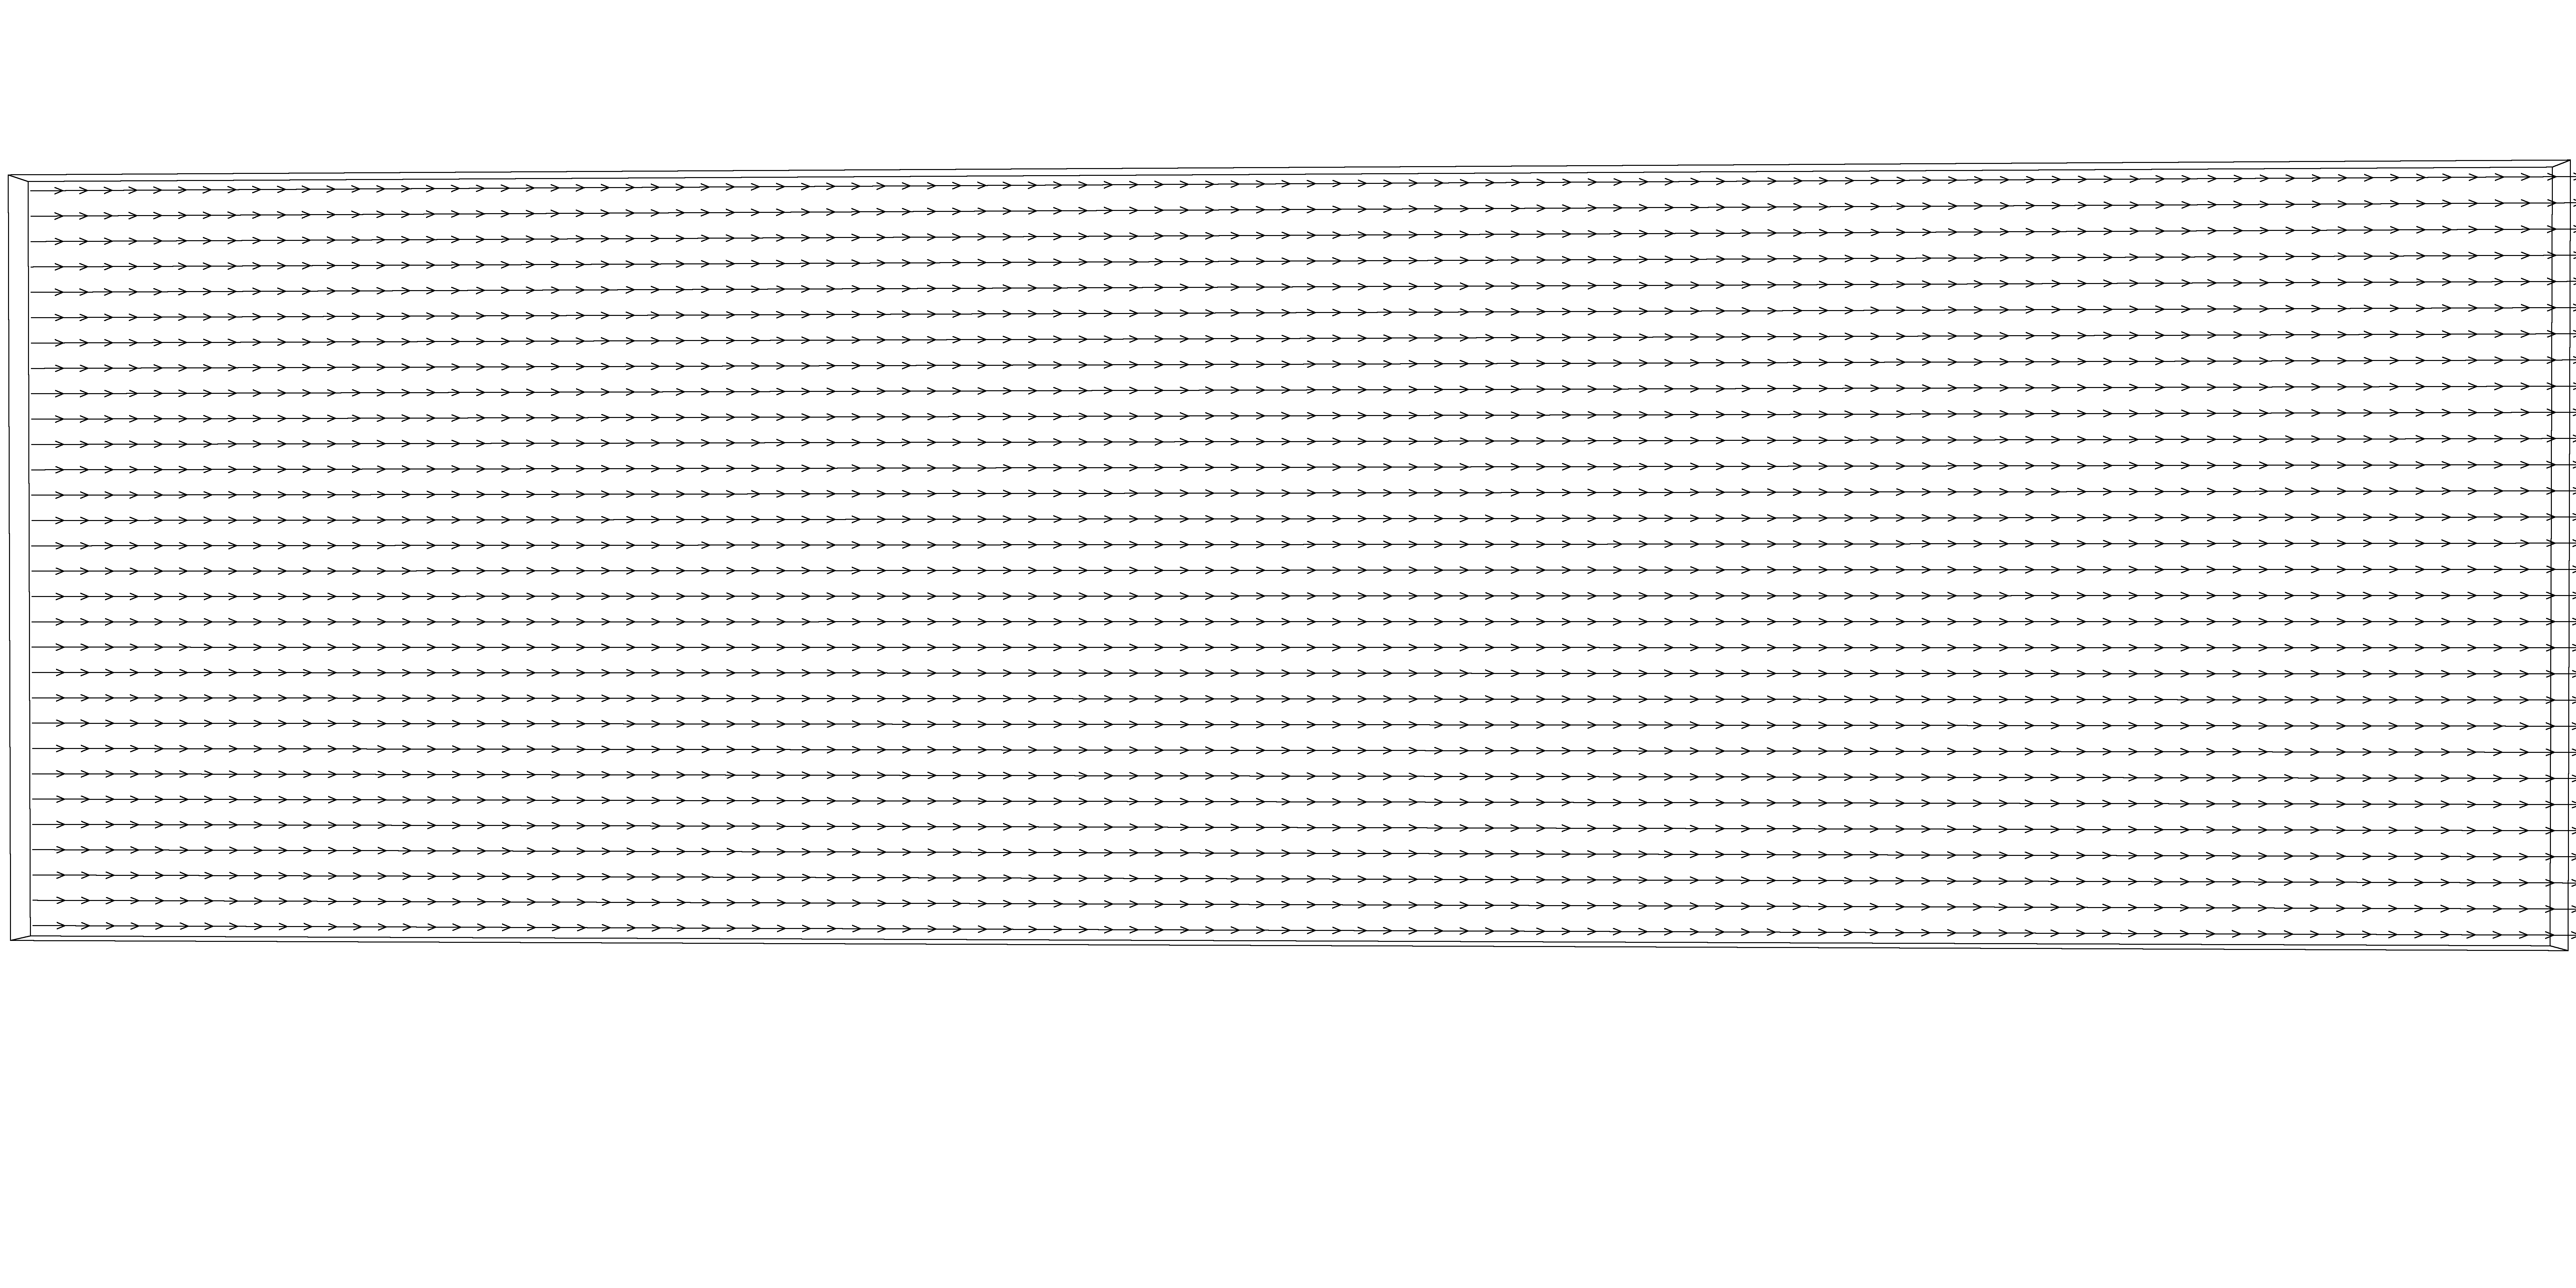
\includegraphics[scale=0.05]{Figures/laminarflow_vectors.png}
\caption{Velocity field of the laminar flow}
\label{LaminarFlowVector}
\end{figure}



\section{Turbulent flow}

Turbulent flow can be considered the opposite of laminar flow. Heavy mixing of fluid particles takes place in a turbulent flow. Important to note is that turbulence is a property of the the fluid flow not of the fluid itself. The motion of the flow itself and
each individual particle can be very noisy and random. In Figure \ref{fig:TurbulentFlowPlain} after a short period of uniform laminar flow the colour streams break up
and become turbulent. There is heavy mixing of colour noticeable and the fluid's path become chaotic. This is due to the viscosity of the fluid itself and also the lenght itself of geometry the fluid
flows along. In general any kind of random variations in a flow's quantities is considered to be turbulent. In Figure \ref{fig:TurbulentFlowVector} this is the velocity: The random fluctuation of the velocity can be seen at a certain moment. the All this factors are represented with the Reynolds number \textbf{Re} which makes it possible to determine if a flow is likely to be laminar or
turbulent. Important ist to understand the difference between fluids and flow since 


\begin{figure}[htp]
\centering
\includegraphics[scale=0.05]{Figures/turbulentflow_plain.jpeg}
\caption{Turbulent flow}
\label{fig:TurbulentFlowPlain}
\end{figure}



\begin{figure}[htp]
\centering
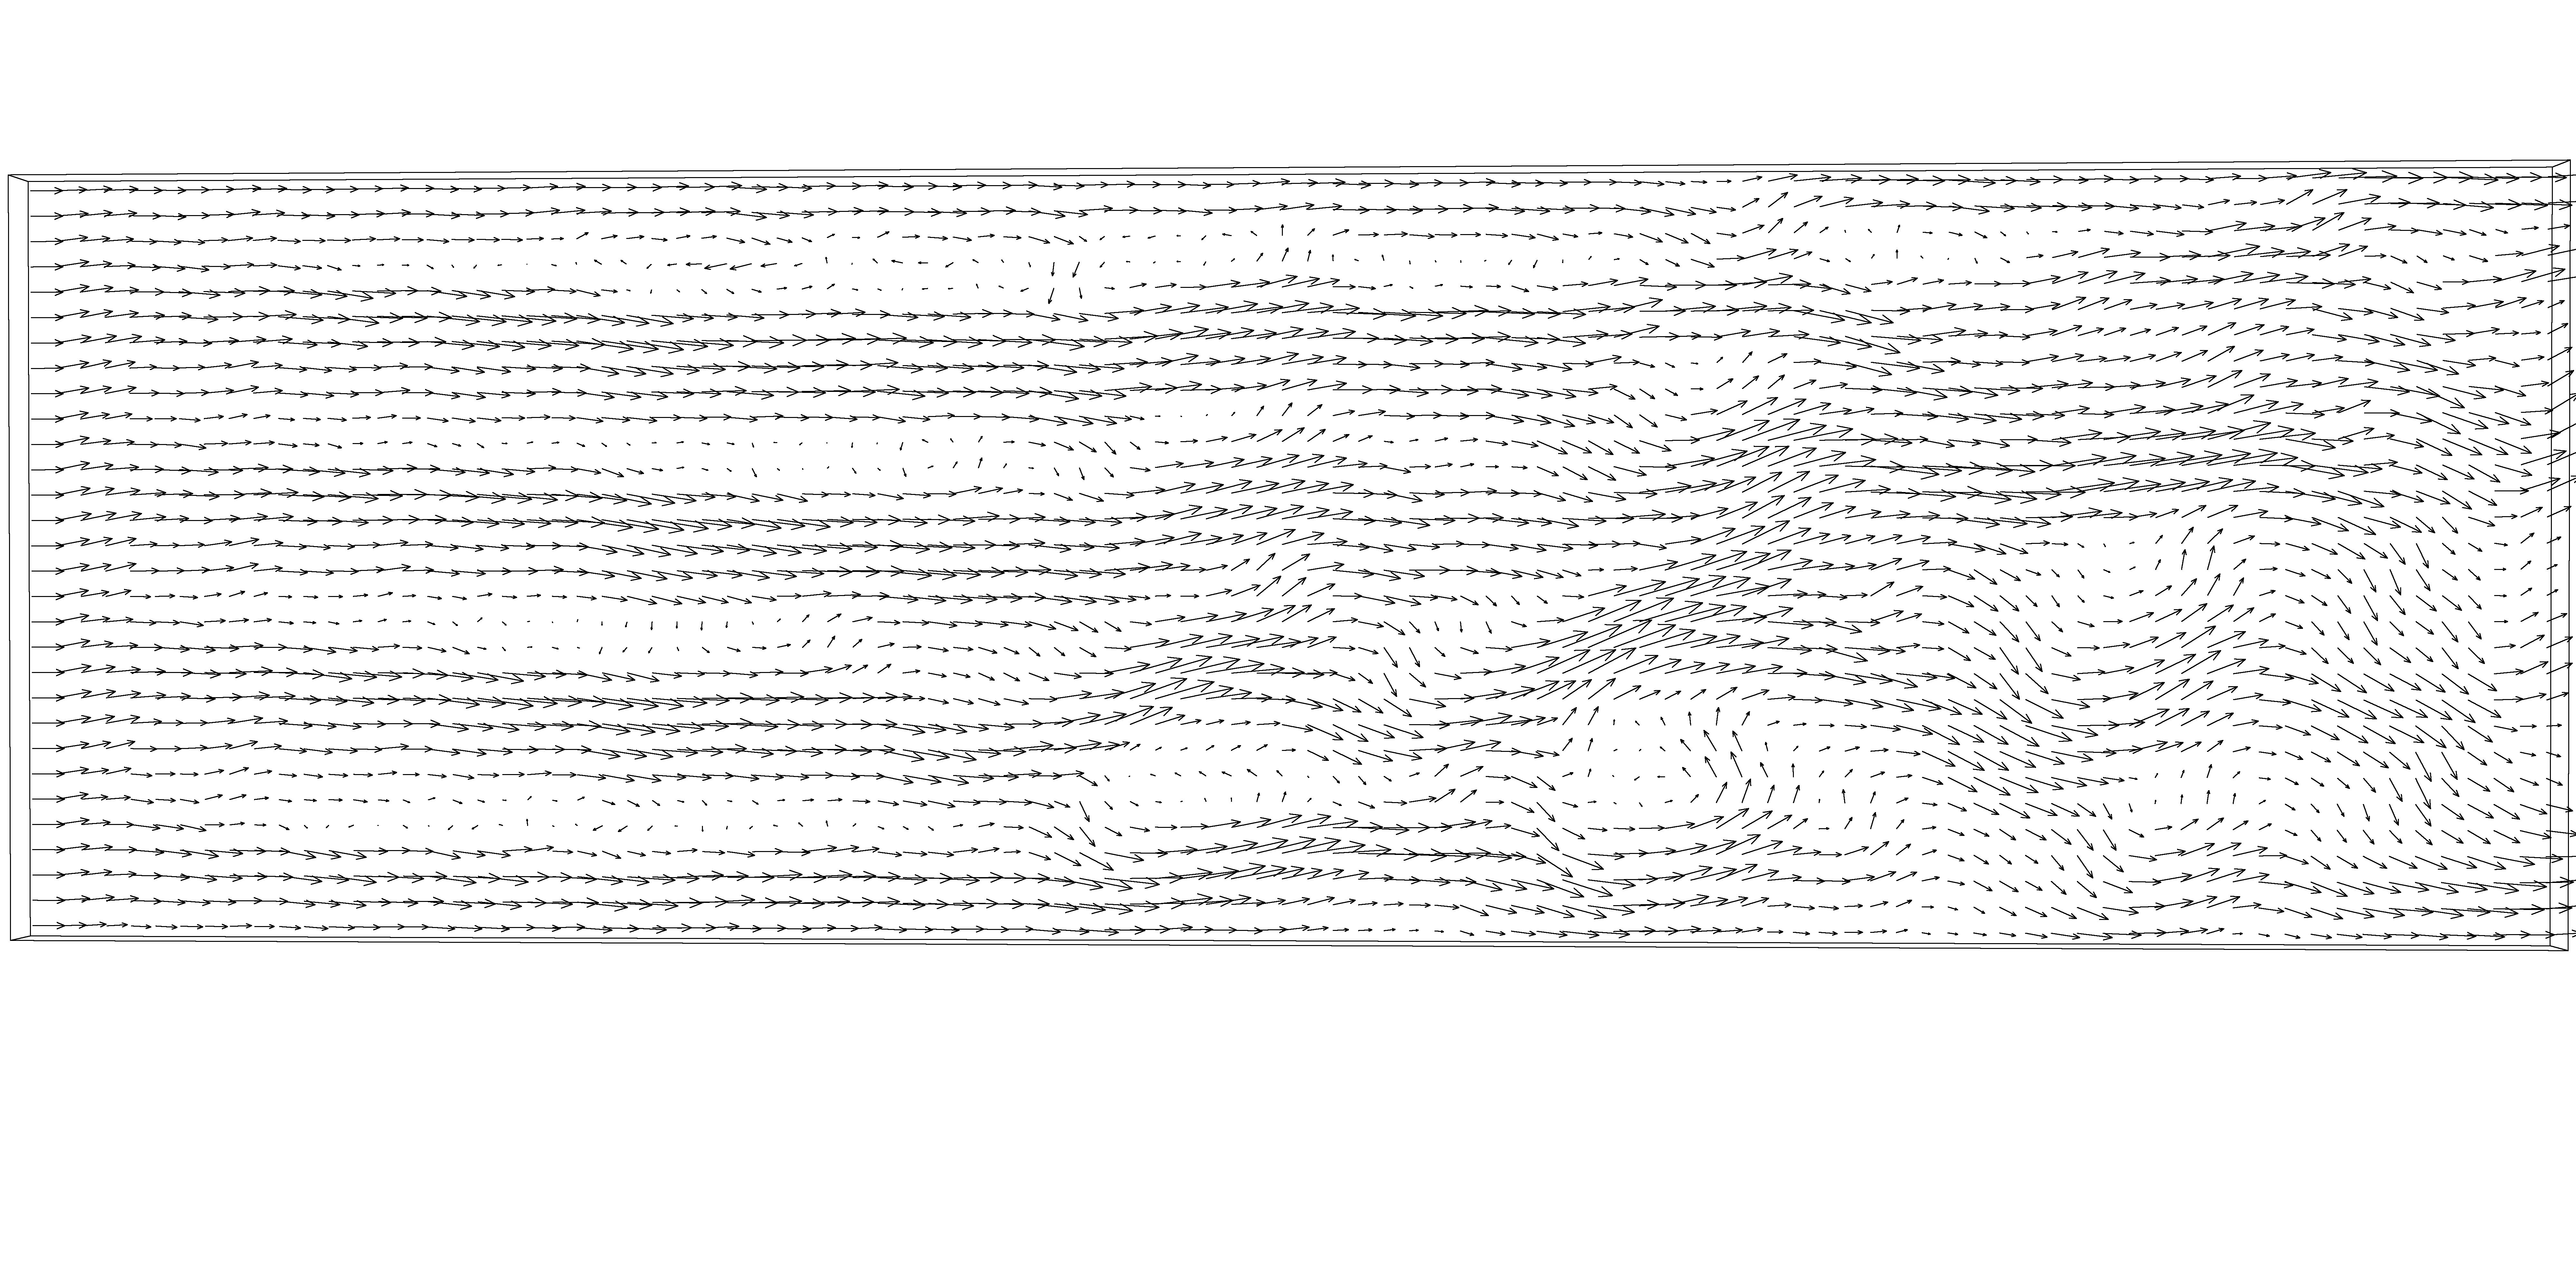
\includegraphics[scale=0.05]{Figures/turbulentflow_vectors.png}
\caption{Velocity field of the turbulent flow}
\label{fig:TurbulentFlowVector}
\end{figure}

\subsection{Reynolds number}

The dimensionless Reynolds number is used to relate inertial forces to viscous forces in a fluid flow. It can be determined as follows and its value helps to estimate if a flow is more likely to be laminar or turbulent. 


\[
Re = 
\frac {VL}{\nu} 
\]


With V denoting the average velocity of the fluid inside or outside the geometry, L
as the characteristic linear dimension or length of the fluid flow (e.g. travelled distance of a fluid) and \(\nu\) as the kinematic viscosity of the fluid.

The linear dimension L varies greatly between different geometry types and is subject to engineering convention. For instance not the lenght but the diameter of a pipe is used when computing Reynolds numbers for the internal flow in respective geometry today. Therfore when comparing Reynolds number as follows one always needs to consider the geometry for which it was computed and can not easily compare Reynolds numbers of different geometry classes.

Laminar flow occurs in general when the viscous forces are dominant, hence the Reynolds number needs to be low. Turbulent flows occur when the inertial forces are dominant. As rule of thumb if the Reynolds number is relatively large the flow is likely to be turbulent (Re > 4000), accordingly small numbers are likely to imply a laminar flow (Re < 2100).
The term "relative" means that the seperation betweeen large and small Reynolds numbers is dependend on the \emph{critical} Reynolds number. This critical Reynolds number determines the thresholds and is geometry dependend.
In 

\begin {table}[htp]
\begin{tabular}{lll}

\end{tabular}
\caption{Table of critical Reynolds numbers}
\end {table}





% Chapter Template

\chapter{Numerical Methods} % Main chapter title

\label{Chapter3} % Change X to a consecutive number; for referencing this chapter elsewhere, use \ref{ChapterX}

\lhead{Chapter 3. \emph{Numerical Methods}} % Change X to a consecutive number; this is for the header on each page - perhaps a shortened title

%----------------------------------------------------------------------------------------
%	SECTION 1
%----------------------------------------------------------------------------------------

\section{Introduction}

In this chapter a overall mathematical introduction to the field of computational fluid dynamics is given. There are several
posibilities to classify and structure the wide field of CFD. In most literature this is done by focusing on the physical properties
of the fluid models itself e.g. \citep{Date2005} resulting in categories like incompressible or compressible fluid dynamics. Since the focus of this
report is not on the physical description of fluids, we will take a different approach and structure the report by the domain discretizations
schemes itself which result in the later Chapters 3 "Mesh-based Methods" and Chapter 4 "Mesh-free Methods". First of all a
brief destinction is made between mesh-based and mesh-free methods. These destinction is followed through the entire chapter
and will conclude in detailed descriptions of both methods given in Chapter 3 and Chapter 4. Afterwards the governing physical Navier-Stokes
equations of CFD are given and explained in detail.
For further reading please refer to \citep{Date2005}, \citep{Cebeci2005}, \citep{Toro2009} and for a comprehensive overview of the mathematical notations in CFD please refer to \citep{Aris1989}.

\section {Numerical simulation proceedings}
Before diving into the physical world of CFD we first take a look at the general approach to solving a physical problem with a numerical simulation. By understanding this process we can lay out the Chapter in a more structured way. Figure \ref{fig:CFDSimProcess} shows this general process for a fluid flow problem and begins with the physical problem in the real world. Before even considering any kind of
computer program or mathematical equation, the physical phenomena that are involved or might appear in the real world have to be understood. Some important examples for this like \emph{turbulent flow} were given in Chapter \ref{Chapter2}. From this point on, one needs to abstract from nature in order to define a computable model. Conscious decisions have to be made whether the apprehended phenomena are relevant enought to
be involved in the mathematical modelling or not. At the beginning of the mathematical modelling process this Chapter will describe in Section \ref{sec:mathperspective} two major and different \textbf{perspectives} in how a observer can perceive a fluid flow. This \textbf{Eulerian} or \textbf{Lagrangian} perspective leads to different mathematical equations which will be discussed later. They have vast implications on the discretization process and simulation speed as it will be shown later.  After that the best approximation to the abstracted flow problem, the physical laws that influence the narrowed down
phenomena need to be indentified and mathematically modeled in the appropriate perspective. Usually this leads to mathematical equations, which are in differential or integral form and describe a continuous behaviour of a physical property. In Section \ref{sec:diff_eq} they are discussed. The most relevant physical laws and equations of fluid flow are given in Section \ref{sec:gov_eq_fluiddy}. In order to be computed by a machine with a finite and discrete number space in
finite time, the \emph{space}, \emph{equations} and even \emph{time} (for unsteady flow) need to be discretized. The discretization process will be explained in Section \ref{sec:Discretization} and in the following Chapters in great detail, since this is the focus of this report. Afterwards the discretized model needs to undergo a in-depth numerical analysis on the amount and type of errors the discretization has caused in comparision to the continuous model. This will be done in more detail in the specific discretization methods in the following Chapters (e.g. \ref{sec:taylor_ser_num_ana}). 
The last following four parts are not the focus of this report and would go beyond the constraints of it. Therefore introduction literature into these topics is given.  
The actual \textbf{Implementation} would take place, leading to a program that would take care of numerical \textbf{Solving} the equations and returning the relevant physical quantities dependent on space and time - the \textbf{Simulation}. These results need to be visualized and in many steps analyzed \citep{Oberkampf2010}.

Furthermore a comprehensive list of commercial CFD simulation programs is given in \citep[pg.139]{Martin2011}. To better understand the efficient solving of large sparse matrices please refer to \citep{Saad2003}.


\usetikzlibrary{calc,trees,positioning,arrows,chains,shapes.geometric,%
    decorations.pathreplacing,decorations.pathmorphing,shapes,%
    matrix,shapes.symbols}

\tikzset{
>=stealth',
  punktchain/.style={
    rectangle, 
    rounded corners, 
    % fill=black!10,
    draw=black, very thick,
    text width=10em, 
    minimum height=3em, 
    text centered, 
    on chain},
  line/.style={draw, thick, <-},
  element/.style={
    tape,
    top color=white,
    bottom color=blue!50!black!60!,
    minimum width=8em,
    draw=blue!40!black!90, very thick,
    text width=10em, 
    minimum height=3.5em, 
    text centered, 
    on chain},
  every join/.style={->, thick,shorten >=1pt},
  decoration={brace},
  tuborg/.style={decorate},
  tubnode/.style={midway, right=2pt},
}

\begin{figure}[htp]
\centering
\begin{tikzpicture}
  [node distance=.8cm,
  start chain=going below,]
     \node[punktchain, join] (intro) {Fluid flow problem};
     \node[punktchain, join] (intro2) {Abstraction};
     \node[punktchain, join] (intro2) {Approximation};
     \node[punktchain, join] (probf) {Mathematical model};
     \node[punktchain, join] (investeringer){Continuous description};
     \node[punktchain, join, ] (perfekt) {Discretization};
     \node (asym) [punktchain ]  {Mesbased or Meshless Methods};
      \begin{scope}[start branch=venstre,
        %We need to redefine the join-style to have the -> turn out right
        every join/.style={->, thick, shorten <=1pt}, ]
        \node[punktchain, on chain=going left, join=by {<-}]
            (risiko) {Space Discretization};
      \end{scope}
      \begin{scope}[start branch=hoejre,]
      \node (finans) [punktchain, on chain=going right] {Model equations Discretization};
    \end{scope}
  \node[punktchain, join,] (disk) {Numerical analysis};
  \node[punktchain, join,] (makro) {Numerical solving};
  \node[punktchain, join] (konk) {Visualization and result analysis};
  % Now that we have finished the main figure let us add some "after-drawings"
  %% First, let us connect (finans) with (disk). We want it to have
  %% square corners.
  \draw[|-,-|,->, thick,] (finans.south) |-+(0,-1em)-| (disk.north);
  % Now, let us add some braches. 
  %% No. 1
  \draw[tuborg] let
    \p1=(risiko.west), \p2=(finans.east) in
    ($(\x1,\y1+2.5em)$) -- ($(\x2,\y2+2.5em)$) node[above, midway]  {};
  \end{tikzpicture}
 
\caption{A CFD simulation process}
\label{fig:CFDSimProcess}
\end{figure}


\section{Eulerian and Lagrangian perspective} 
\label{sec:mathperspective}

While formulating the governing equations of a physical problem like fluid dynamics, there are two fundamentally different perspectives that can be taken by a observer to describe
the behaviour of that physical world. This perspective is also called \emph{observational frame of reference}. The Eulerian perspective depends on a static frame of reference. The Lagrangian perspective depends on a floating frame of reference. From these two perspectives different descriptions of the same problem will result . These have wide implications on the later solving of the formulated equations. They are essential to understand the differences within the Meshbased methods and moreover between them and the Meshfree methods.    In this report the term \emph{frame of reference} is not equivalent with the \emph{coordinate system} of a description. Also to shorten up the Eulerian description is often called simply \emph{Eulerian} and accordingly the Lagrangian description is called \emph{Lagrangian}.

To better understand both perspectives, please consider Figure \ref{fig:Olive_bottle_plain}. It illustrates
a glass bottle of olive oil (grey), which is mixed with spice particles like pepper (black) \footnote{Illustration inspired by Luis Cafarelli's lecture on the NSE. Video link to lecture active on 11th of March: http://vimeo.com/18185364}. The oil is incompressible and the particles are capable of moving freely around in the glass bottle. The observer is able to look inside the transparent glass bottle and identify single particles. These particles can also be seen as abstraction's of fluid parcel therefore both terms are used in exchange in this Section. The entire bottle is shaken, to give the particles and the entire fluid some initial movement. From time $t_{0}$ on the bottle's content is observed, while resting on a table.

\begin{figure}[htb]
\centering
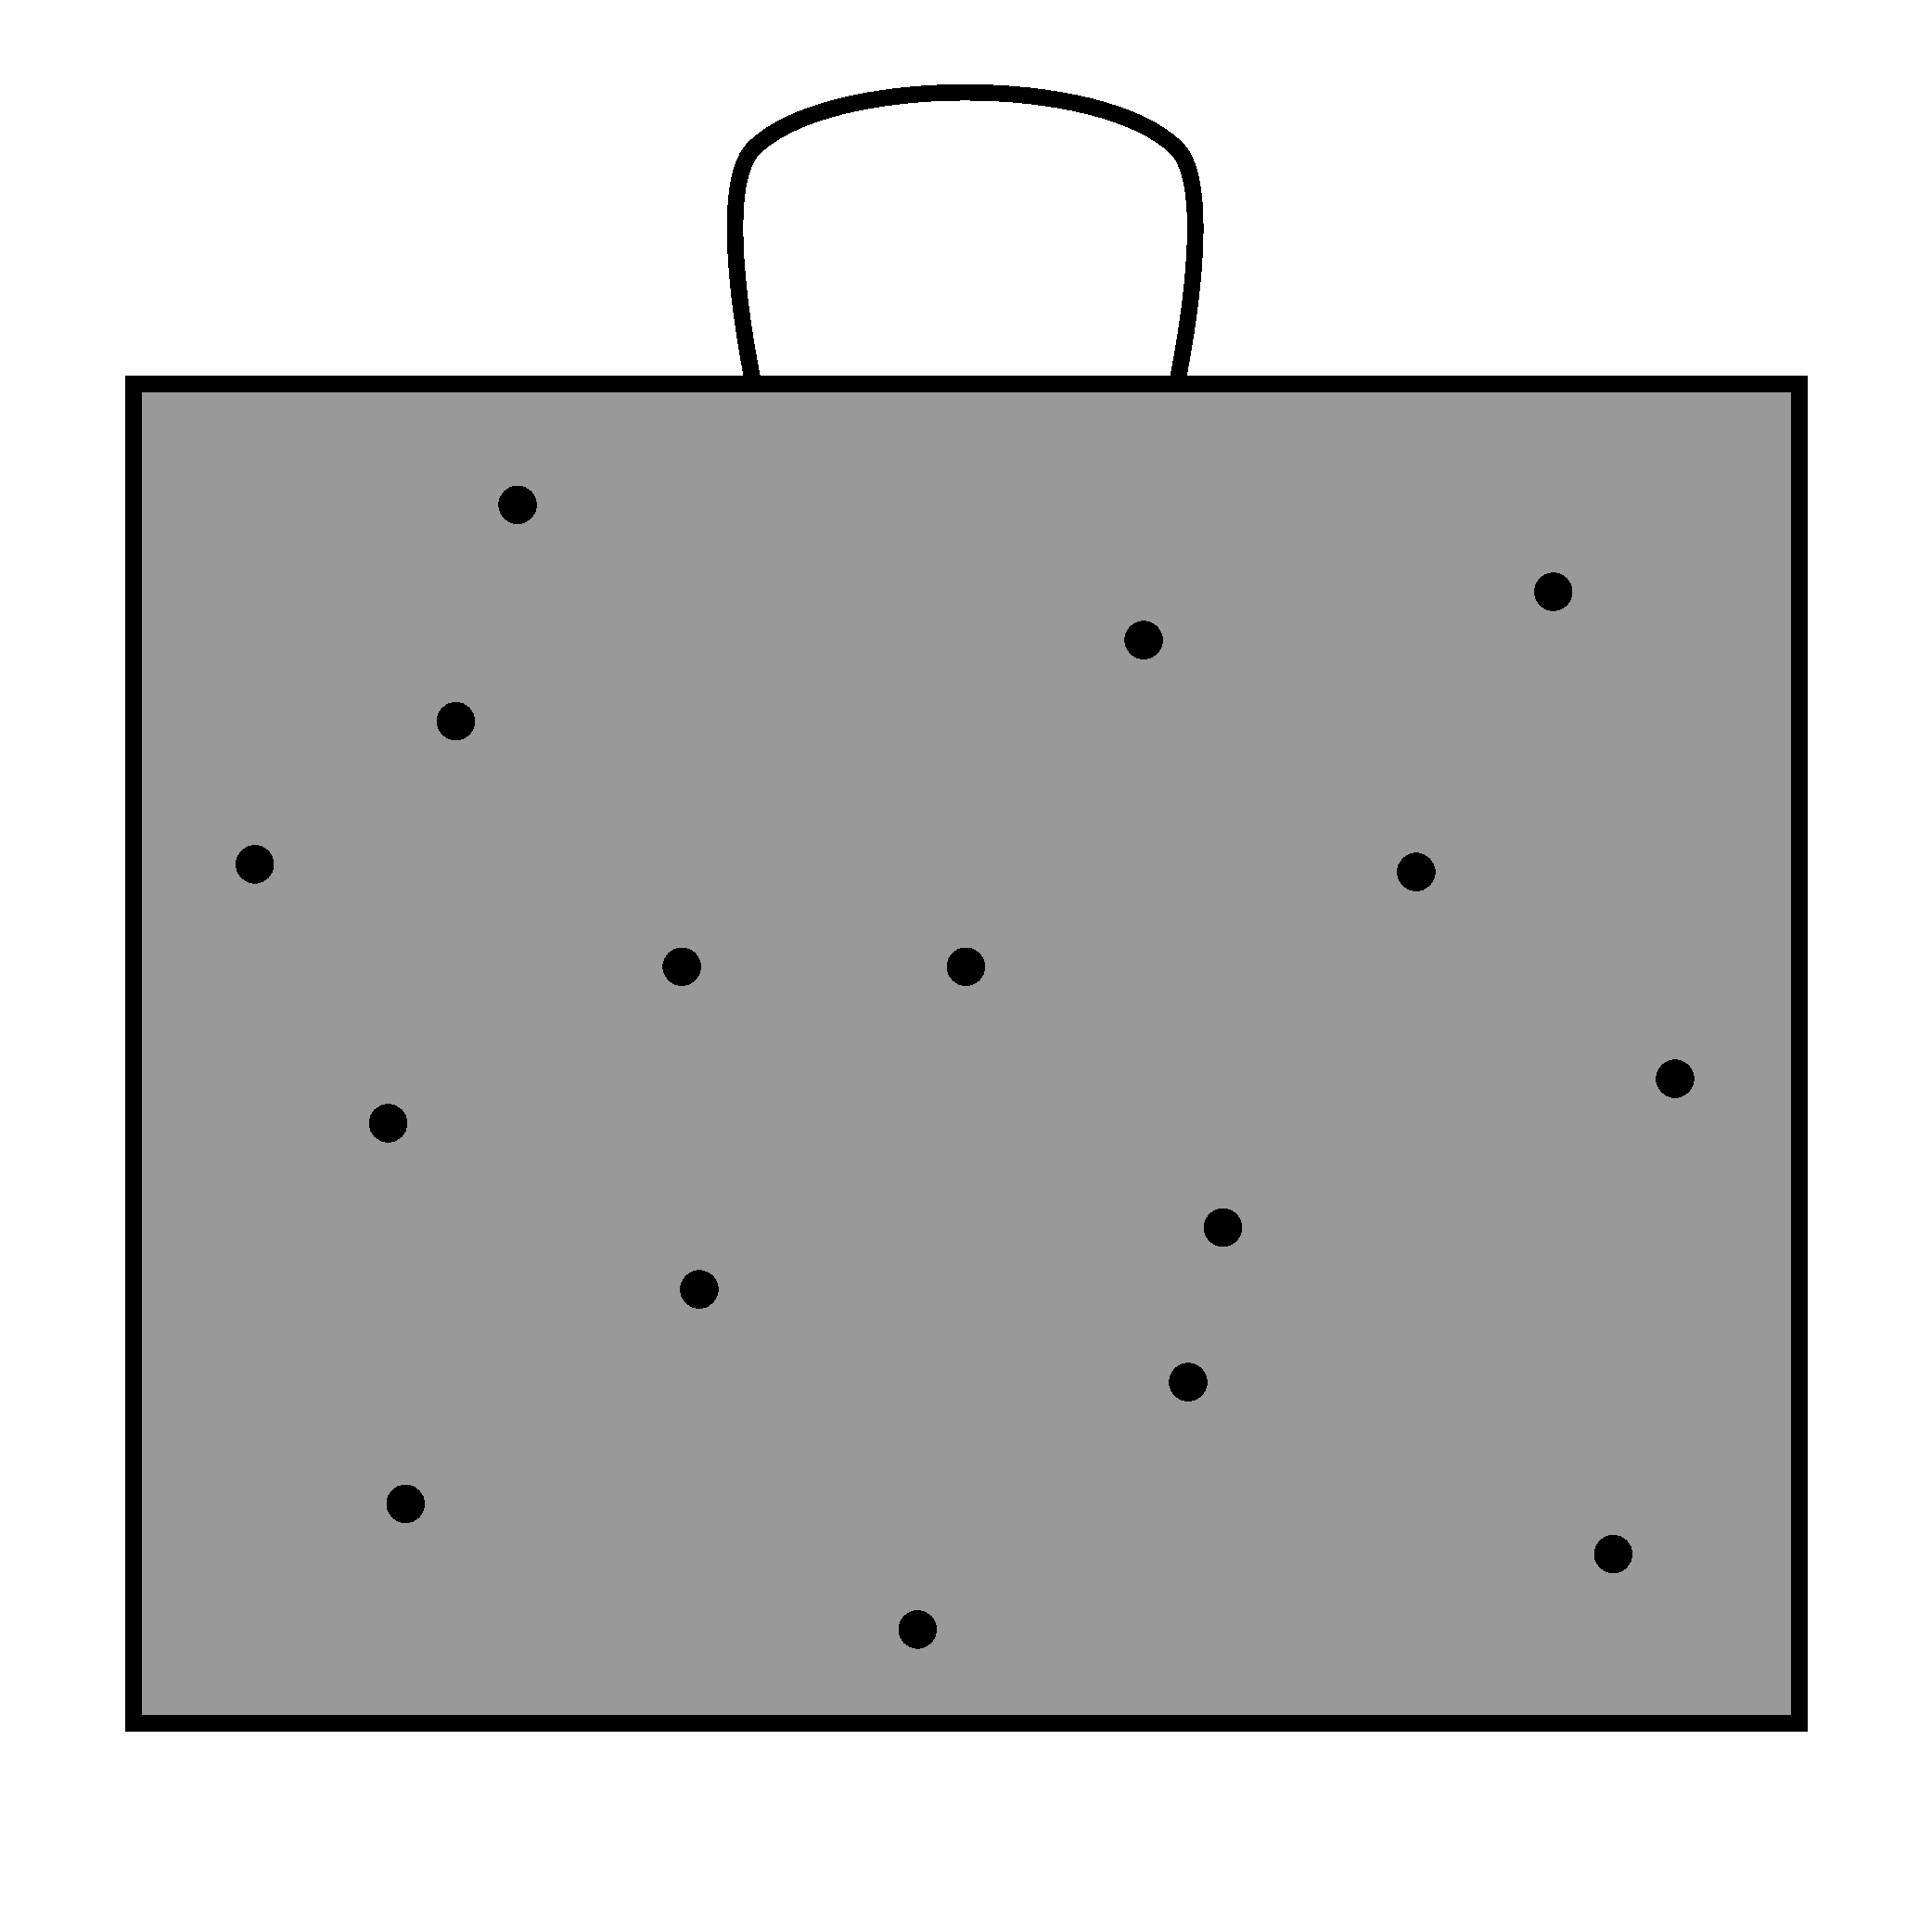
\includegraphics[width=0.4\textwidth]{Figures/olive_oil_can_01.pdf}
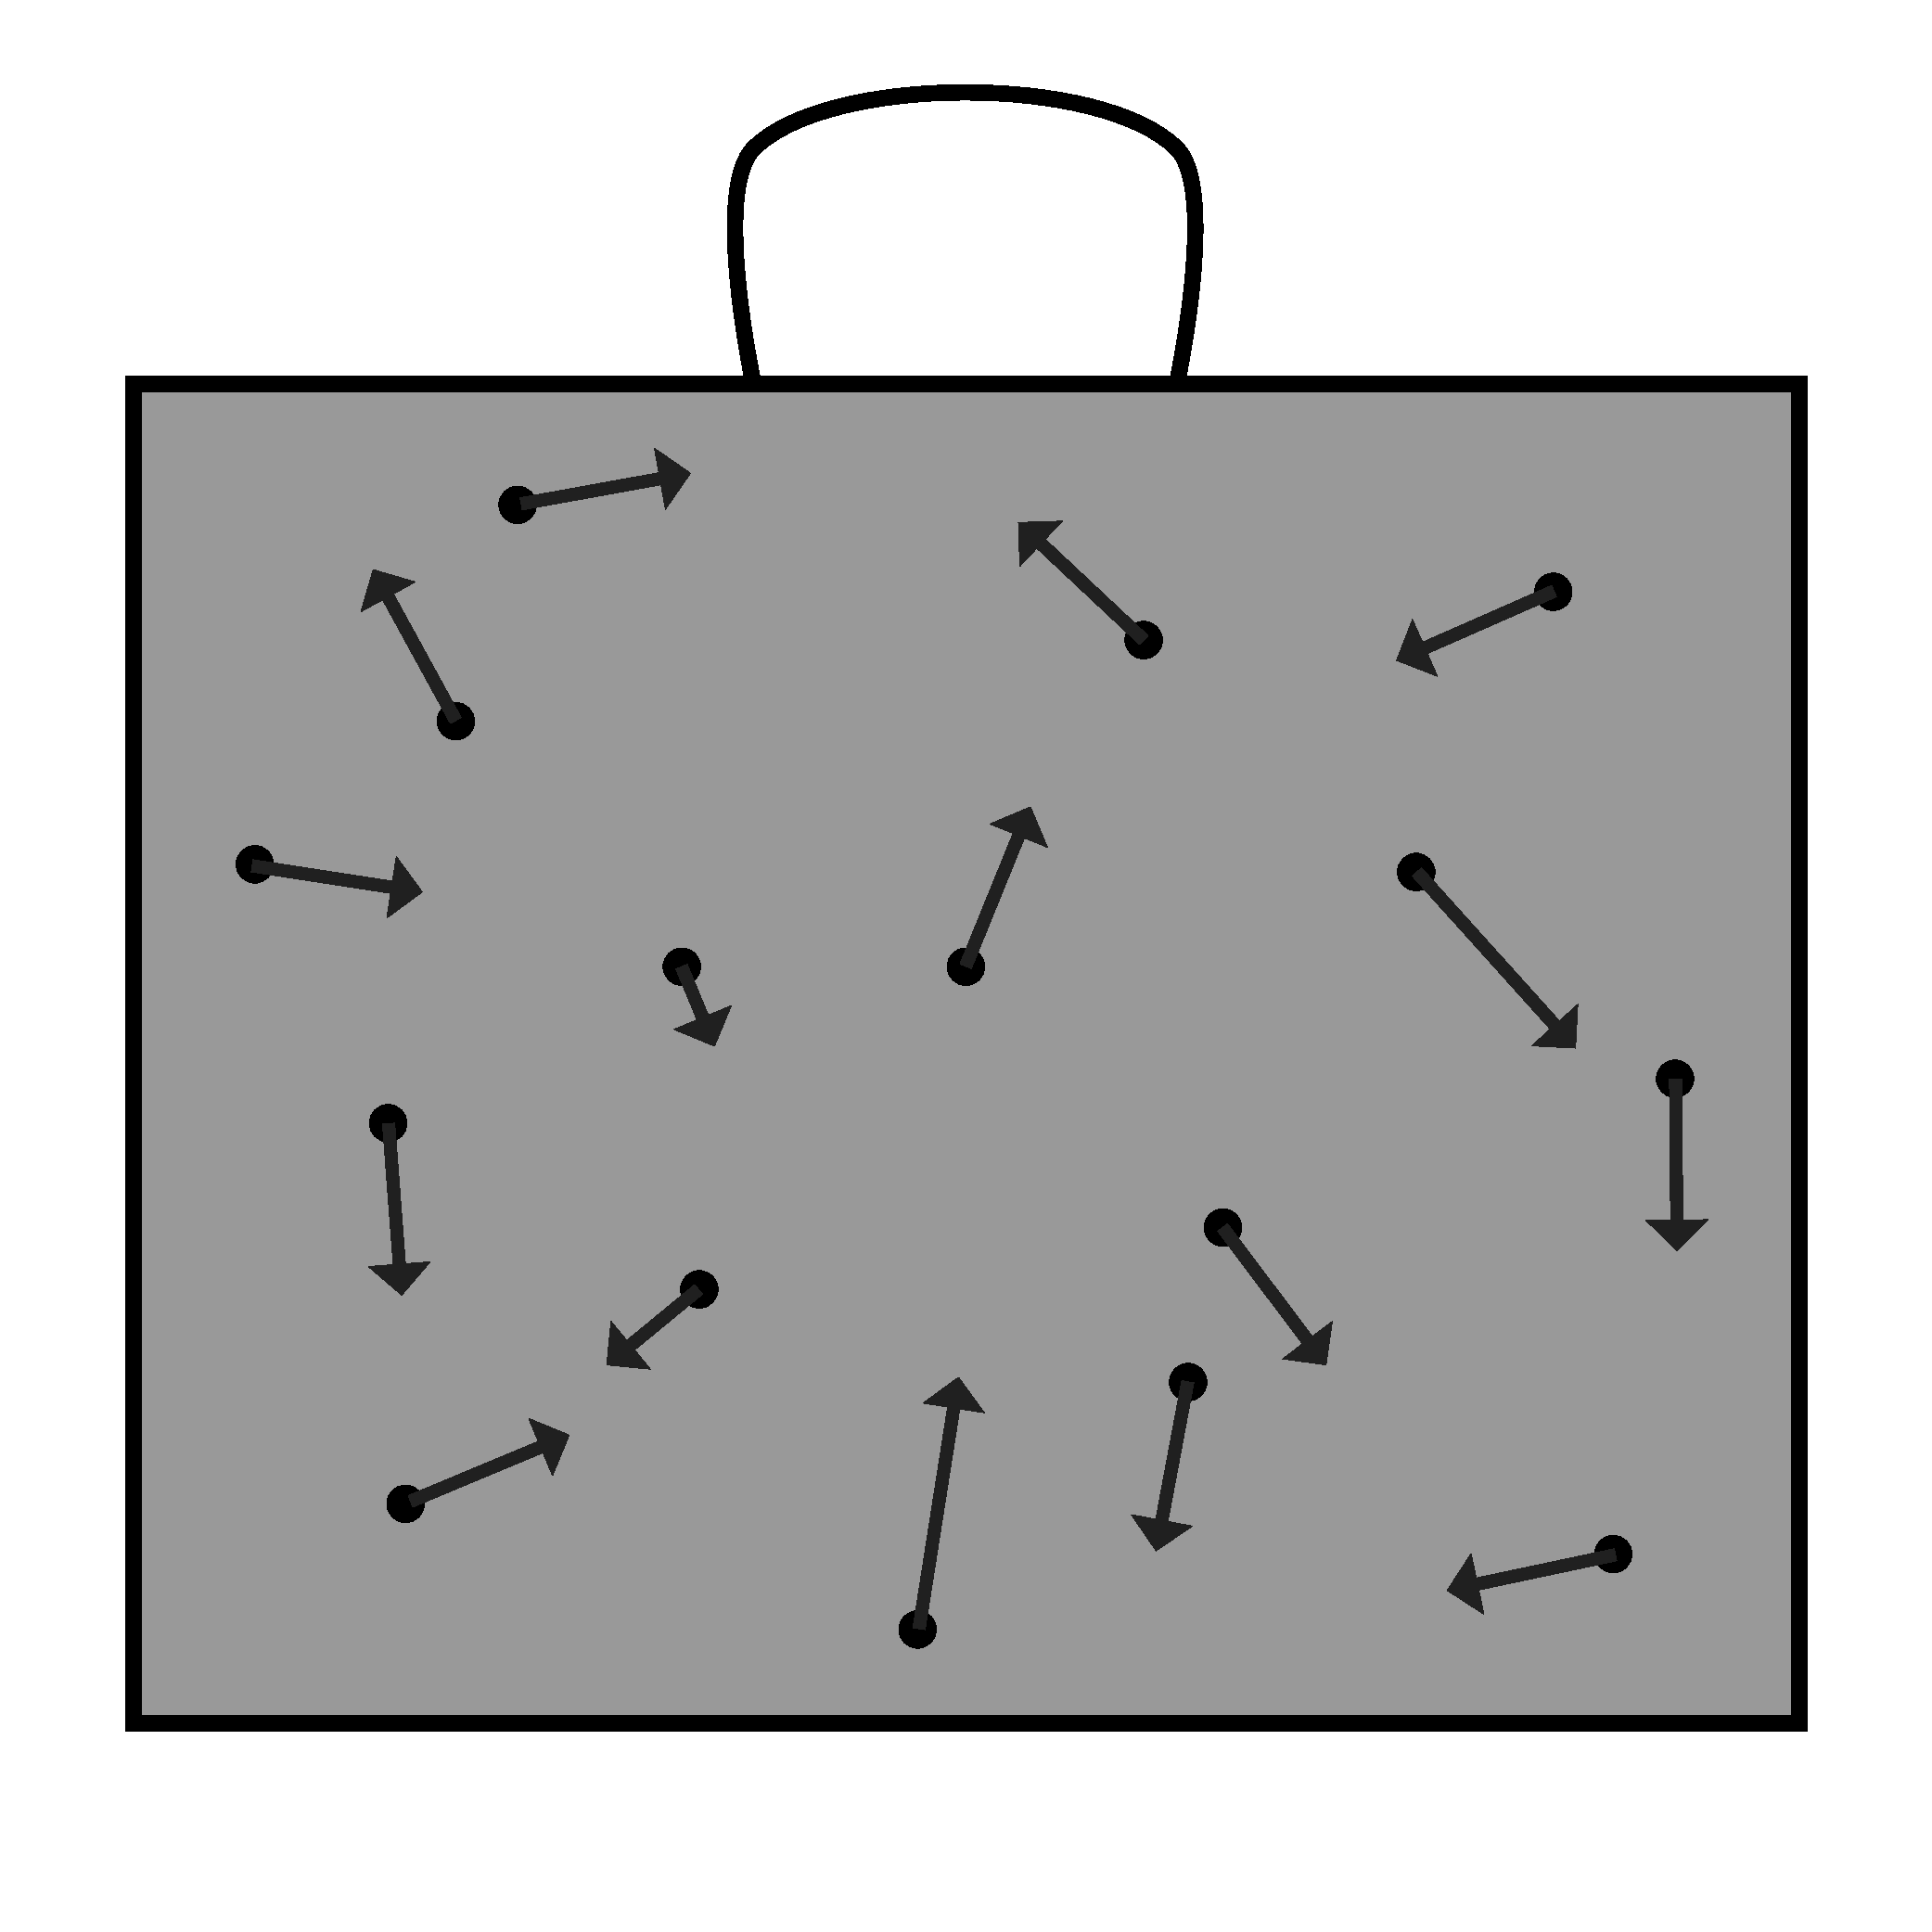
\includegraphics[width=0.4\textwidth]{Figures/olive_oil_can_lagran.pdf}
\caption{Illustration of a glass bottle with Olive oil and spice particles}
\label{fig:Olive_bottle_plain}
\end{figure}

\subsection{Lagrangian Description}
\label{sec:lagrangian_descr}
In the Lagrangian perspective the observer focuses on each separate particle or fluid parcel as it moves inside the glass bottle over time. Therefore the Lagrangian is a \emph{material} description. Each particle is \emph{labelled} $p_{i}$ with $i \in \mathbb{N}_{0}$ at the time $t_{0}$ (resting bottle). The observer moves with each parcel and measures the physical values like velocity (arrow) or mass of it. These values are recorded for each particle $p_{i}$. One can consider these particles to be small moving \emph{sensors} that record physical properties of themselves. 

When the recorded information is presented of a property like speed, this might schematically look like the LHS of Figure \ref{fig:lagr_traj}. Each individual particle has the information of speed at a given time. For the observer this already implies that it is possible to know the fate of each particle and its values for the entire observed time. Furthermore one is able to plot the transport pathways, called \emph{pathlines}, of each individual particle in a transport process as depicted on the LHS of Figure \ref{fig:lagr_traj}.

\begin{figure}[htb]
\centering
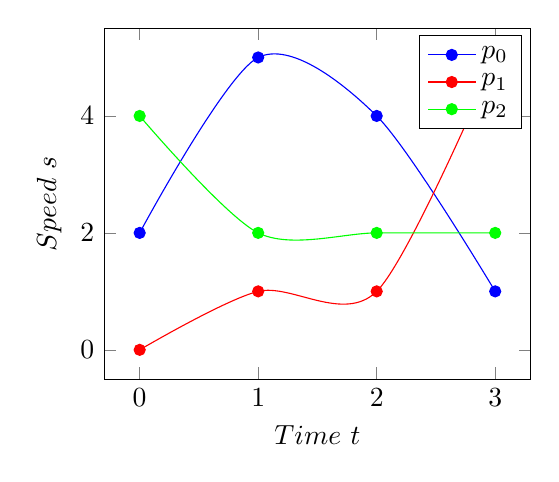
\begin{tikzpicture}
    \begin{axis}[
        xlabel=$Time \ t$,
        ylabel=$Speed \ s$]
    \addplot[smooth,mark=*,blue] plot coordinates 
    {
        (0,2)
        (1,5)
        (2,4)
        (3,1)
    };
    \addlegendentry{$p_{0}$}

    \addplot[smooth,mark=*,red]
        plot coordinates 
        {
            (0,0)
            (1,1)
            (2,1)
            (3,5)
        };
    \addlegendentry{$p_{1}$}

    \addplot[smooth,mark=*,green] plot coordinates 
    {
        (0,4)
        (1,2)
        (2,2)
        (3,2)
    };
    \addlegendentry{$p_{2}$}    
    \end{axis}
    \end{tikzpicture}
    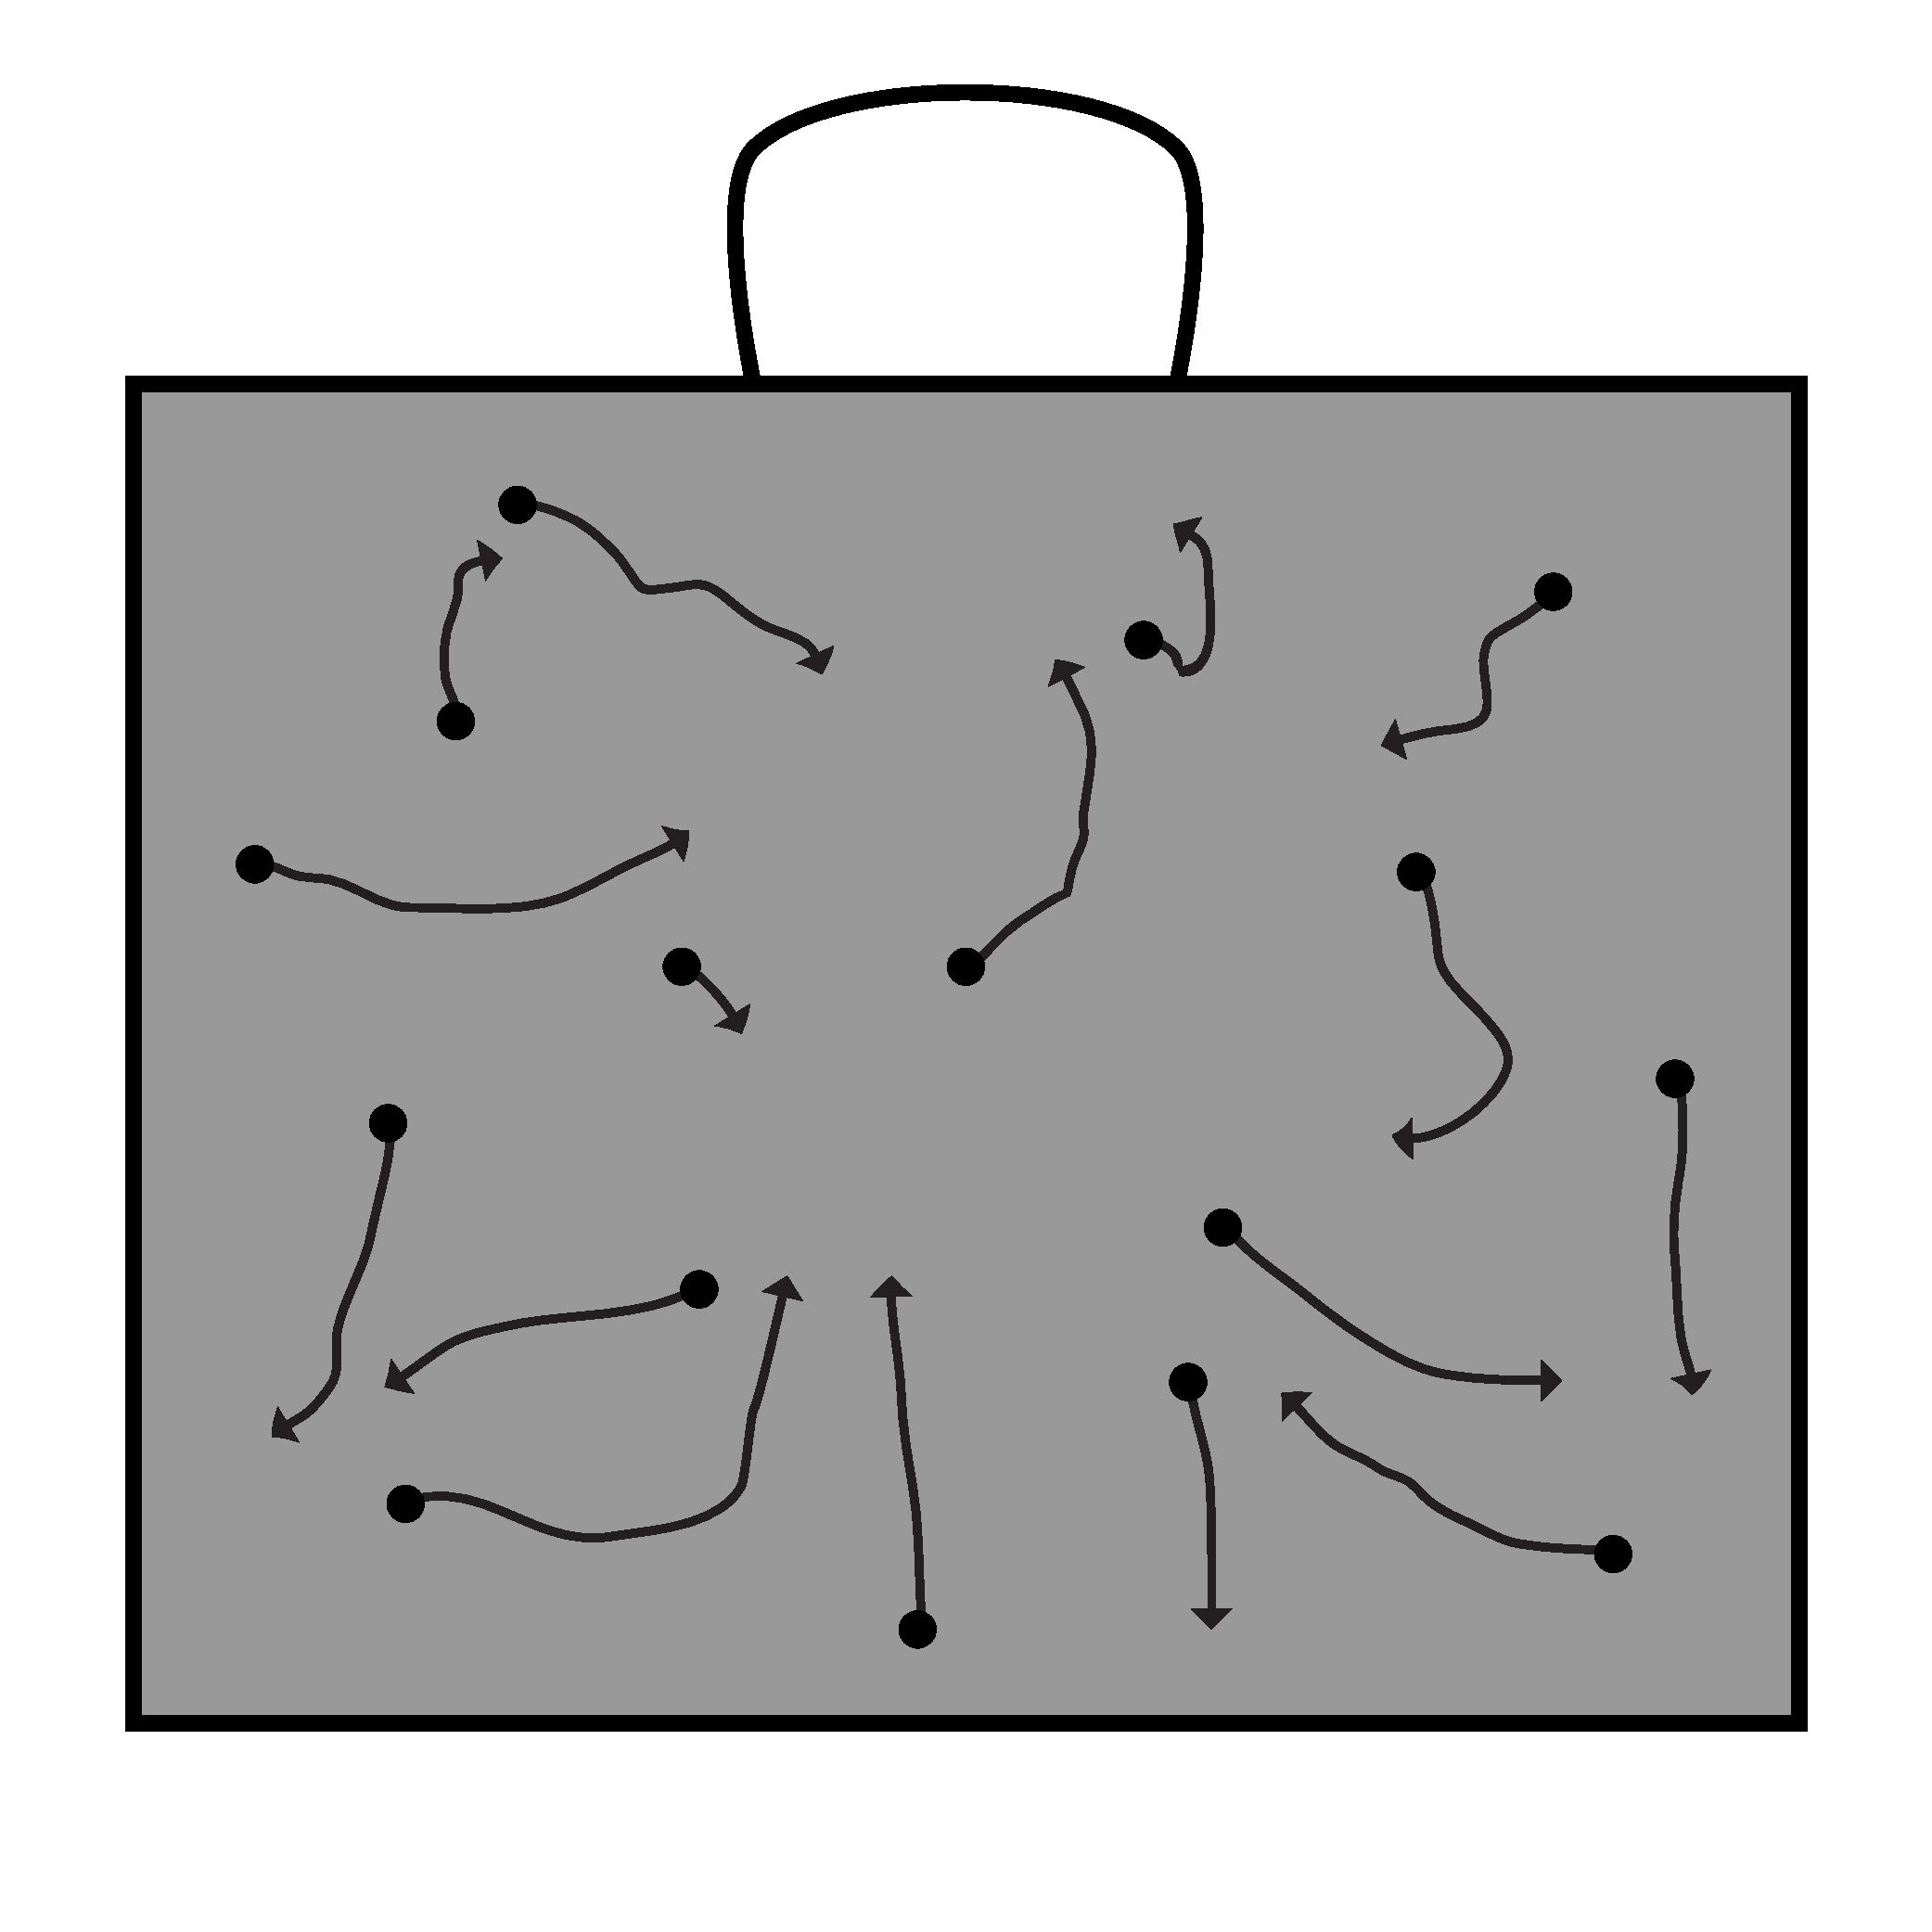
\includegraphics[width=0.4\textwidth]{Figures/olive_oil_can_lagran_pathlines.pdf}
    

\caption{Schematic diagram of particle's speed and pathlines in Lagrangian perspective}
\label{fig:lagr_traj}
\end{figure}




\subsection{Eulerian Description}
\label{sec:eulerian_descr}

In the Eulerian description the observer does not follow individual fluid parcels. He rather rests and focuses on certain selected locations in the domain of the glass bottle. Therefore the Eulerian is a \emph{spatial} description. To better identify these observation locations, a rectangular mesh is drawn onto the bottle with the intersections being the points of interest. In Figure \ref{fig:eulerian_bottle_observer} this is illustrated with hexagonal observer nodes that are located on the intersection points of a rectangular mesh. This mesh discretizes
the spatial domain of the glass bottle (see \nameref{subsec:eulerian_mesh}). A fluid parcel is only noticed over time and measured by the observer when it passes through a observer node, this is depicted with the red hexagons. So in contrast to the Lagrangian perspective, the \emph{sensors} are static in location. Consequently in the Eulerian the observer is not capable of knowing the trajectories of all fluid parcels.

\begin{figure}[htb]
\centering
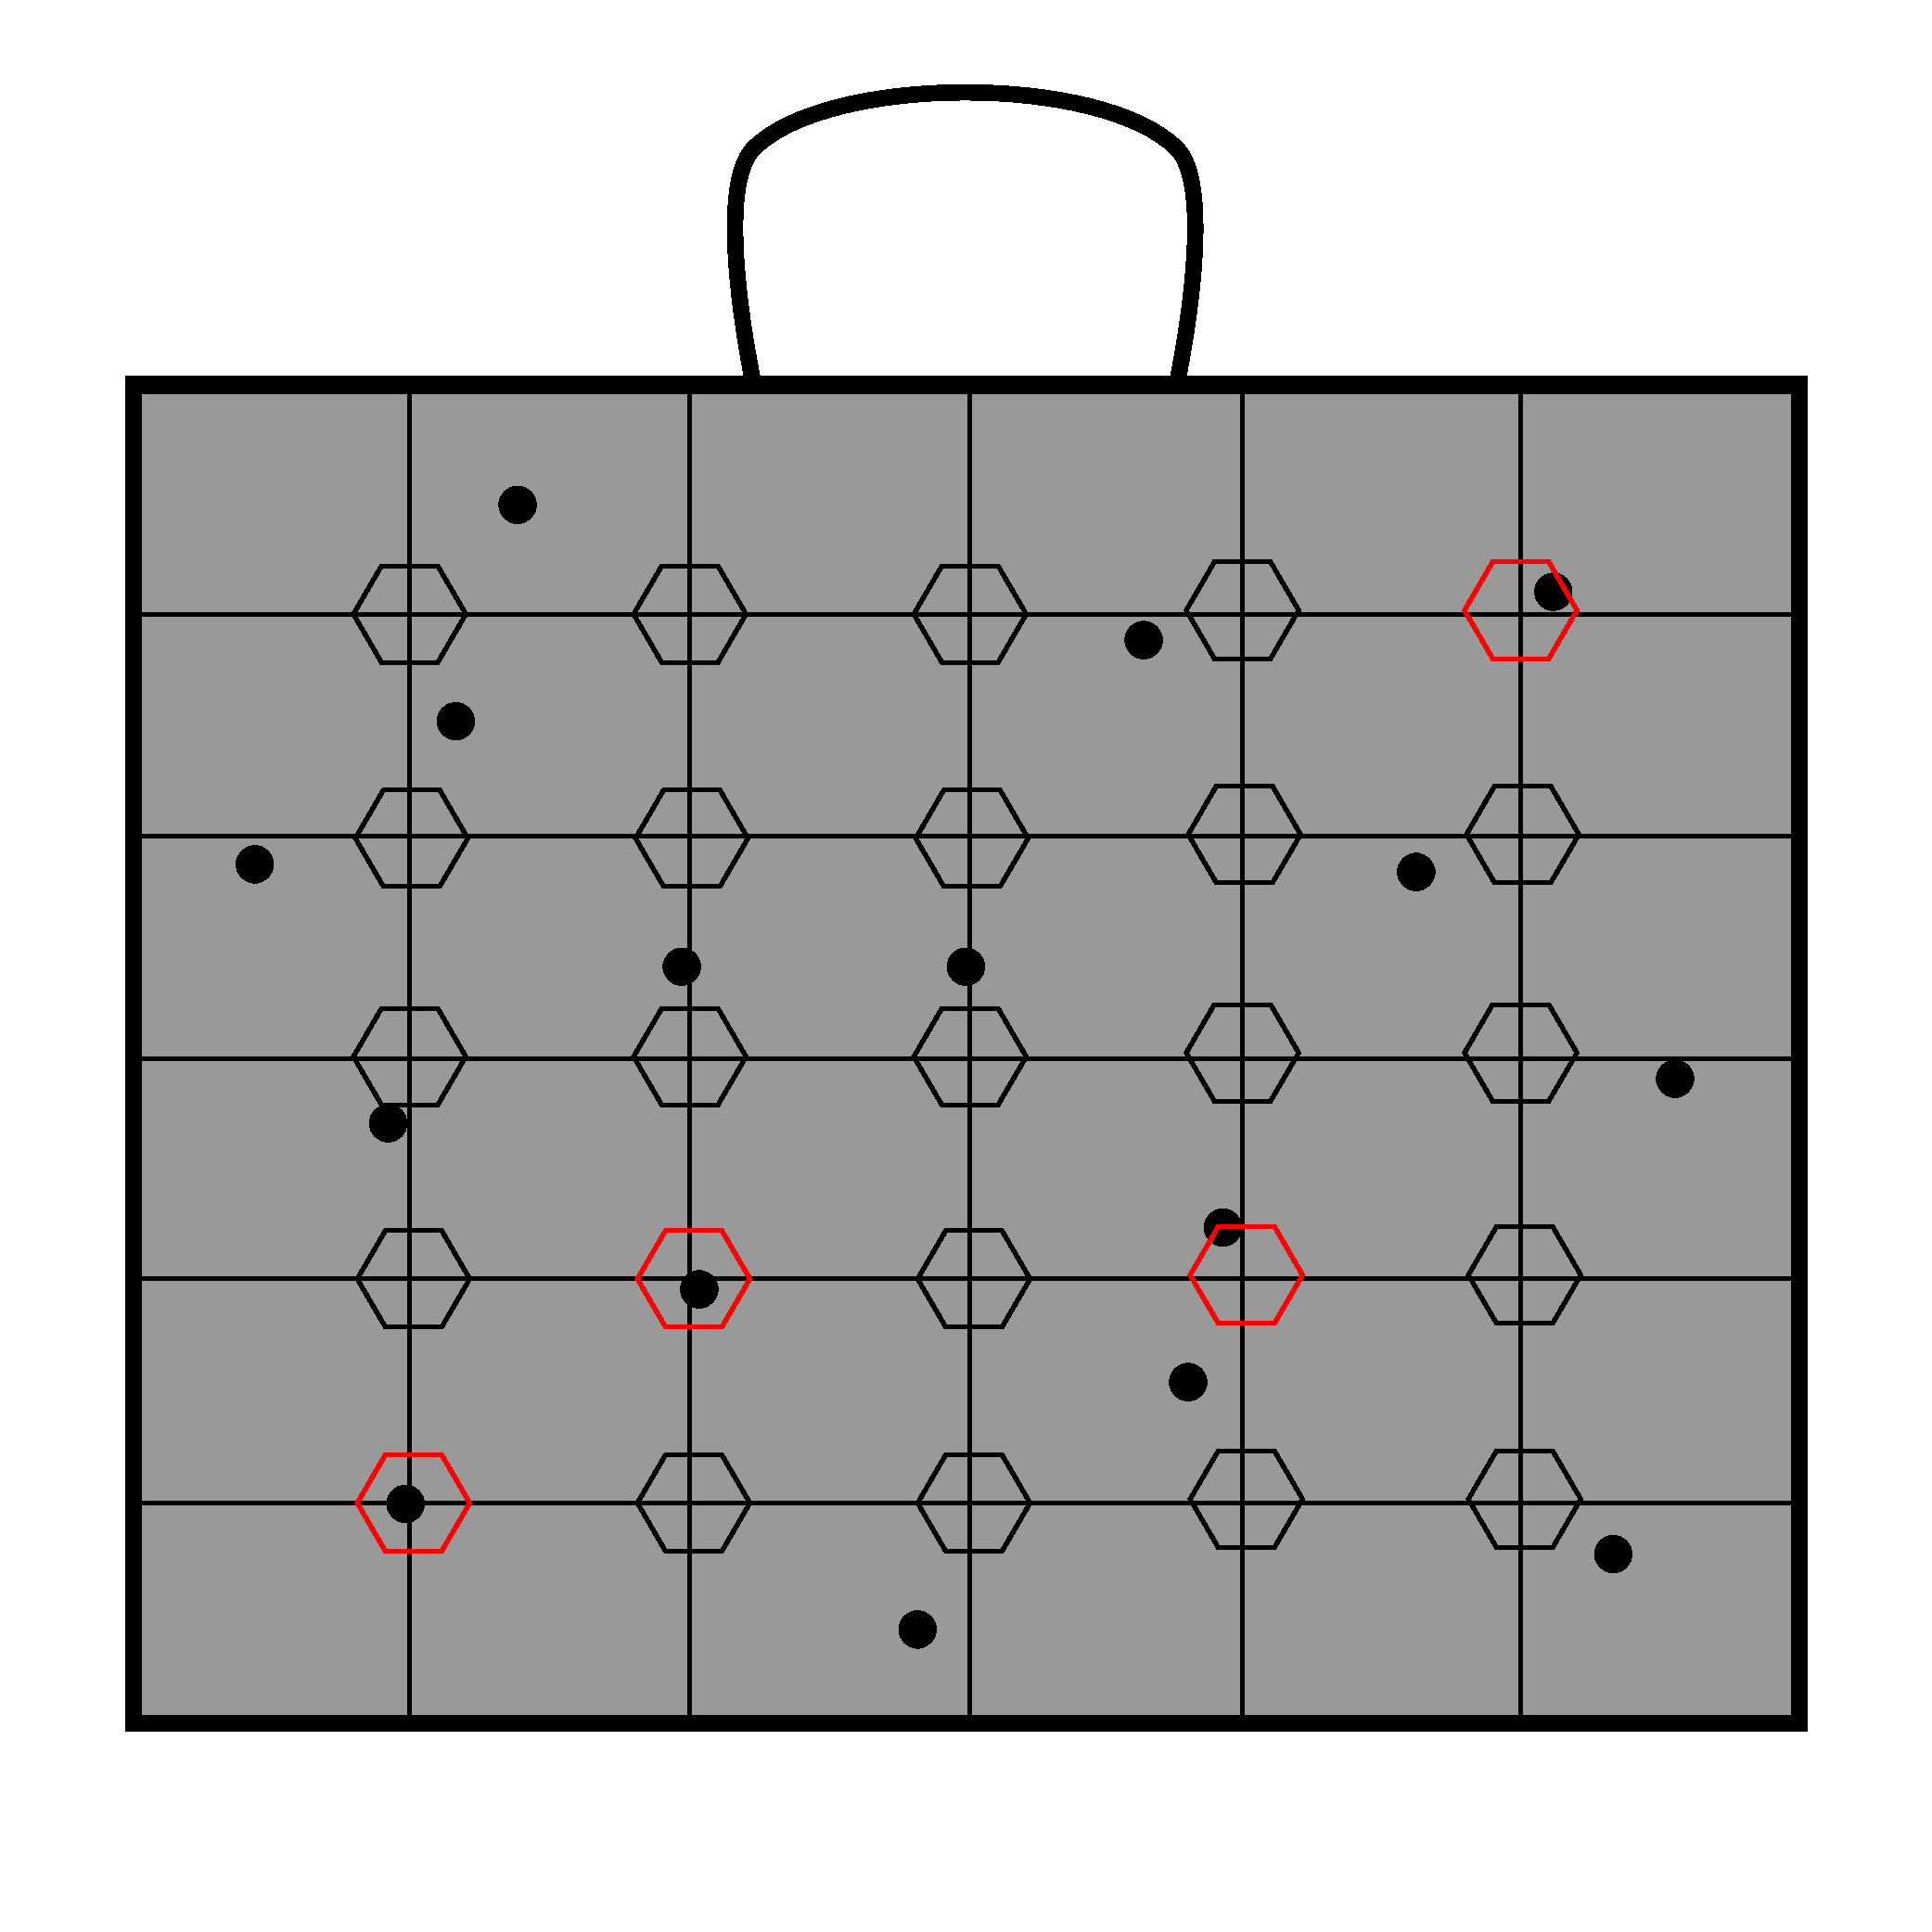
\includegraphics[width=0.4\textwidth]{Figures/olive_oil_can_eulerian.pdf}
\caption{Illustration of hexagonal observer nodes inside a rectangular mesh in Eulerian perspective}
\label{fig:eulerian_bottle_observer}
\end{figure}


\subsection{Lagrangian vs. Eulerian Description}
To bring both descriptions into a mathematical framework we first start with the Lagrangian. As mentioned above each individual particle is labeled $p_{i}$ at time $t_{0}$ when the bottle is released to rest. This label is a vector of the fluid properties or the particles Cartesian coordinates at the time of release. The Lagrangian observer follows the particle after time $t_{0}$ and notes down the position of this individual particle at time t as:

\begin{equation}
X_{i}(p_{j}, t_{0} | t)
\end{equation}

In Eulerian description the position of a observer is simply $x_{i}$. The above situation that this Eulerian observer is able to recognize a fluid parcel (red hexagons) is only given when:

\begin{equation}
x_{i} = X_{i}(p_{j}, t_{0} | t)
\end{equation}

Similar to this the velocity relation in Eulerian and Lagrangian perspective is given by:

\begin{equation}
v(x_{i},t) = \frac{\partial X_{i}}{\partial t} (p_{j}, t_{0} | t)
\end{equation}

Where the LHS denotes the velocity v from the fluid parcel detected by a Eulerian observer, the RHS denotes the Lagrangian version. In similar manner the relation to the rate of change of other physical quantities like heat or momentum can be found. A important mathematical instrument for this is the Stokes derivative, also called material derivative.

\subsection{Implications on Fluid Dynamics}

In Fluid Dynamics the transport or \emph{flux} of fluids is of primary interest. In Eulerian description the flux can only be estimated correctly when there is a dense spatial and temporal coverage of observing nodes.

Flux processes itself are fundamentally a Lagrangian quantity and therefore easier to describe in this perspective. As we will see in the following Chapters, methods with a Eulerian description like FVM have ways to estimate the flux in a certain region. But with more complicated, even deforming, geometry the Lagrangian description is capable of handling these changes far better (e.g FEM). The Lagrangian is used widely in astrophysics, where the gravity of stars, planets and galaxies interact within a vast space of vacuum without any interesting behaviour. The focus lies here on relatively few objects/parcels in comparison to the immense
spatial distribution of those. Concerning CFD a rough estimation can be already made that the Lagrangian is better for (many) single fluid parcels that are of interest and can have great deformation behaviour. As we will see in this report this is not entirely true. A method in Lagrangian description and a attached mesh can lead to more problems with deformations in CFD than a Eulerian method (see \nameref{sec:main_fem}). In addition
leaving out a mesh in a Lagrangian method, as it is done in \nameref{Chapter 5}, brings out the deformation robustness concerning CFD. For further reading please refer to \citep{Bennett2006}.

\section{Differential equations}
\label{sec:diff_eq}
In the following Section the \nameref{sec:gov_eq_fluiddy} are presented. These equations rely heavily on
higher mathematics and describe the fluids properties and flow with various differential equations. This section should brush up very briefly the knowledge on differential equations for the novice reader. Of utmost significance is the classification of partial differential equations into parabolic, hyperbolic and elliptic types, since the later numerical discretization methods are not equally capable of solving all of them efficiently.
\subsection{Ordinary Differential equations}
Ordinary Differential equations (ODE) occur in many CFD terms. Of special interest for this report are they because they are present in the \nameref{Chapter 5} method.

%Runge Kutta 
\subsection{Partial Differential equations}
%PDEs

\subsection{Divergence theorem}
\label{sec:div_theorem}

\section{Implicit Methods}
\section{Explicit Methods}

\section{Boundary Conditions}
\subsection{Von Neumann Conditions}
\subsection{Dirichlet Conditions}

\section{Governing equations of Fluid Dynamics}
\label{sec:gov_eq_fluiddy}

As we have seen in Chapter \ref{Chapter2} there are many different types of flow in Fluid Dynamics and many physical properties that define them. As this report focuses on unsteady flow, a key finding of Science is that the \emph{entire} motion and behaviour of a fluid flow can be indicated by the conservation laws for \textbf{momentum}, \textbf{mass} and \textbf{energy}. We will use the already explained general form of conservation laws and apply them to these three properties leading to the Euler equations and Navier-Stokes equations. These equations are of a very general Nature and need supporting physical laws when they are applied to a more specific fluid type like \nameref{sec:incompress_fluid}. This can lead to a massive simplification of the NSE, since depending on the nature of the specified fluid type many equations become simpler or even zero out. Moreover also external properties like forces need be considered, when they actually influence the fluid itself. An excellent example of such can be found in \citep{Warner2010} where in order to model the behaviour of fluid packets in our atmosphere also the coriolis forces and Earth's gravity influence the fluids momentum. The set of equations are usually coupled to a certain degree, which complicates solving them. 

 

\subsection{Conservation of Momentum}



\subsection{Conservation of Mass}

The conservation of mass is a key property of fluid flow. In a closed fluid system
no mass is created at any point or destroyed. This fact is of great use later on in FVM were withing a subdivided discrete volume no material sources or sinks exists.
The physical changing value of the fluid's density $\rho$ is bound by this law in the overall system. The fluids mass only is transported by convective flux, which considering the above notations of a conservation law leads to:

\begin{equation}\label{eq:con_mass_1}
\frac {\partial}{\partial t} \int\limits_{\Omega} \rho d \Omega +
\oint\limits_{A} \rho \vec{v} \cdot d \vec{A} = 0
\end{equation}



\subsection{Conservation of Energy}





Mathematical model of fluid motion
Form? integral form ...auch sections machen?

\subsection{Euler equations}
The Euler equations don't cover viscosity and any kind of heat conduction effects. They are of hyperbolic nature in space and time. Therefore these equations only cover \nameref{sec:invisicid_flow} of fluids.

\begin{equation}
\rho \frac{dv}{dt} = 
\rho ((\nabla \cdot v)\cdot v + \frac {\delta v}{\delta t }) =
f - \nabla p 
\end{equation}


\subsection{Navier-Stokes equations}
\label{sec:NSE_main}
The Navier-Stokes equations (NSE) are a set of equations to describe (in)compressible
viscous fluid flows. Therefore they can be seen as a extension and a more accurate version of the Euler equations that now include viscosity and heat conduction. Formulated by the French physicist Claude-Louis Navier with contributions from the Irish physicist George Stokes in the 19th century these set of equations are the cornerstones of today's understanding of fluid dynamics. The set of Navier-Stokes equations are in general parabolic equations in time and space. 

%Assumptiuons and preconditions


%Initial conditions
%Boundary conditions
%Numerical Solver to solve the equations

 

%Continuum laws



%In Fluid Mechanics 
%page 116




\section{ The Concept of Discretization } \label{sec:Discretization}

The governing ordinary and partial differential equations that occur in many domains of physics describe
\emph{continuous} models. Solving those equations analytically would result in exact continuous solutions. However in practice
a exact analytical solution is not possible and needs to be replaced by a approximation that is found numerically with the aid of computers.
Modern digital computers are only capable of representing a finite and discrete amount of numbers with a finite amount of computational time, memory and storage.
Therefore any continuous model has to be transferred into a discrete model. This process is called \emph{discretization} and for a general spatial or temporal domain $ \Omega $ this is called \emph{domain discretization}. When this transfer happens several different kinds
of error are introduced into the approximate solution. Among others the most important ones are the \textbf{number representation error}, \textbf{roundoff error} and \textbf{truncation error}. For further reading on these error types please refer to \citep[pg.8]{Press2007}.

This section continues the numerical discussion of the CFD equations by focusing on the discretization process. The \emph{continuous} Navier-Stokes equations need to be 
discretized in order to solve them. Since this report focuses on unsteady fluids, the given equations are time-dependend. The differential equation in CFD always have a spatial component and in our case also have time dependent components in them. In the process of discretization these dimensions have to be discretized. This results in approaches for \textbf{spatial} discretization and \textbf{time} discretization. The spatial discretization can be roughly divided into Meshbased and Meshfree methods which are the focus of this report. A very brief outline into time discretization is given to better understand the proceedings of this report.  This Chapter concludes with the spatial discretization methods which are continued in the following Chapters. 


\subsection{Discretization in time}
The discretization of time in differential equations is necessary when time is present in the equations, and furthermore the physical value $ \kappa $ is changing over time.
A subdivision in space, can acquire information from neighbouring divisions in all directions. In contrast to this the discretization in time can only use previously
computed, known values from the past ($ \kappa_{t-1} , ... $) and the present computed value  $ \kappa_{t} $ to predict future values of it. How this is done is not the scope of this
report. Important to mention are two different types of methods: The \emph{explicit} methods and the \emph{implicit} methods. The explicit methods are easier to program
and involve only a small numerical effort per time step $ \delta t $. Unfortunately they are numerically not very stable and for most problems need very small time steps $ \delta t $. The implicit methods are much harder to program since they involve the solution of equation systems. This leads to a much higher numerical effort for one time step $ \delta t $. The benefit of implicit methods is that they are numerically stable and much larger time steps can be chosen. Which method is chosen for a CFD problem depends on the requirements of the solution and e.g. larger time steps are necessary. For further reading on this topic \citep[pg.63]{Laurien2009} provides a excellent introduction.


\subsection{Discretization in space}
The spatial discretization of a domain $ \Omega $ involves subdividing the continuous spatial distribution of a value (e.g. the distribution of temperature values on a heated iron plate) into finite entities. How this subdivision is done and how their properties like position are defined, depends first of all on what kind of
mathematical perspective one takes concerning the frame of reference. This can be either a Eulerian perspective or a Lagrangian perspective as described in \ref{sec:mathperspective}. These finite entities that replace this continuum in space can be furthermore bound by \nameref{sec:general_meshes} (Meshbased methods) or move freely in the form of particles (Meshfree methods). The main difference between meshbased and meshfree methods lie in the question if a overall geometrical description, aka a \textbf{mesh}, defines the domain discretization or not.
To explain this further please consider Figure \ref{fig:PerspVsDisMeth}. The Meshbased methods are coloured in red, the Meshfree methods in blue. In general the Meshbased methods, like the Finite Difference and Finite Volume method use a Eulerian perspective and consequently have a static frame of reference. The Finite Element methods are also Meshbased methods, but are a hybrid of the Eulerian perspective and the Lagrangian perspective. A mesh is present, but this mesh actually moves along with the properties in interest. The Smoothed Particle Hydrodynamics method is a pure Lagrangian method with a dynamic frame of reference - the moving particles. 


%Figure Venn of Meshbased and Meshfree
\begin{figure}[htp]
\centering

\def\firstcircle{(0,0) circle (4.0cm)}
\def\secondcircle{(0:5cm) circle (3.6cm)}

\begin{tikzpicture}
    
    % Now we want to highlight the intersection of the first and the
    % second circle:

\begin{scope}
\fill[red] \firstcircle;
\fill[cyan] \secondcircle;
\draw [loosely dashed, ultra thick] \firstcircle node [align = center] {Meshbased methods \ \ \ \ \ \ };
\draw [densely dotted, ultra thick] \secondcircle node [right] {Meshfree methods};
\end{scope}

    \begin{scope}
      \clip \firstcircle;
      \fill[red]  \secondcircle;

    \end{scope}

\draw [loosely dashed, ultra thick] (-3,6) -- (-1.4,6) node[black, right] {The Eulerian perspective}; 
\draw [dotted, ultra thick] (-3,5) -- (-1.4,5) node[black, right] {The Lagrange perspective}; 

\draw  node [black, right] at (-0.6,-1.4) {FDM}; 
\draw  node [black, right] at (-0.6,-2) {FVM}; 
\draw  node [black, right] at (2.6,0) {FEM}; 

\draw  node [black, right] at (6,-1) {SPH}; 

\end{tikzpicture}


\caption{Perspective vs. Discretization Methods}
\label{fig:PerspVsDisMeth}
\end{figure}

\section{Meshes}
\label{sec:general_meshes}
In CFD literature often the term \emph{grid} is also used to refer to a mesh. In this report we will stick to the commonly used term mesh. 

\subsection{Structured and unstructured meshes}




\subsection{Eulerian Mesh}
\label{subsec:eulerian_mesh}
The Eulerian Mesh incorporates the concept of the \nameref{sec:eulerian_descr} in its mesh description. Its reference system is fixed in space. Hence the mesh does not move
with the material which is simulated, on the contrary the material moves \emph{through} the Eulerian mesh. Depending on the discretization method the mesh is spatially divided into a certain finite amount of subdomains which are called for example \emph{nodes}, \emph{cells} or  \emph{volumes} (FVM). These subdomains remain fixed in space and there position, shape and volume usually does not chance over the time of the simulation. It is mainly used in strong correlation with the Finite Difference and Finite Volume Methods and its properties will be more discussed in the following Chapters. This mesh type is predominantly used in applications where the deformations of a material are not of great concern and the focus lies for example on the flow behaviour. It is yet important to understand that basically all solvable fluid dynamic problems can be discretized with a Eulerian Mesh, even the ones with strong deformations during simulation. This can be achieved with extremly fine meshes. As it will be shown in Chapter \ref{sec:problems_of_fdm} this imposes skyrocketing requirements on computation time and memory. Figure \ref{fig:EulerMesh} illustrates the concept of the Eulerian mesh.
The black, equidistant grid represents the Eulerian mesh, which stays fixed in space throughout a schematic deformation simulation of a material marked in blue. In reality
this coarse mesh would not have had the sufficient discretization to adequately capture even this simple deformation. At least a much finer discretization a the deforming edges would have been necessary. Comparing this simple example to the following Lagrangian Mesh already shows that Eulerian Meshes are not very useful for deforming solid mechanics. The analogy of deformations in solid mechanics are turbulent flows in CFD. Likewise a finer (local) discretization is needed to represent these fine grained physical effects.

\begin{figure}[htb]
\centering
\begin{tabular}{cc}
	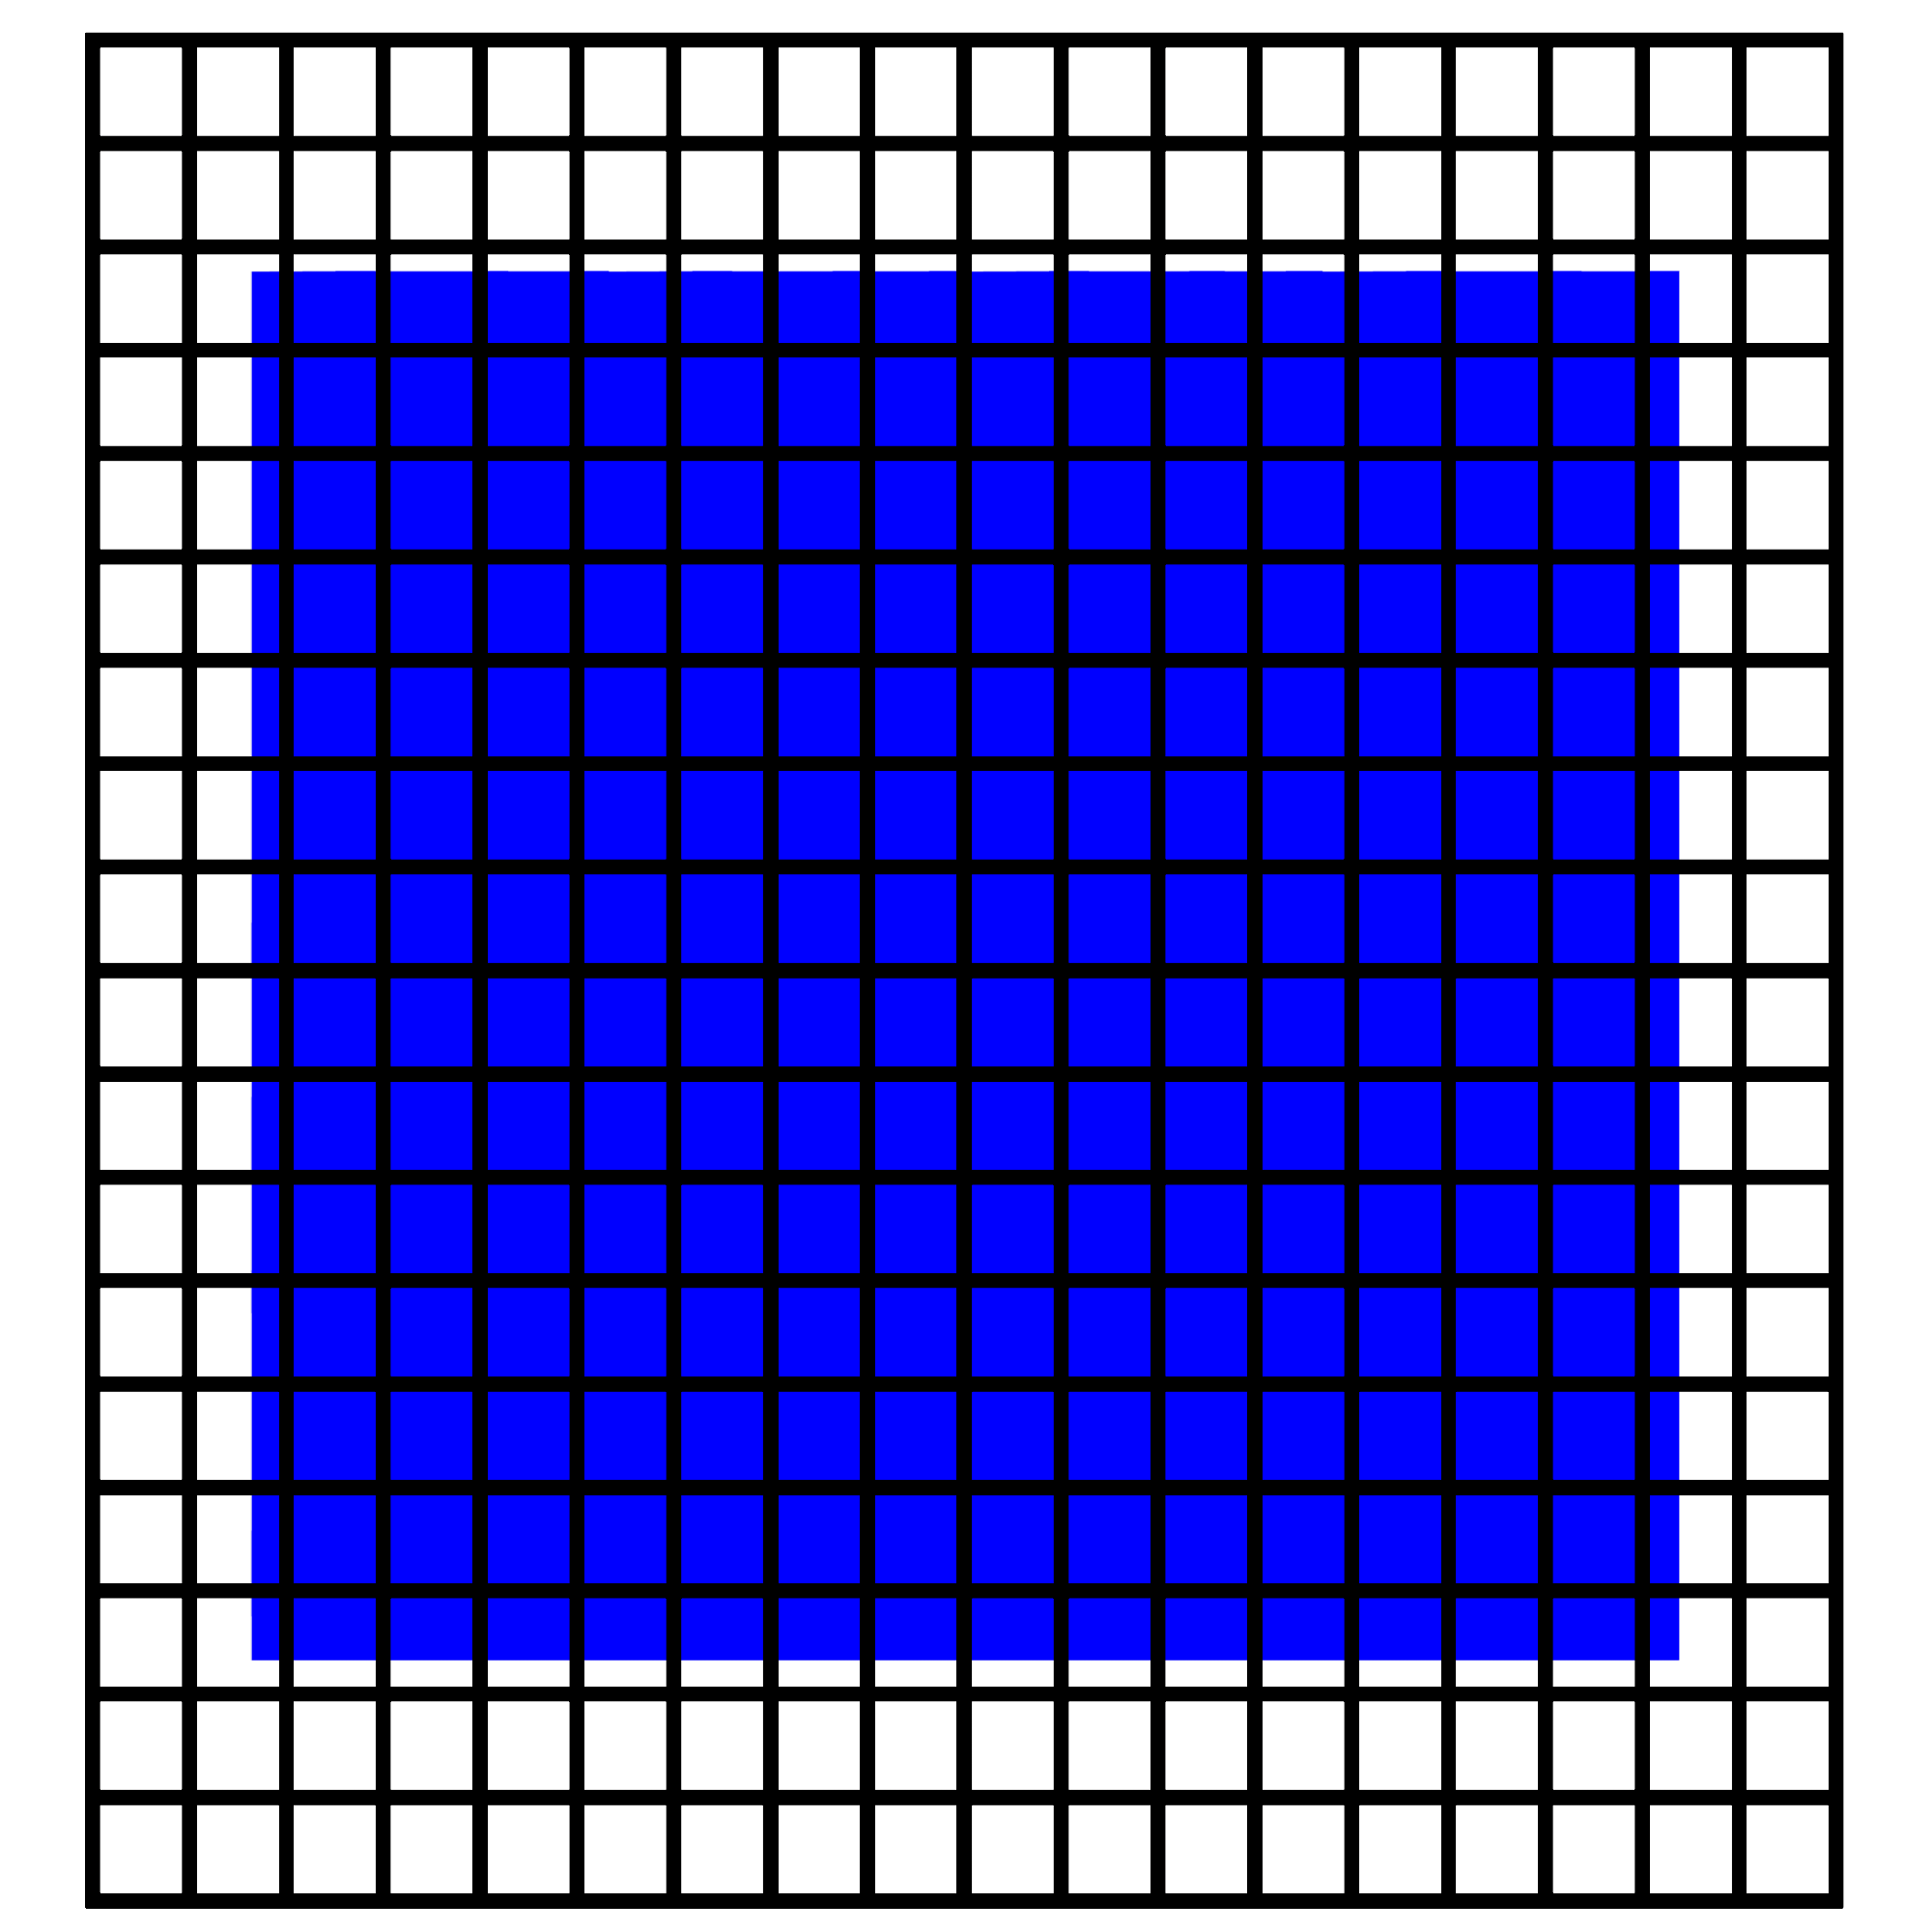
\includegraphics[width=0.4\textwidth]{Figures/eulerian_mesh_movement_001.png}
 &  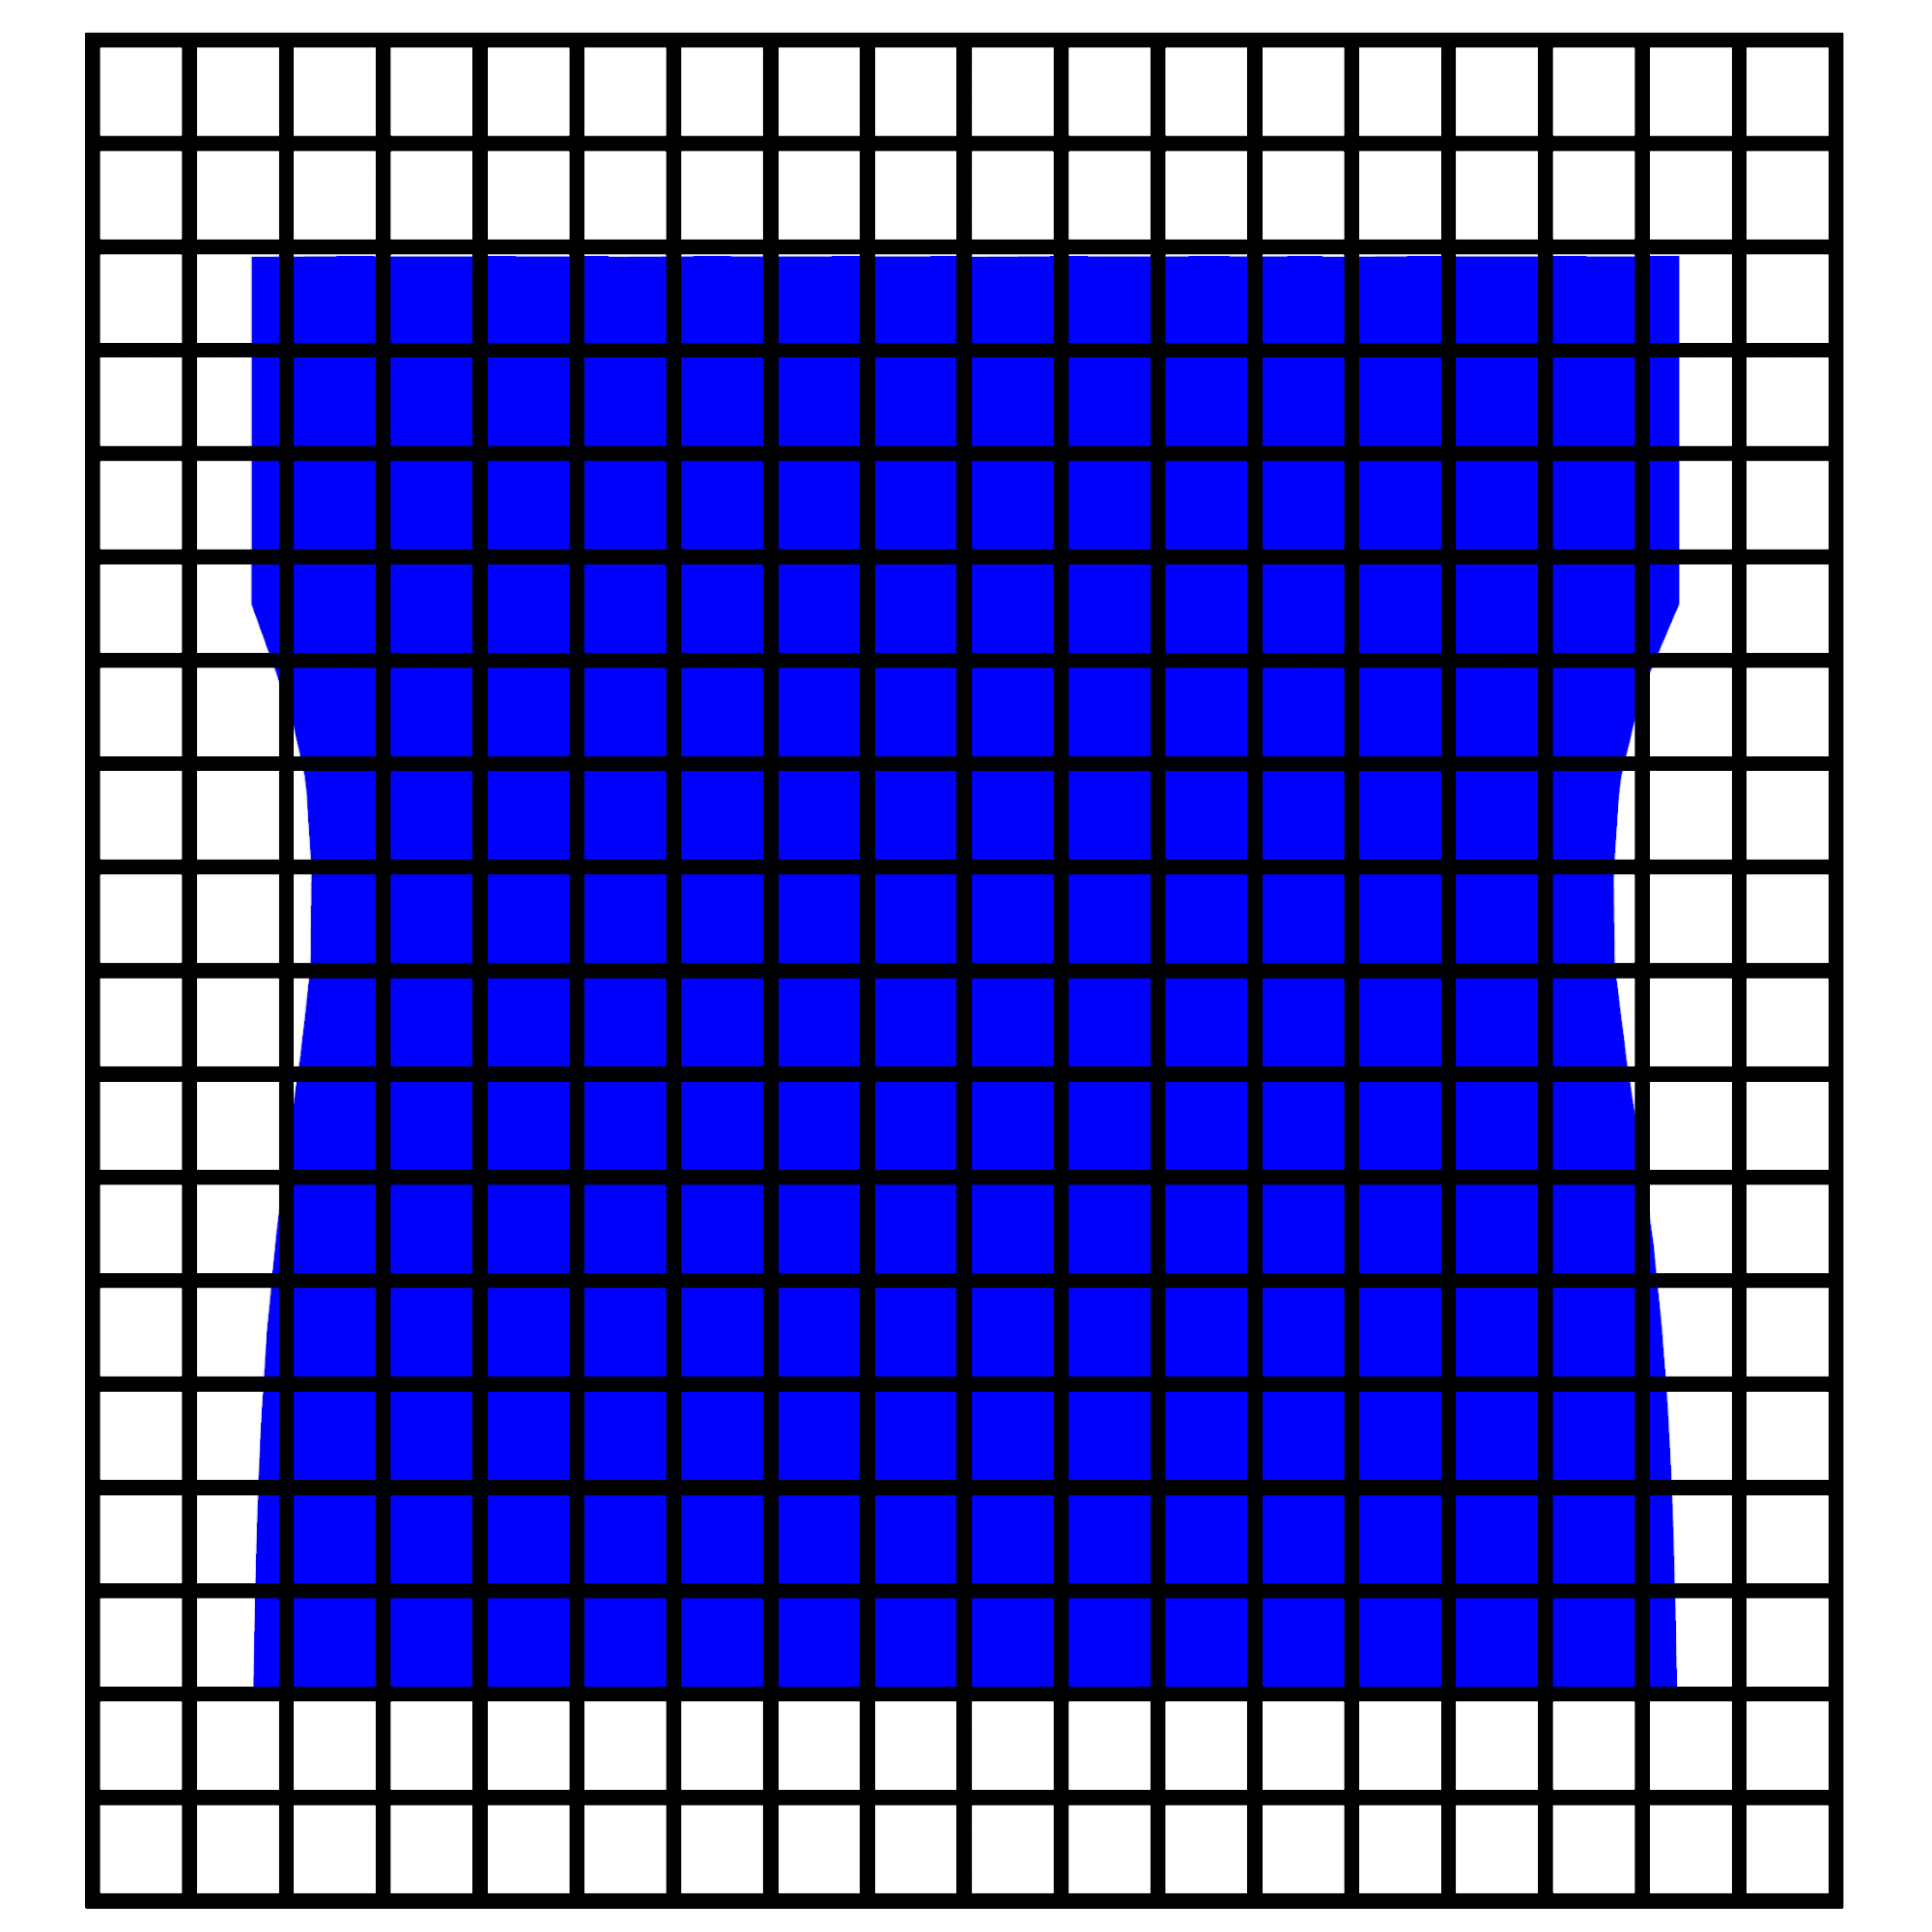
\includegraphics[width=0.4\textwidth]{Figures/eulerian_mesh_movement_002.png} 
 \\

	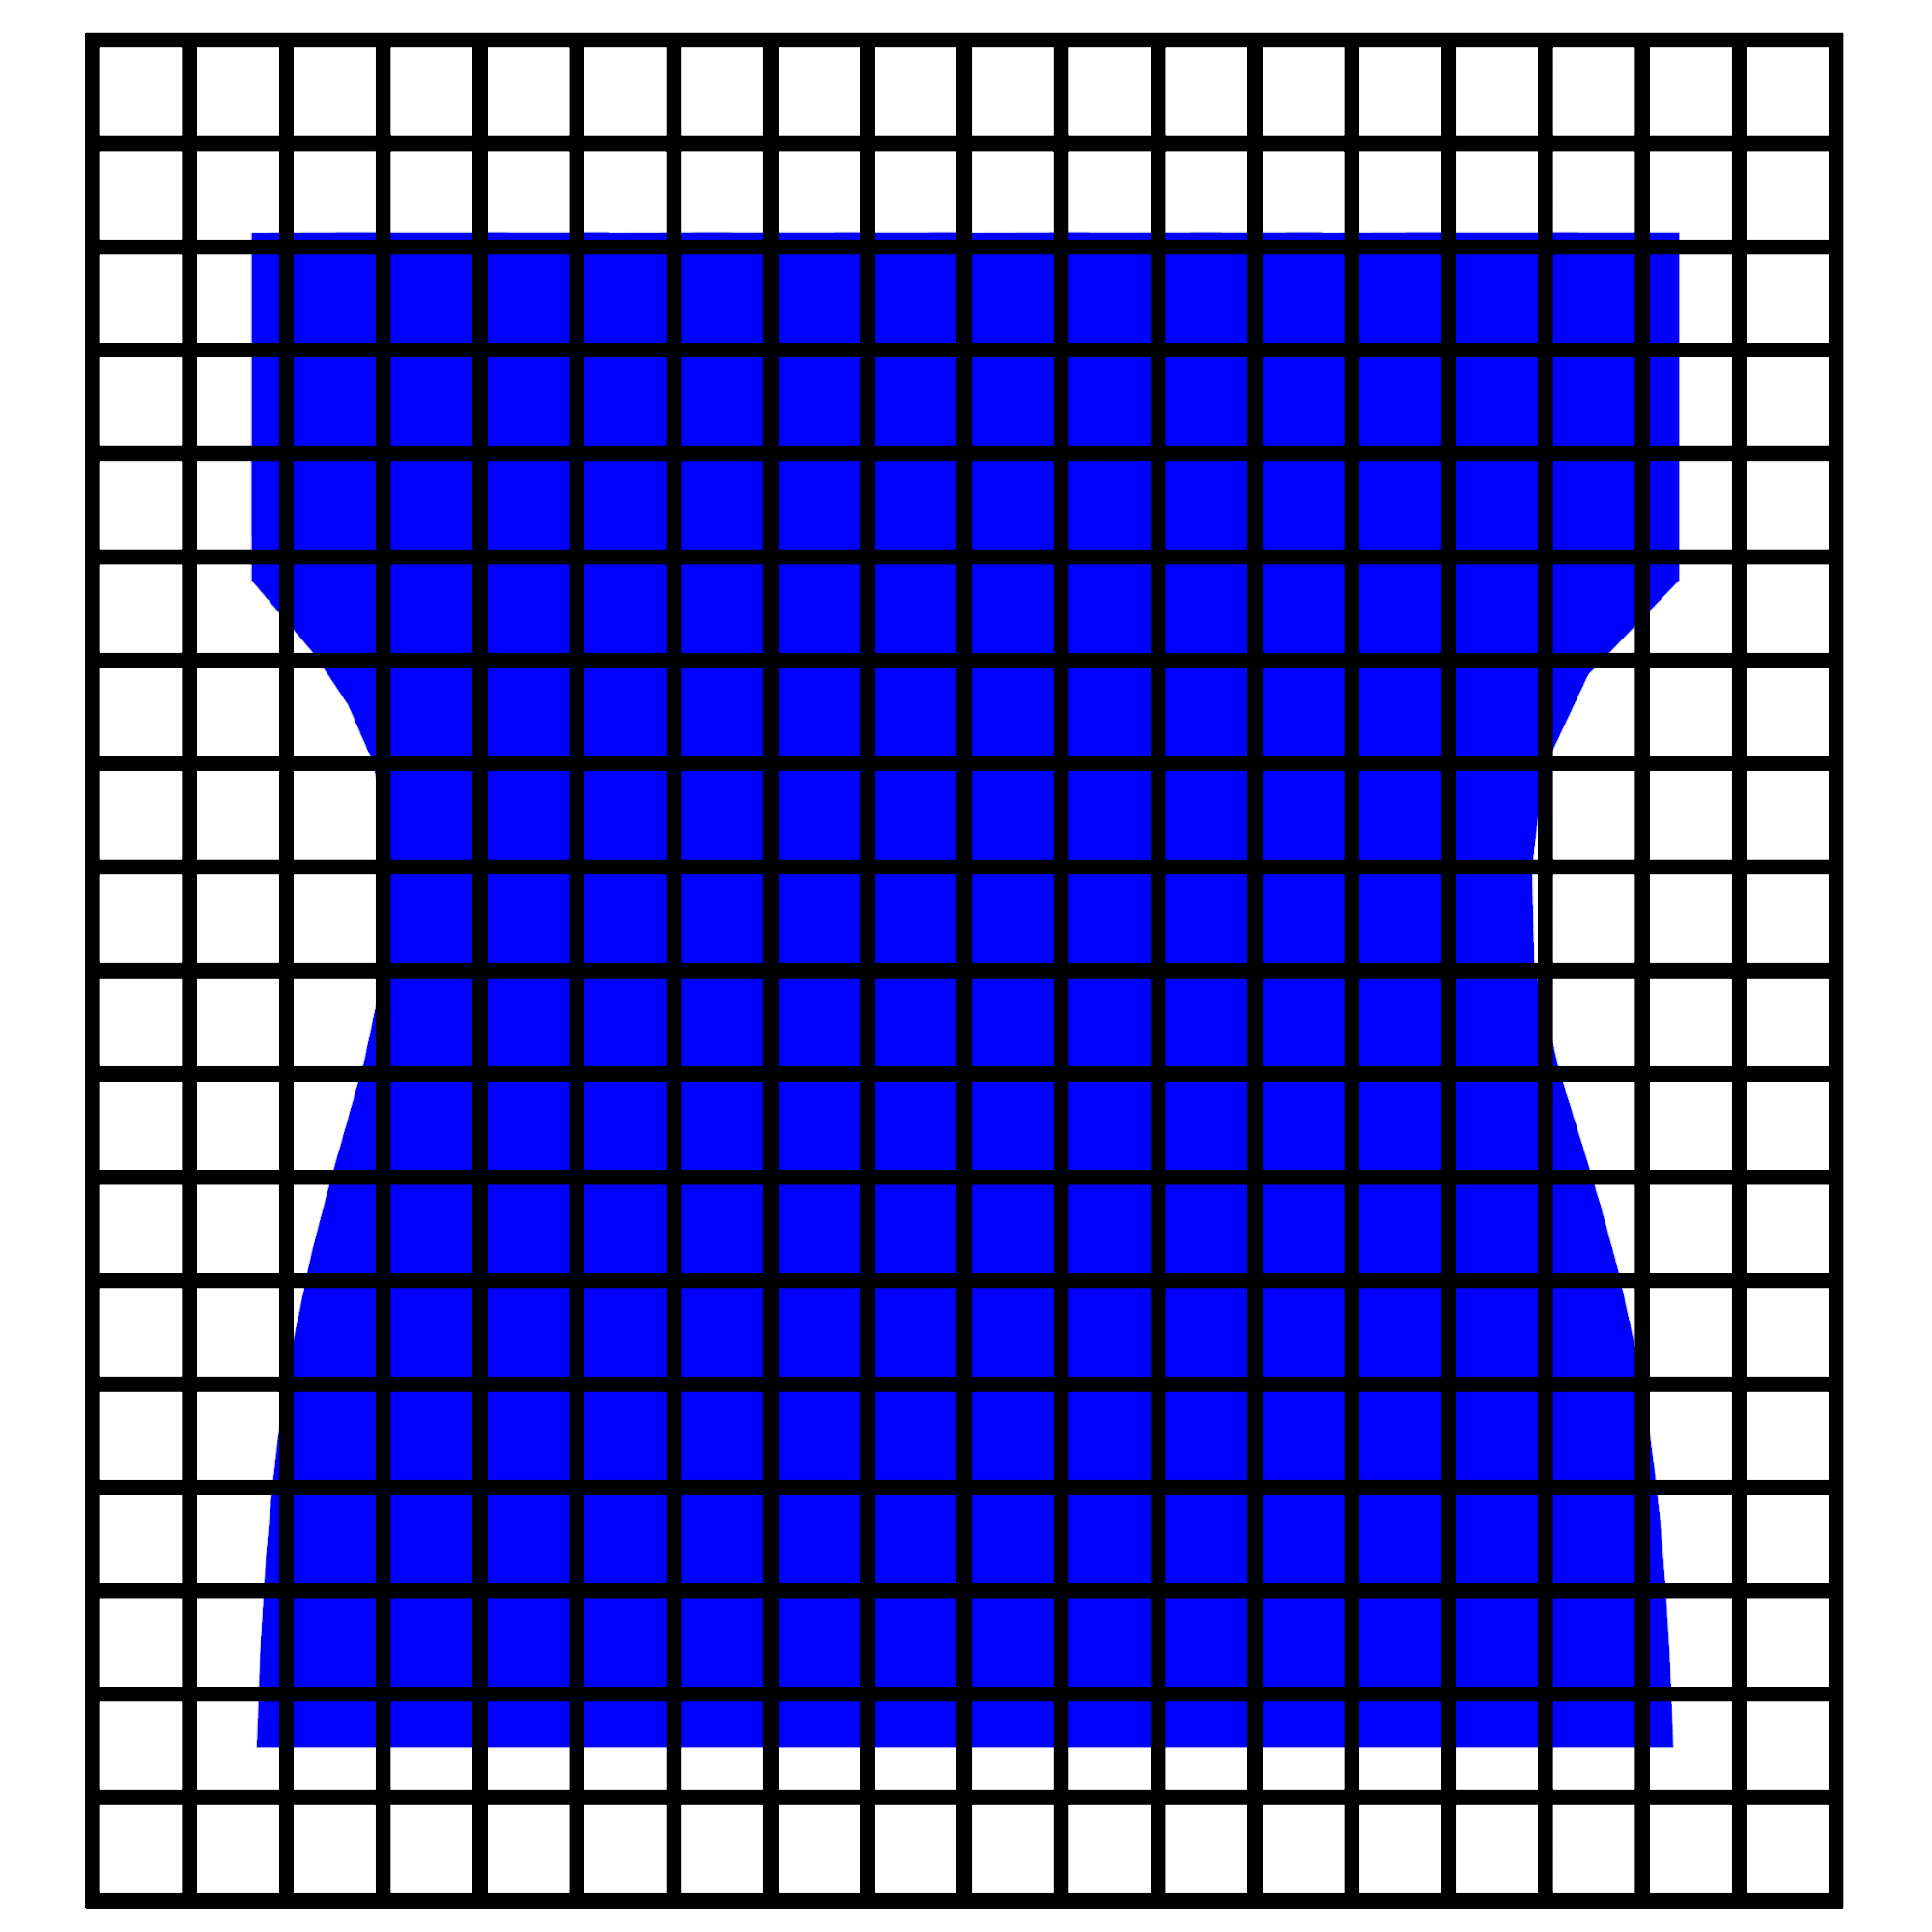
\includegraphics[width=0.4\textwidth]{Figures/eulerian_mesh_movement_003.png} 
 &  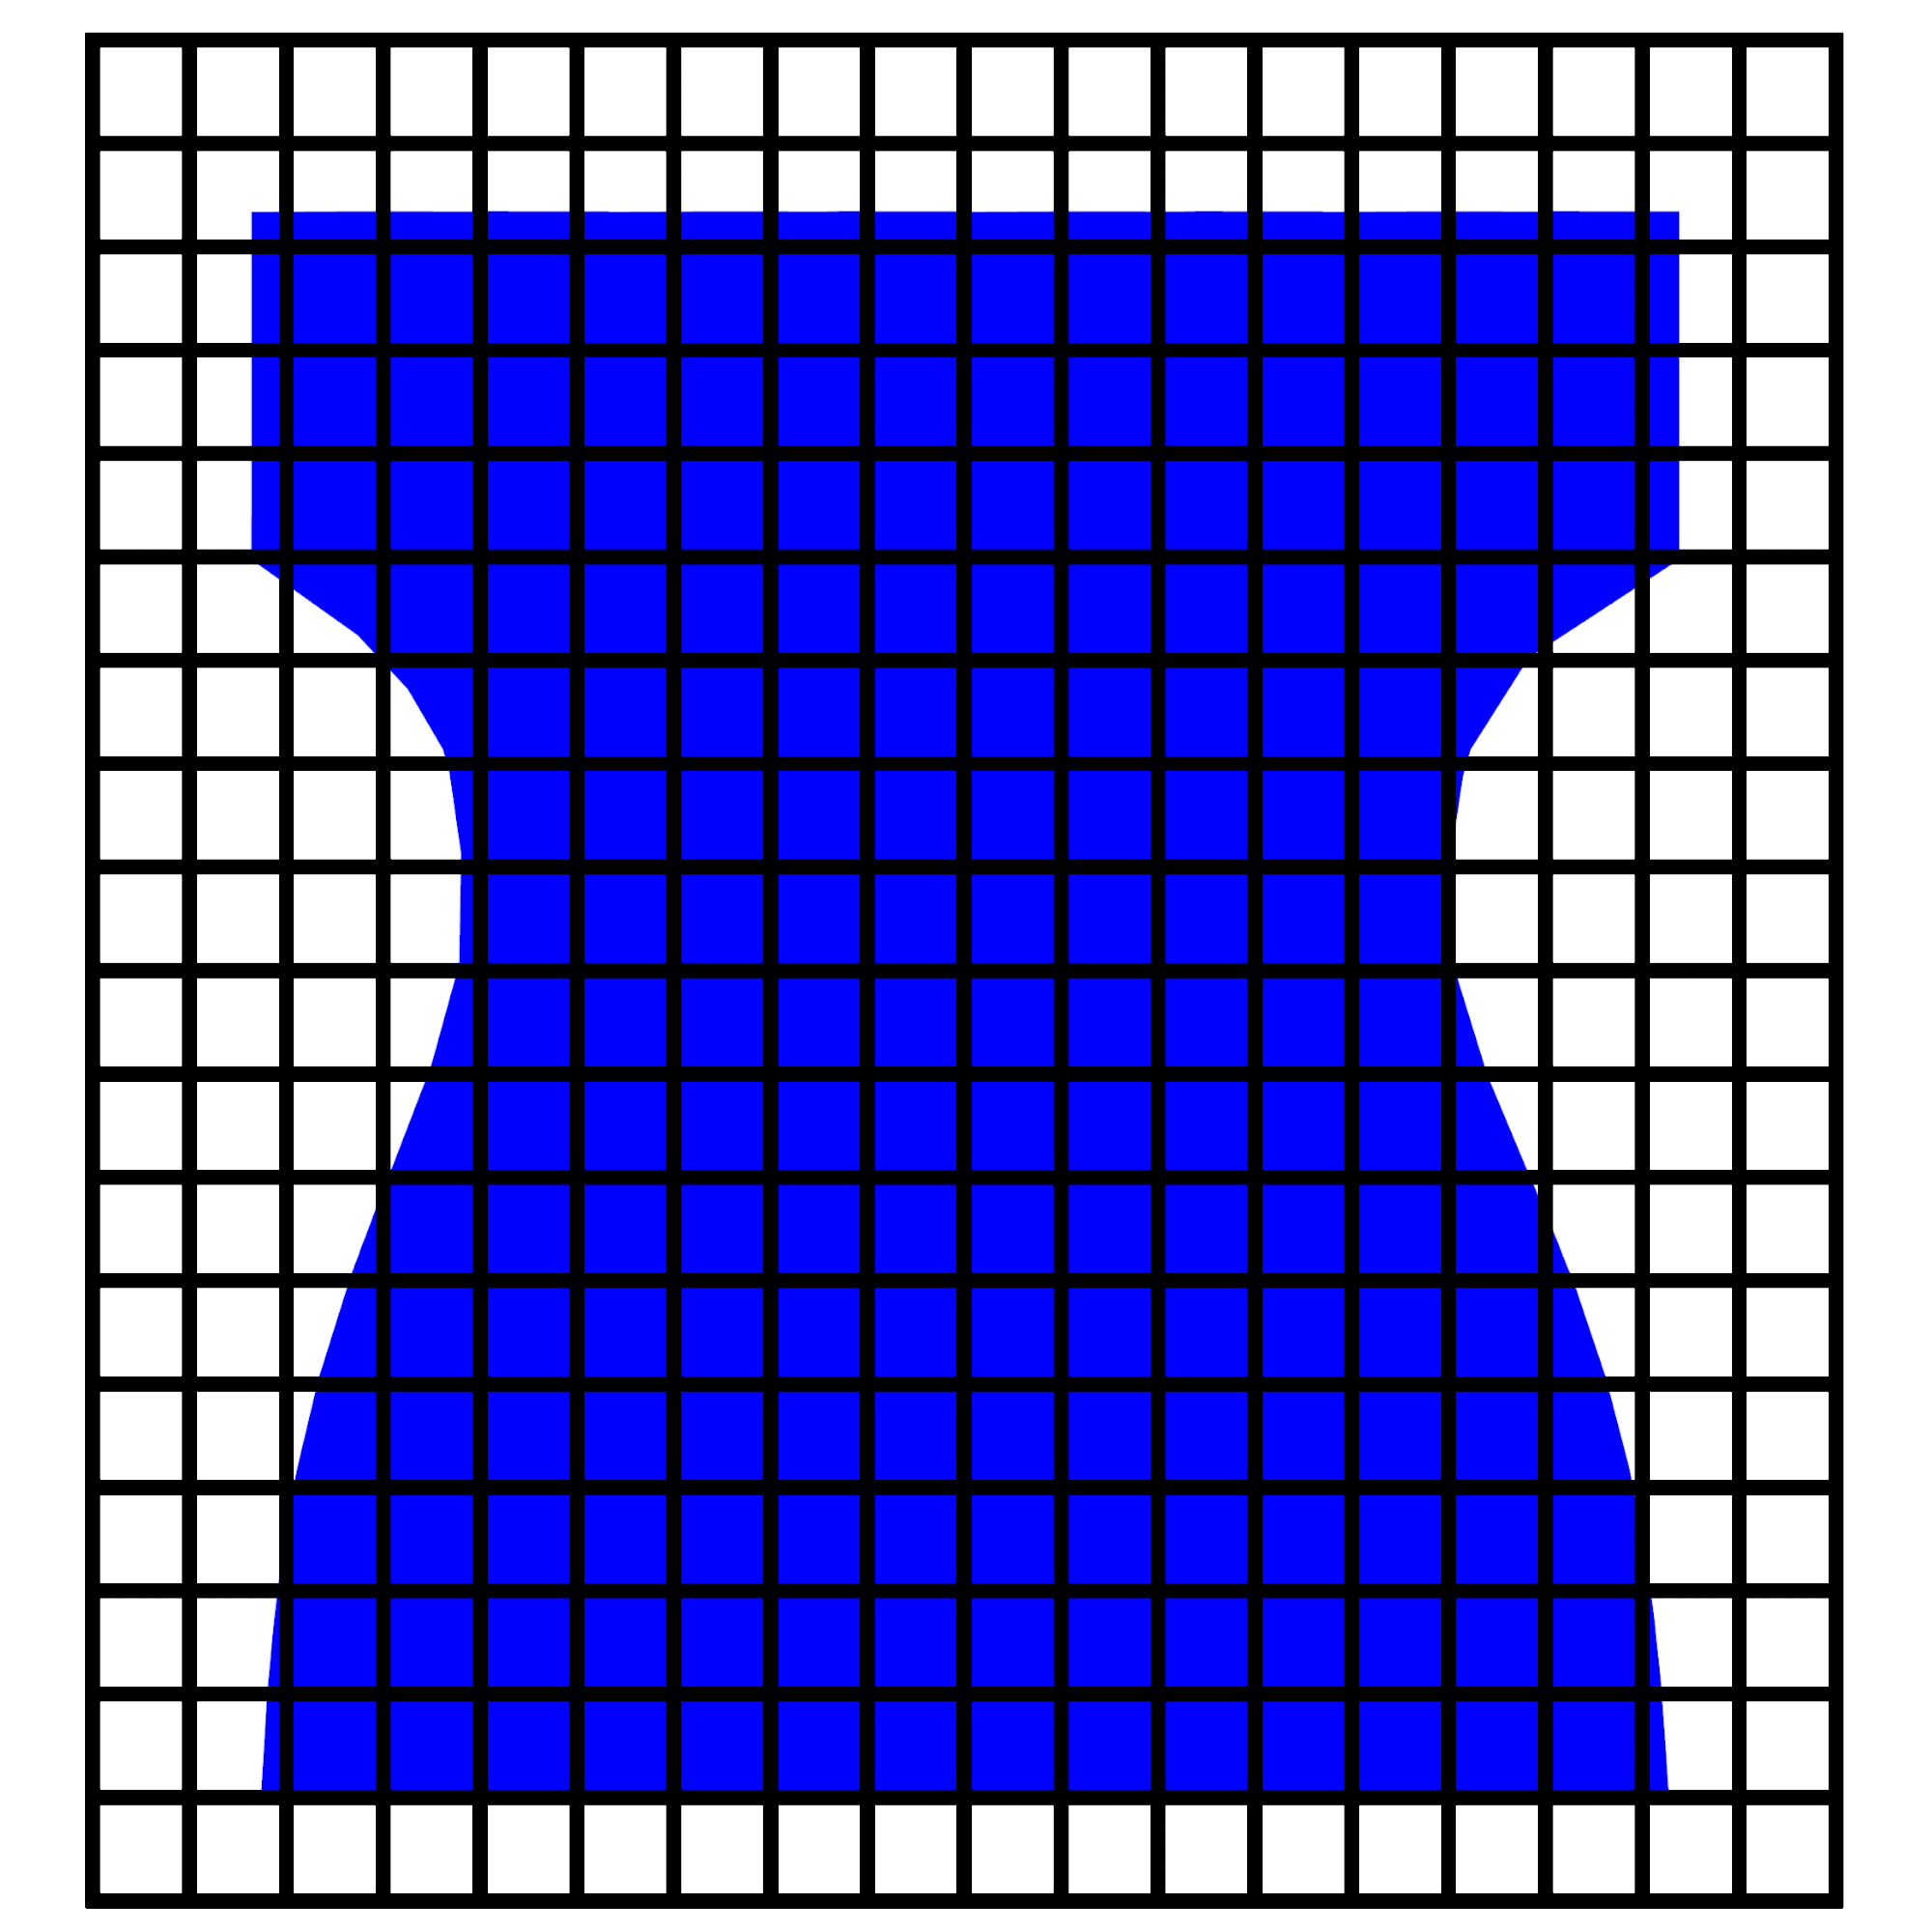
\includegraphics[width=0.4\textwidth]{Figures/eulerian_mesh_movement_004.png}  
 \\

\end{tabular}
\caption[bla]%
{Illustration of static Eulerian Mesh during material deformation \protect\footnotemark}
\label{fig:EulerMesh}
\end{figure}
\footnotetext{Illustration created in Autodesk Maya. This coarse mesh would not be sufficient enough to compute the detail of the deforming blue solid material.}


\subsection{Lagrangian Mesh}

The Lagrangian Mesh type is very similar to the Eulerian Mesh except that it incorporates the idea of the \nameref{sec:lagrangian_descr} into its spatial decomposition: A moving reference system. The mesh itself is clamped to the material and will deform and move accordingly as the material itself. Figure \ref{fig:LagMesh}
demonstrates such a deformation, in which a stretch behaviour is simulated. The mesh is \emph{body-fitted} to the actual geometry that deforms. In constrast to a Eulerian meshes we can cleary see how the triangular elements of the material deform from the left upper picture to the right lower picture during the simulation. This type of mesh is used in the Finite Element Method for CSM and CFD and has various
advantages over Eulerian Meshes, which will be discussed in Chapter \ref{sec:adv_of_fem}. However combining a mesh with the Lagrangian perspective also leads to problems
like \nameref{sec:remeshing_fem}. These problems can be overcome by discarding the concept of a mesh description for discretization and creating a meshfree and purer Lagrangian discretization concept with freely moving particles, which is done in Chapter \ref{Chapter 5}. For further reading please refer to \citep{Bennett2006}.


\begin{figure}[htb]
\centering
\begin{tabular}{cc}
	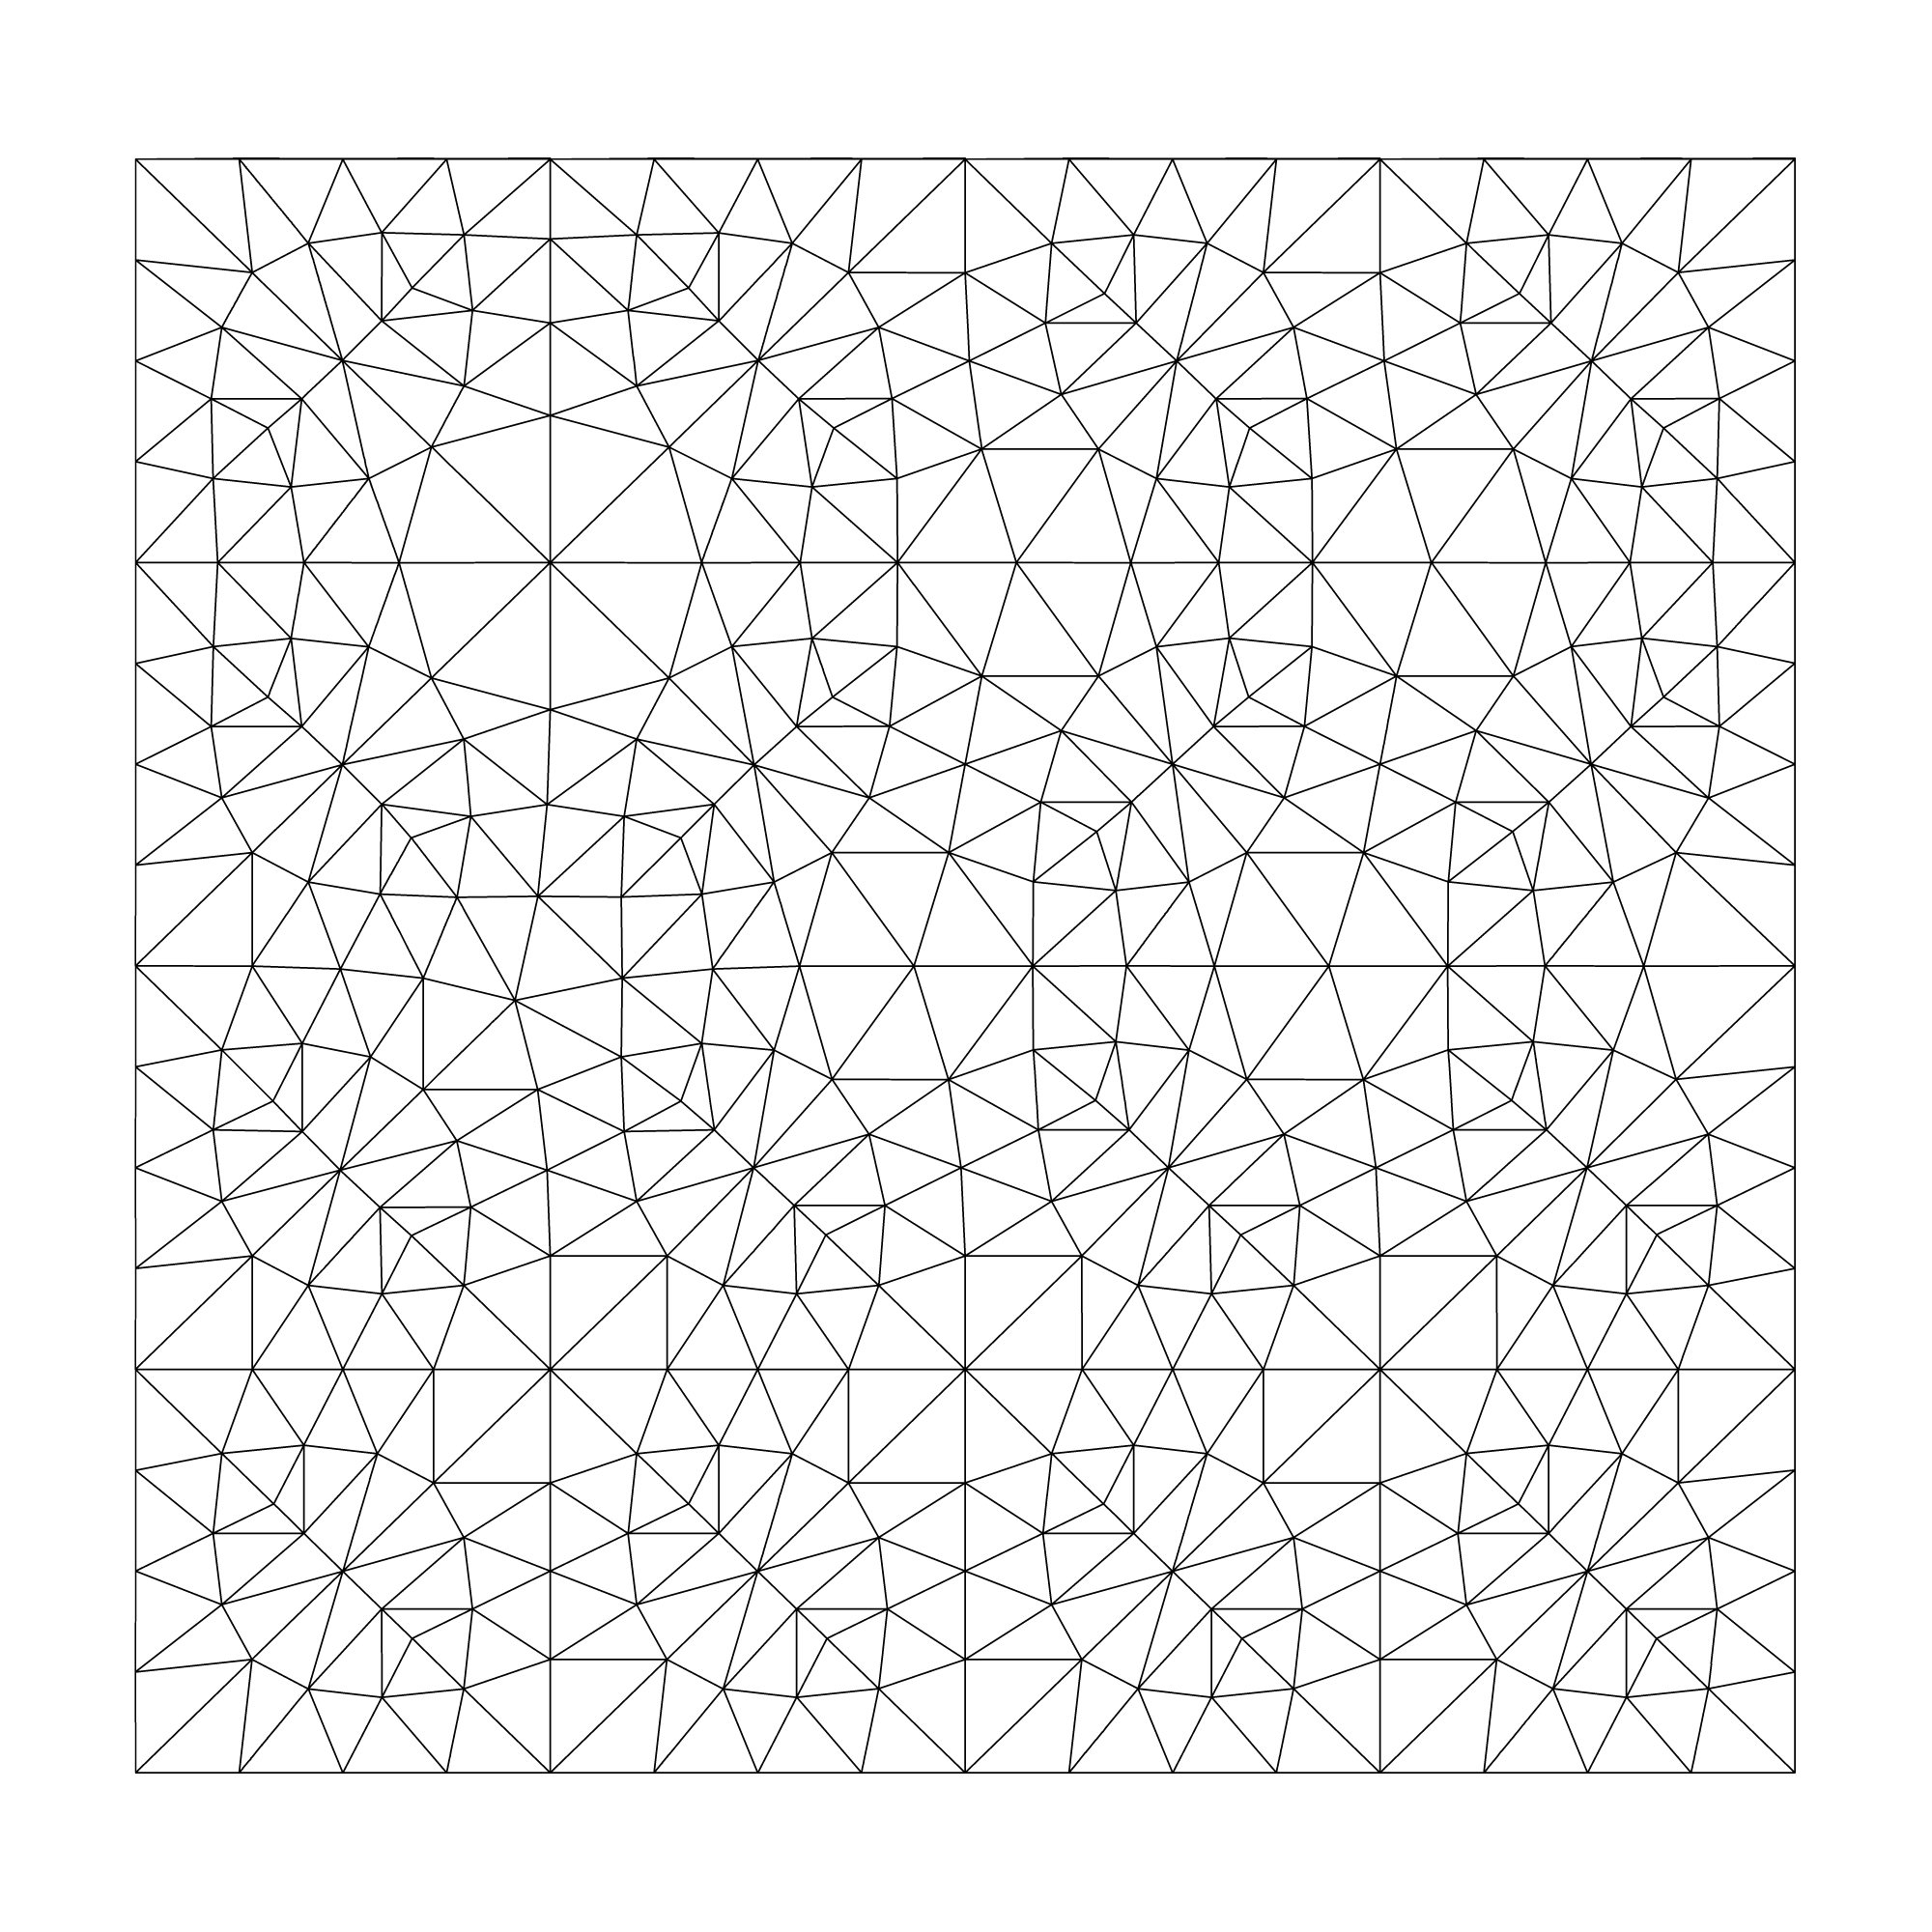
\includegraphics[width=0.4\textwidth]{Figures/lagrangian_mesh_movement_001.png}
 &  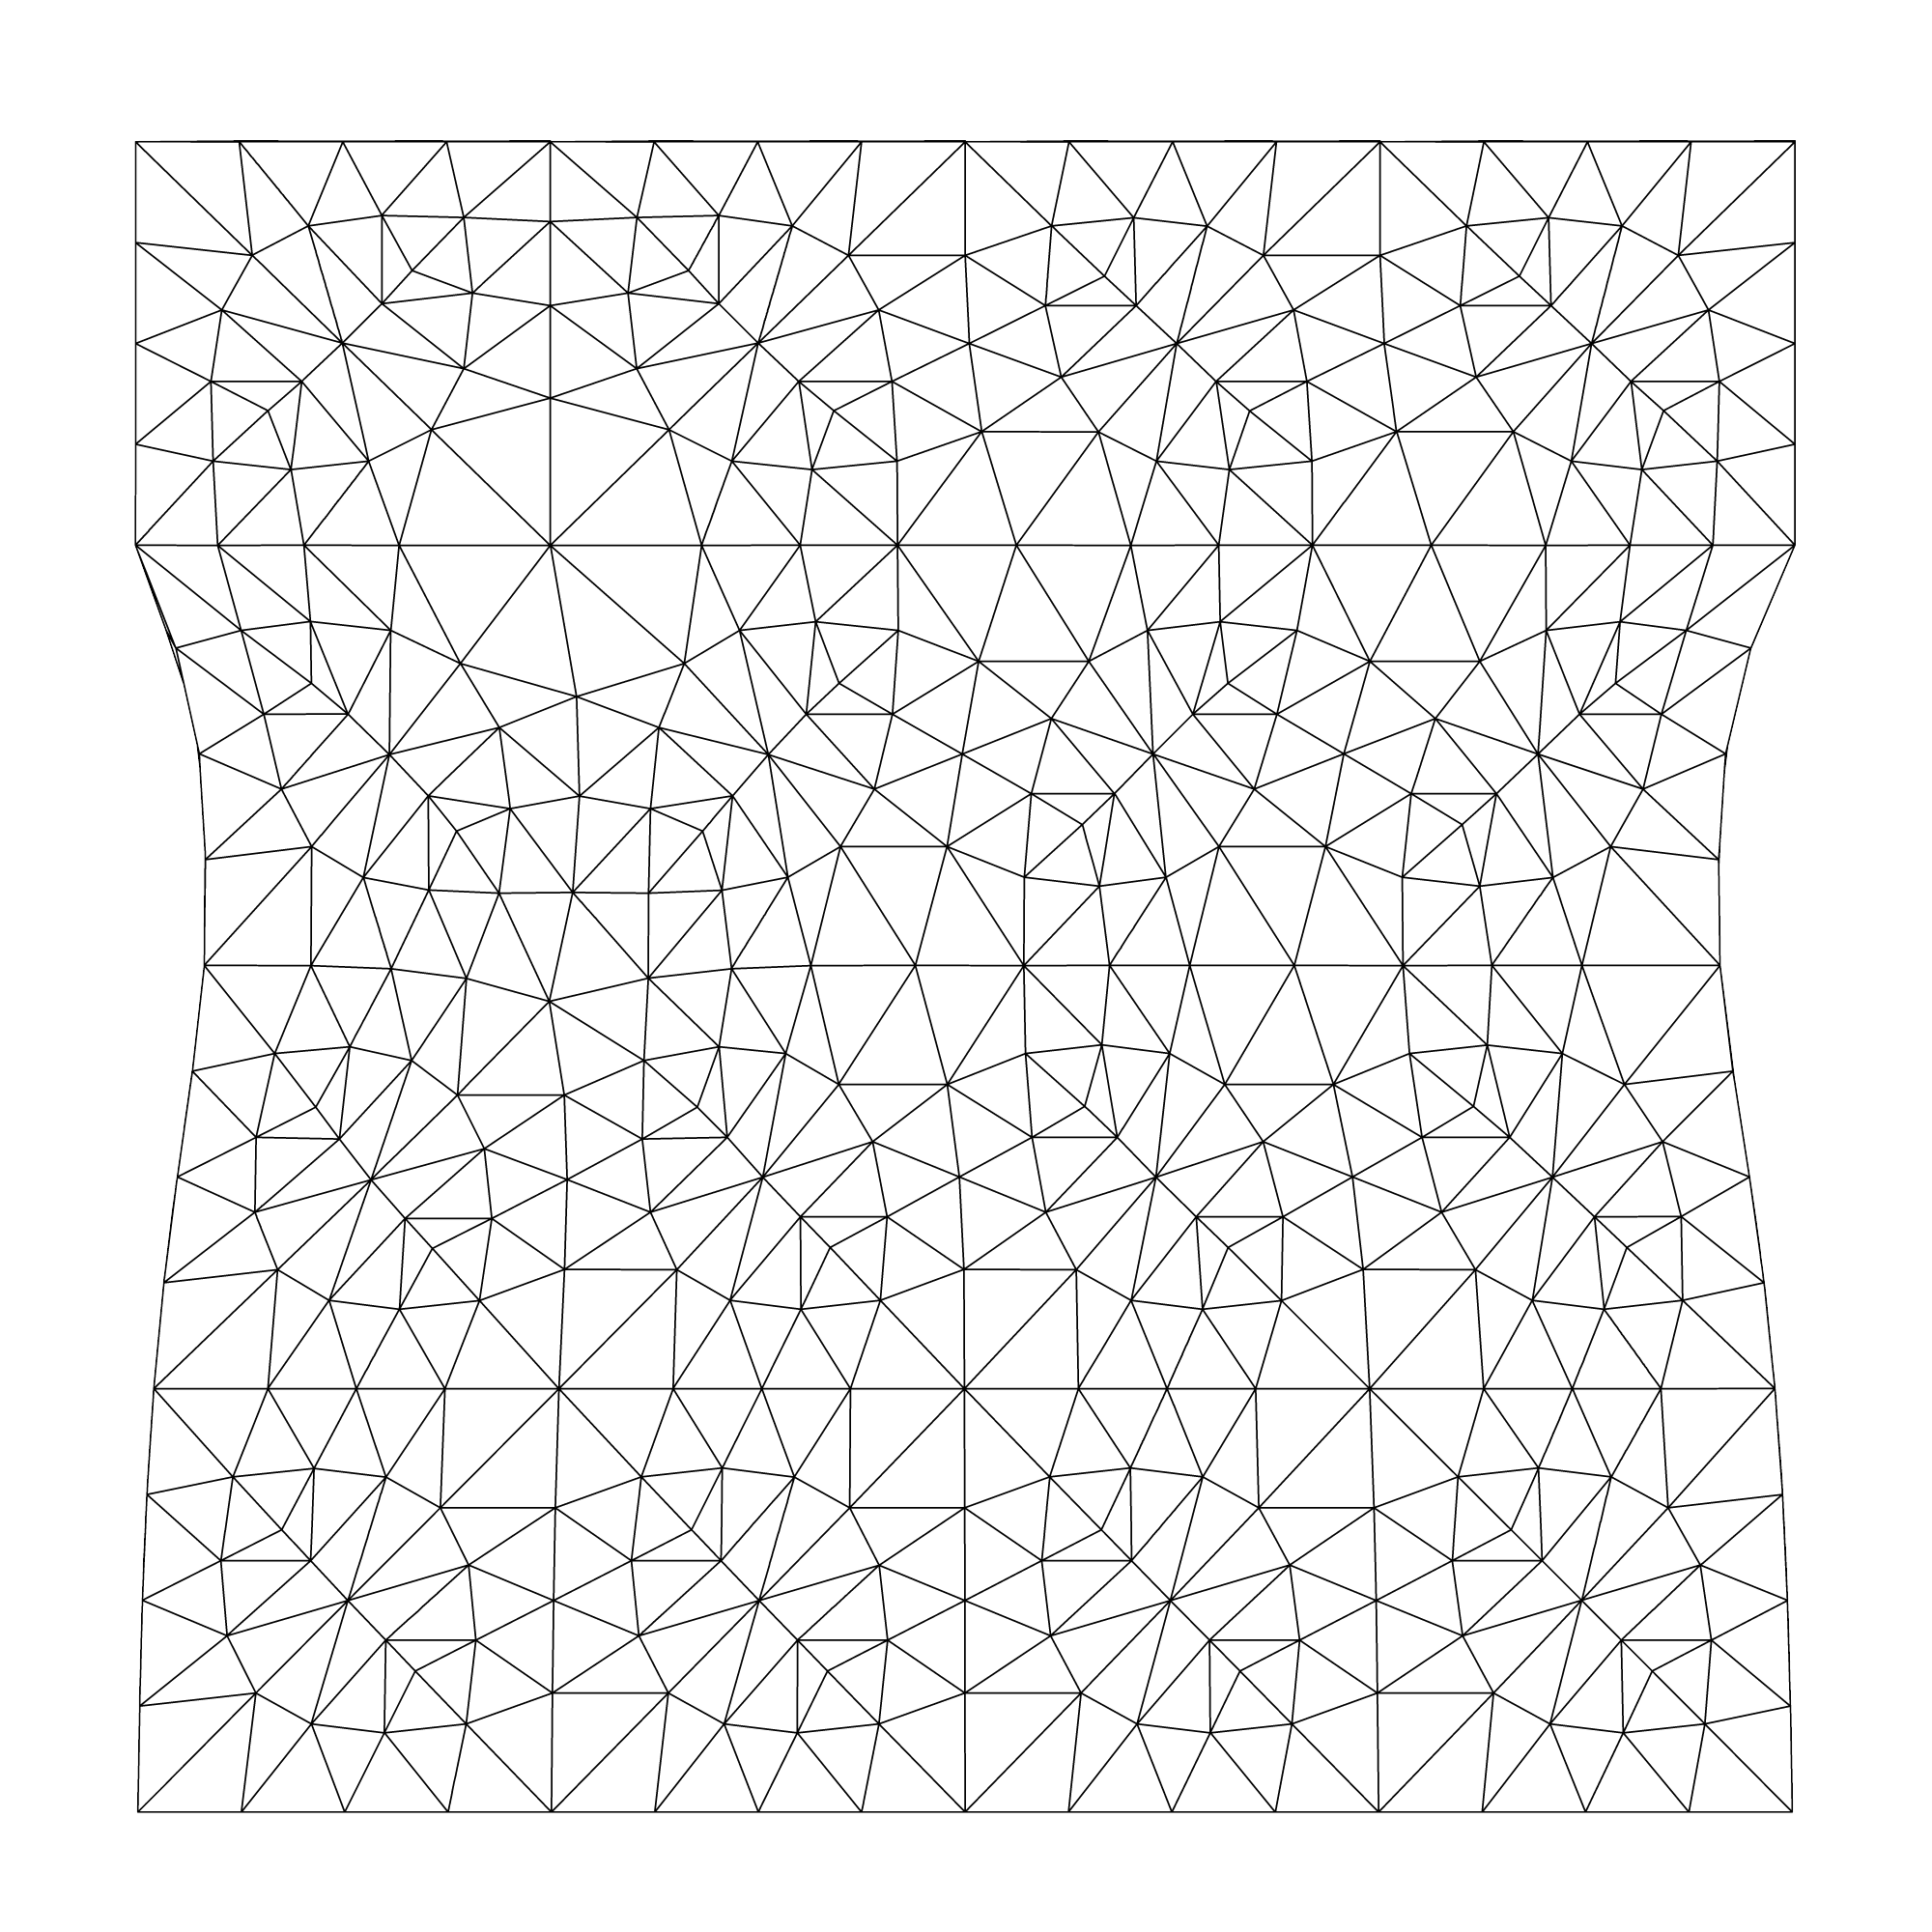
\includegraphics[width=0.4\textwidth]{Figures/lagrangian_mesh_movement_002.png} 
 \\

	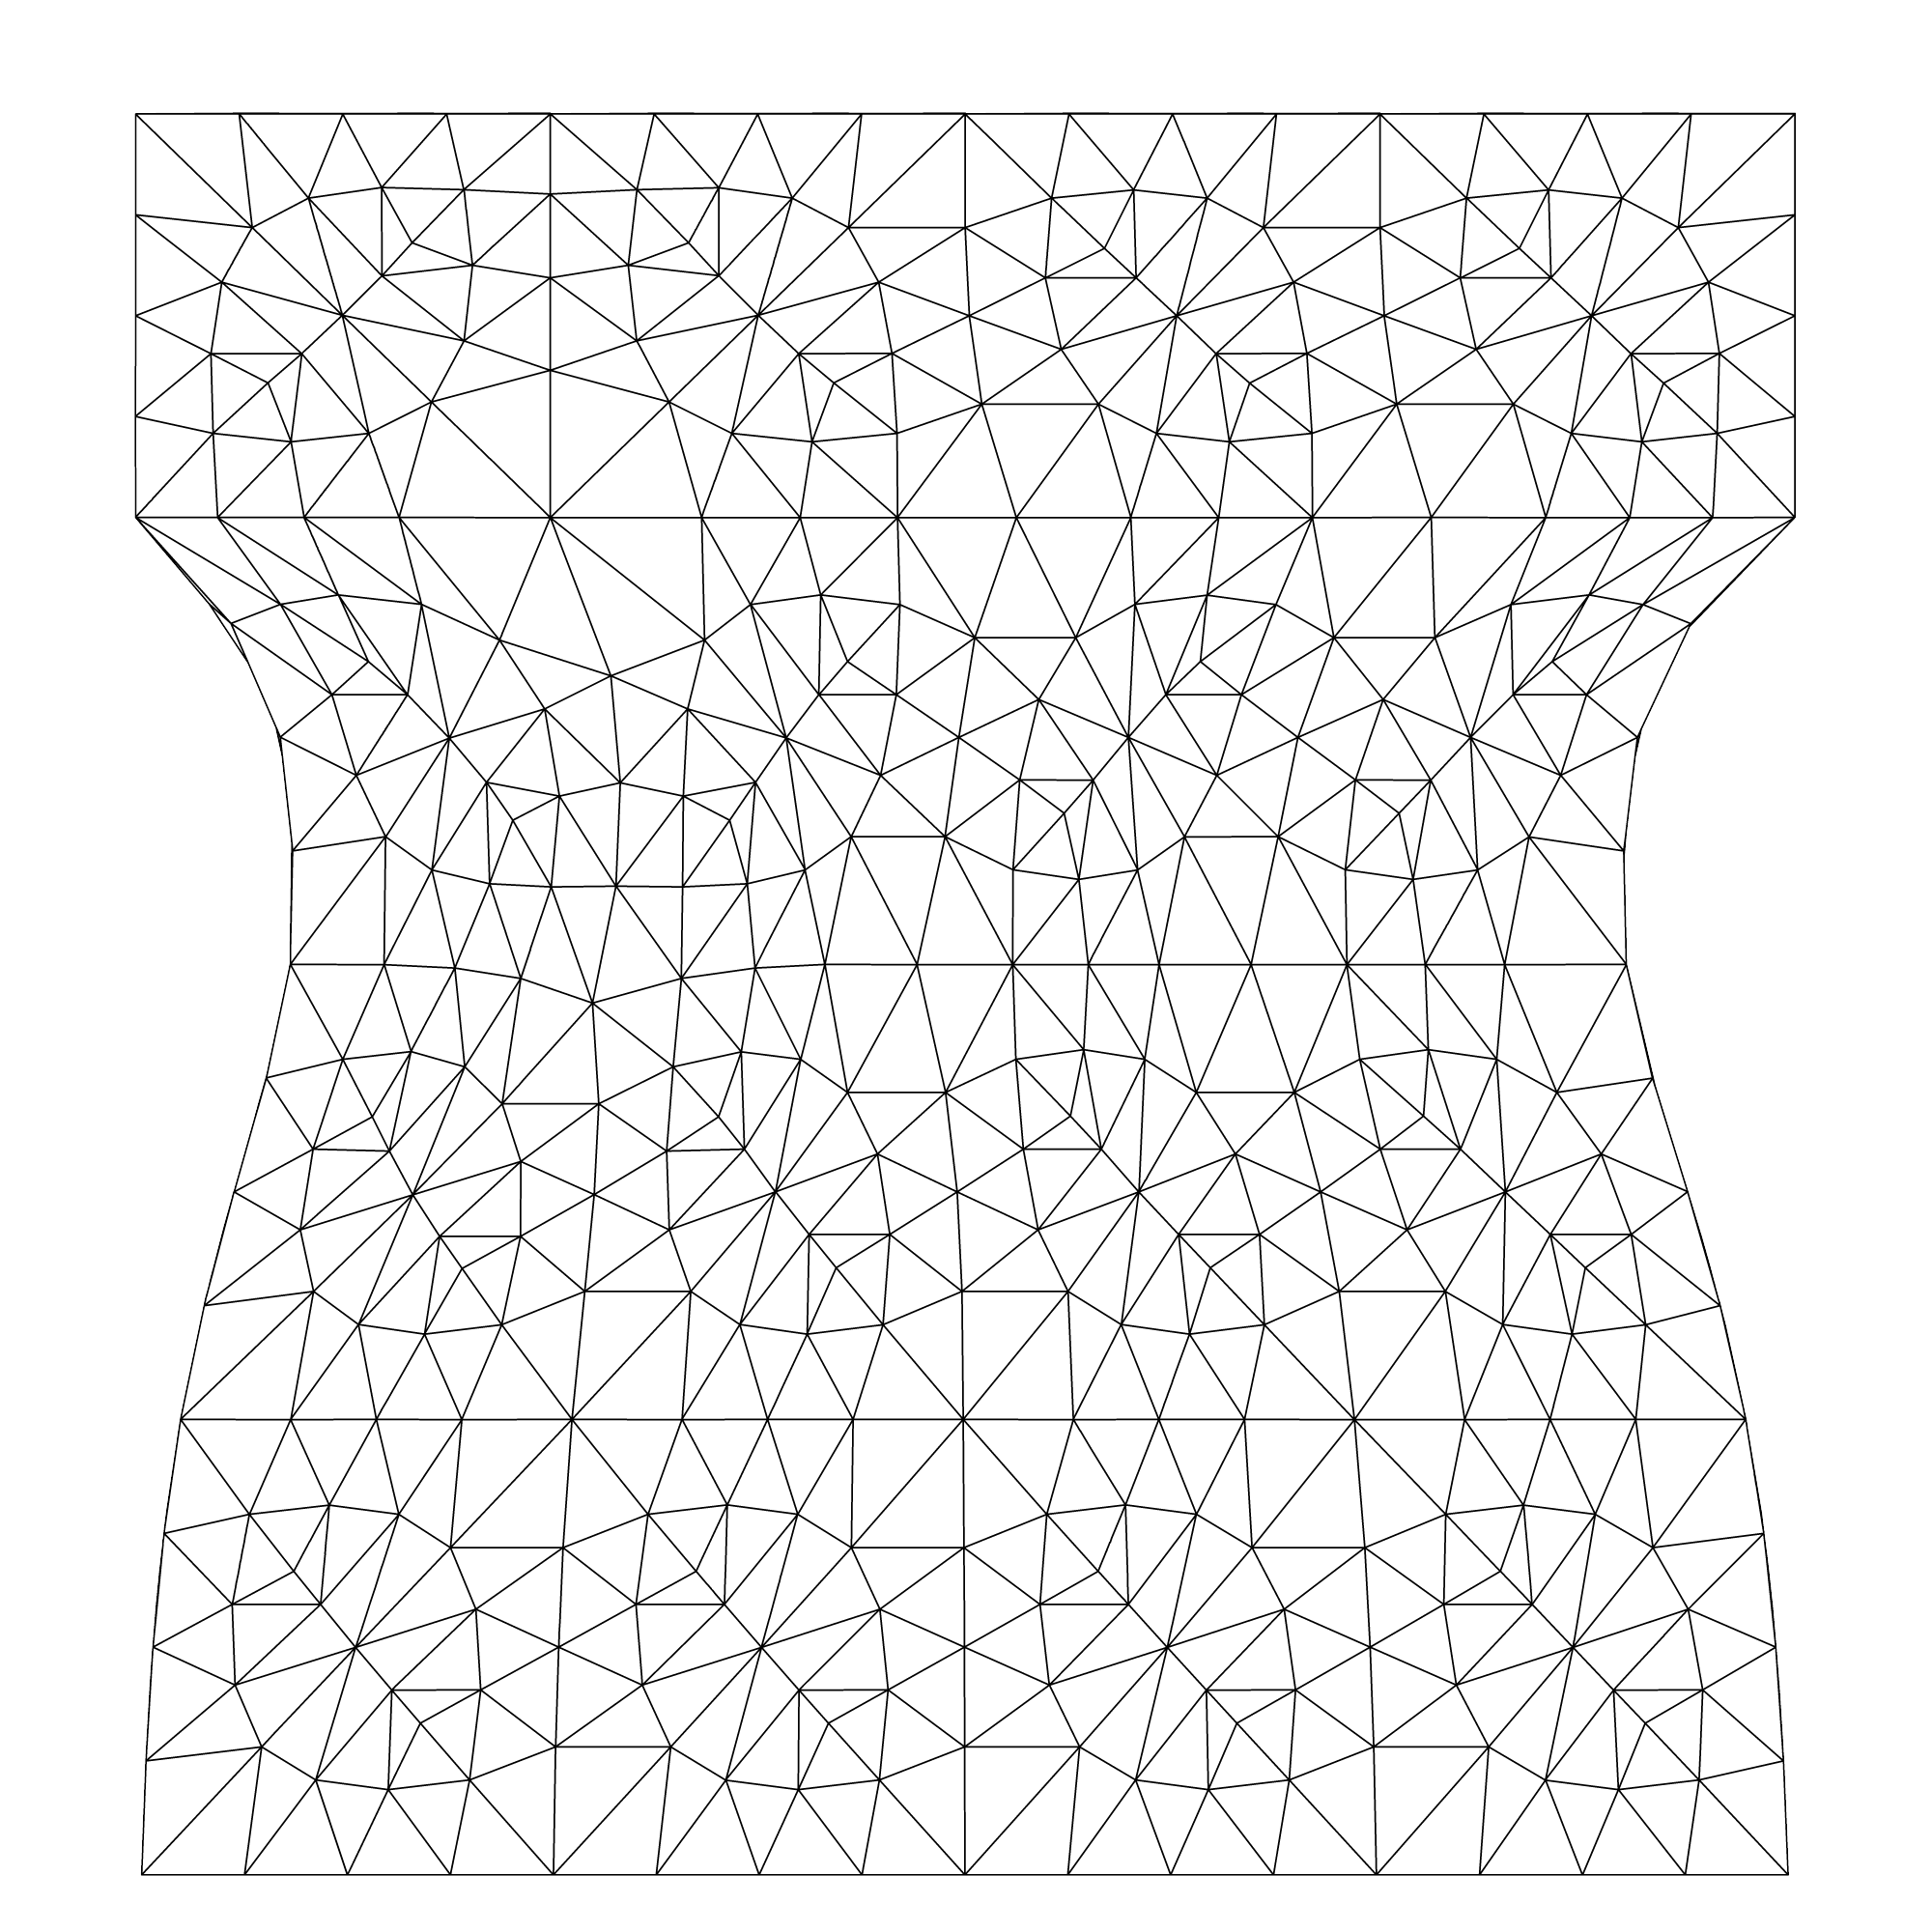
\includegraphics[width=0.4\textwidth]{Figures/lagrangian_mesh_movement_003.png} 
 &  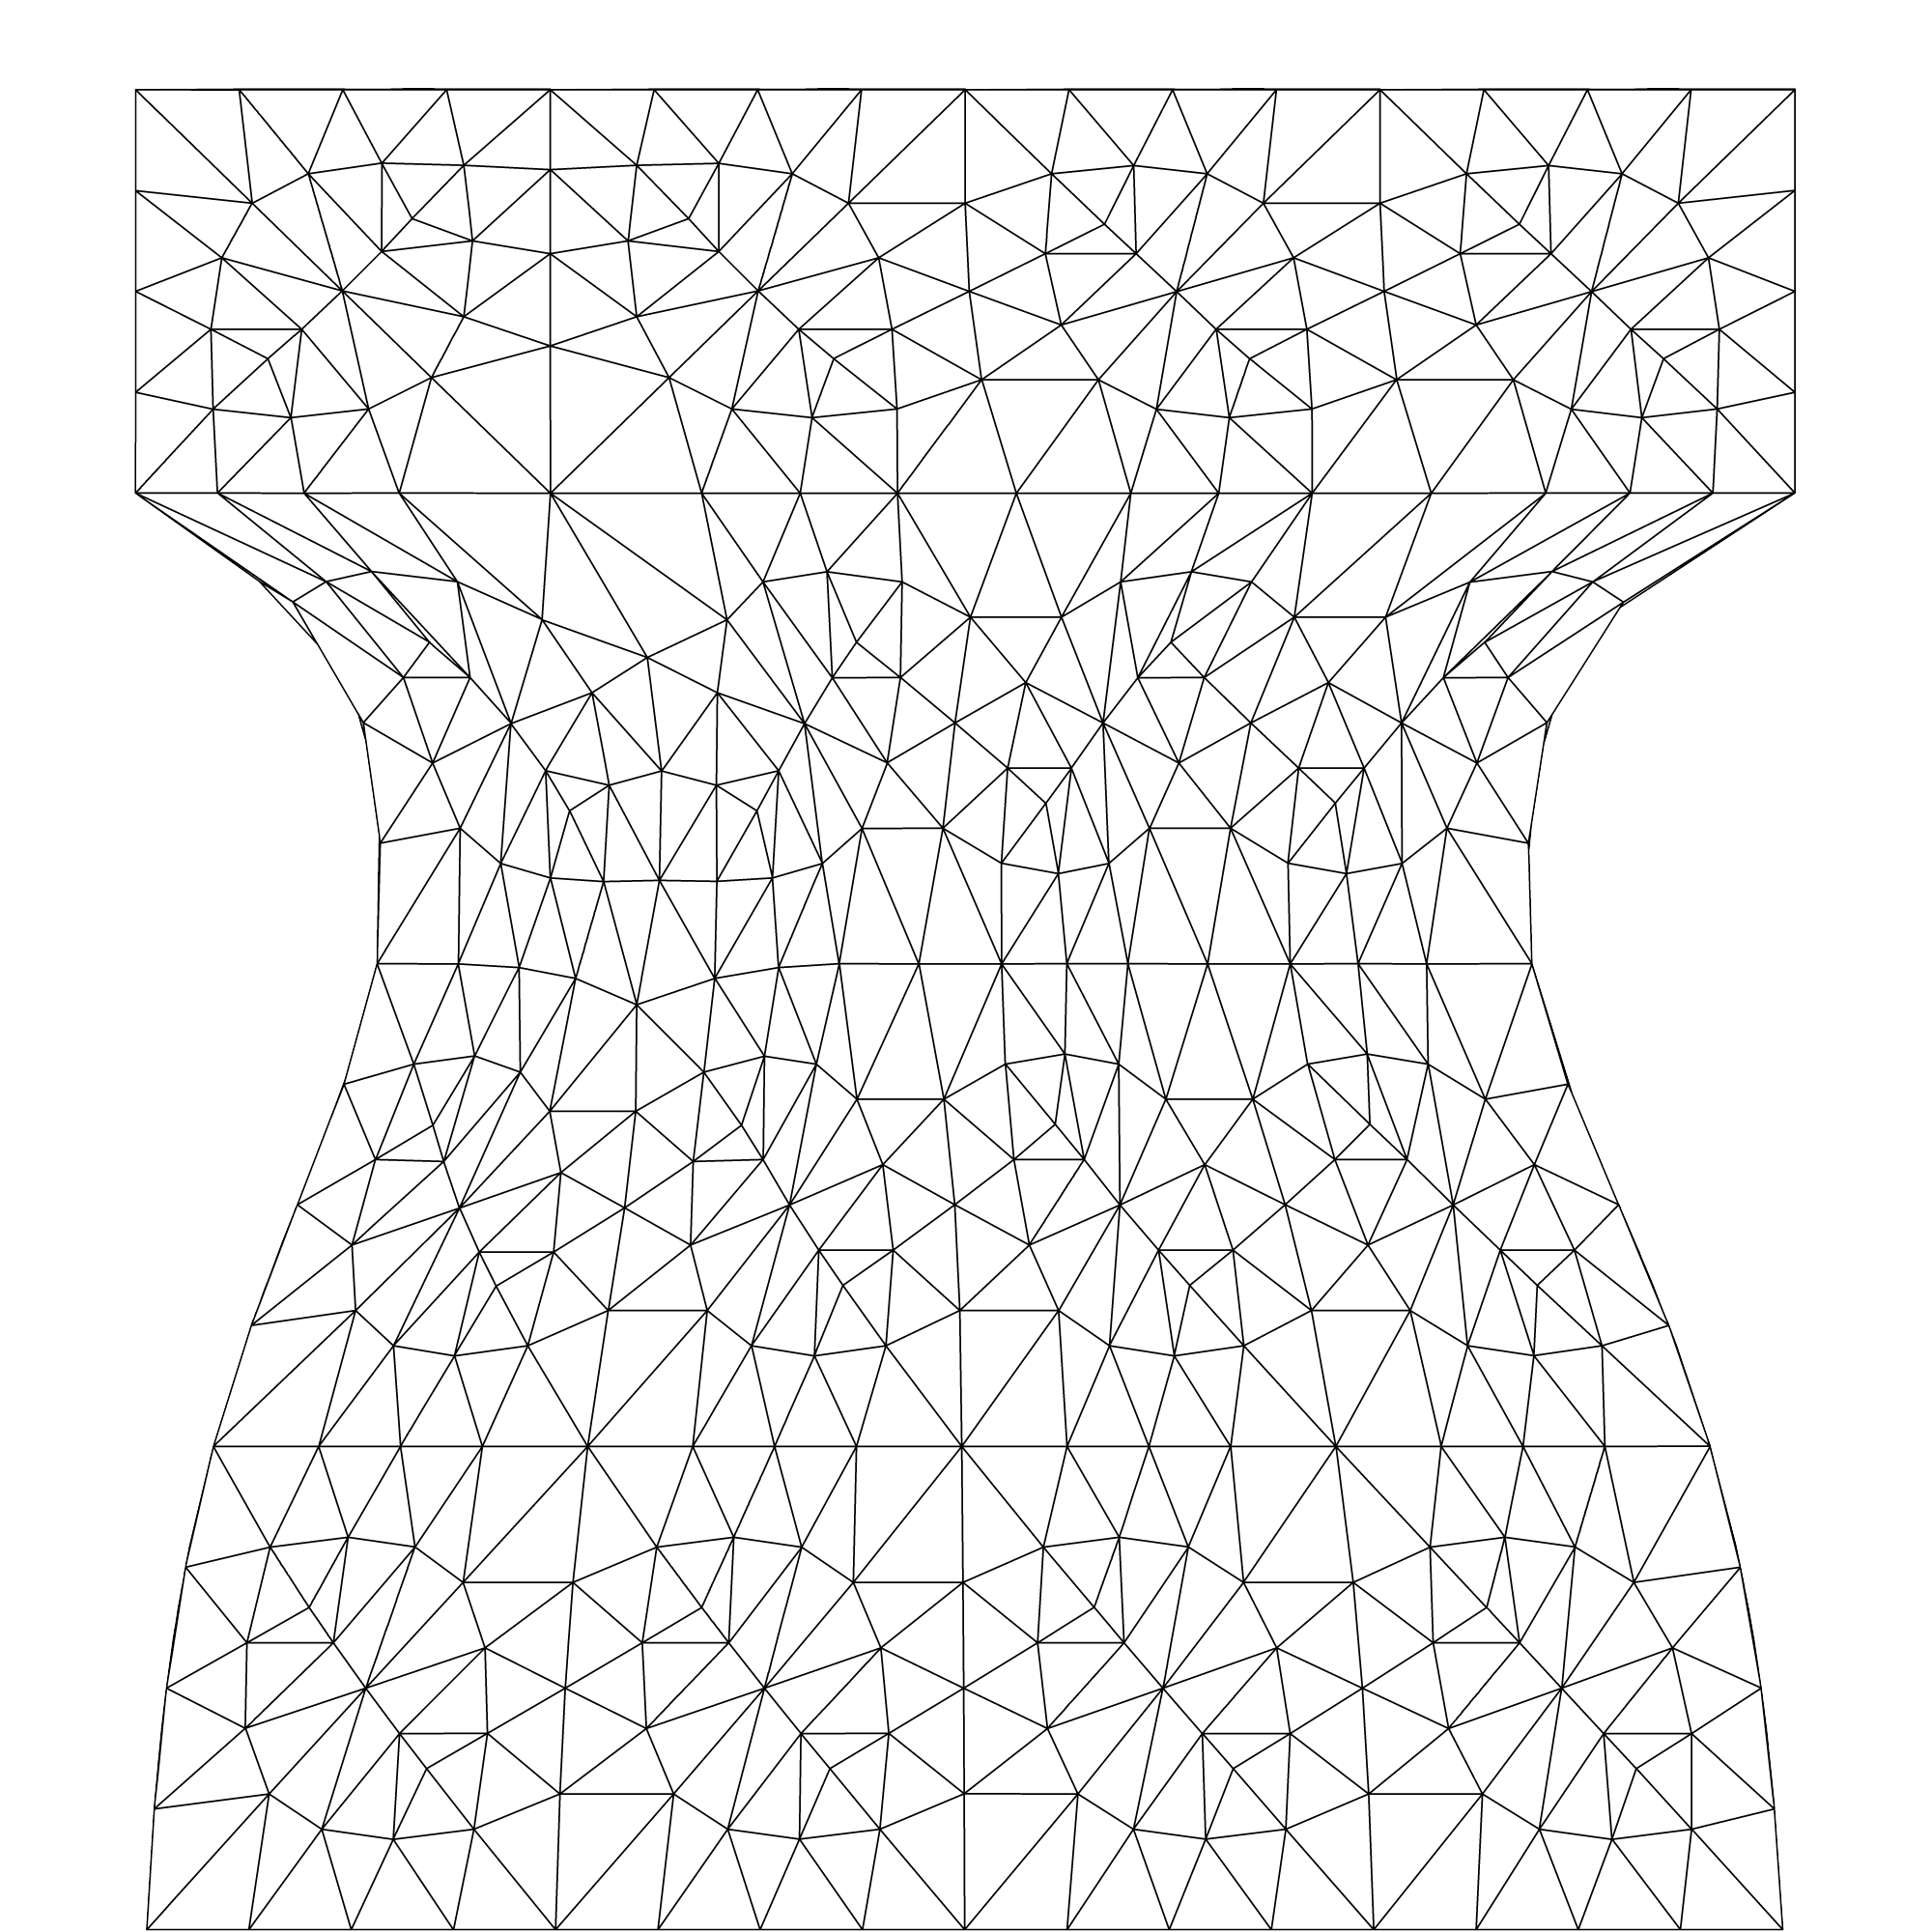
\includegraphics[width=0.4\textwidth]{Figures/lagrangian_mesh_movement_004.png}  
 \\

\end{tabular}
\caption[bla]%
{Movement of Lagrangian Mesh  during deformation \protect\footnotemark}
\label{fig:LagMesh}
\end{figure}
\footnotetext{Created in Ansys.}


\section{Further Reading}
Alongside the already given literature in this Chapter, \citep{Wohlmuth2001} and \citep{Hirsch2007} give a in-depth view into discretization.

\section{Chapter passage}
With the now established general knowledge of spatial discretization and mesh types, the following Chapters
will describe the actual discretization methods and the mathematical details behind them.

% Chapter Template

\chapter{Meshbased Methods} % Main chapter title

\label{Chapter4} % Change X to a consecutive number; for referencing this chapter elsewhere, use \ref{ChapterX}

\lhead{Chapter 4. \emph{Meshbased Methods}} % Change X to a consecutive number; this is for the header on each page - perhaps a shortened title

%----------------------------------------------------------------------------------------
%	SECTION 1
%----------------------------------------------------------------------------------------

\section{Meshbased discrectization}

In this chapter the three most important meshbased discretization methods are introduced and explained in great detail. For further reading on these methods
\citep{Ferziger2002} provides a excellent overview. 


\section{FDM}

The Finite Difference Method (FDM) is the easiest and and oldest discretization method. The occuring partial derivatives in the CFD equations
are replaced or better approximated by algebraic finite difference quotients. The approximations of the derivatives rest on Taylor series
expansions and the method will be explained with a simple example before moving to 
the NSE equations. For further, extensive reading on FDM \citep[chap. 8]{Pozrikidis2009} is recommended.

\subsection{Basic Idea of FDM}

Given a function $ f(x) $ the derivative $\partial f$  at a certain point x can be defined by


\begin{equation} \label{eq:fdm_con}
\frac {\partial f}{\partial x}  = 
\lim_{h \to 0} \frac {f(x+h)-f(x)}{h} 
\end{equation}

Now to bring this function into a finite and computable space, the limit is replaced by a sufficiently small and finite $h$:

\begin{equation} \label{eq:fdm_con_to_desc}
\frac {\partial f}{\partial x}  \approx
\frac {f(x+h)-f(x)}{h} 
\end{equation}

The continuous function \ref{eq:fdm_con} has now been discretized to the approximation
\ref{eq:fdm_con_to_desc}.  By multiplying this equation with $h$ on both sides and solving it to $f(x+h)$ we now receive:

\begin{equation} \label{eq:fdm_eulerform}
f(x+h) \approx
f(x) + \frac {\partial f}{\partial x} h
\end{equation}

In this form the left hand side (LHS) represents a the value of the function itself
at a point $(x+h)$ and this value can be approximated by the term on the right hand side (RHS). This  simple form \ref{eq:fdm_eulerform}
of discretization is called \emph{Euler's Method}. It is the simplest Taylor Series expansion (TSE) of a function when only the first
Taylor polynomial in the expansion is used. Thus FDM is heavily based on TSE and in order to better understand the types and magnitude of errors that occur by discretizing
a function with finite differences the following section will discuss the Taylor series analysis of FDM.

\subsection{Taylor series expansion and error analysis}
\label{sec:taylor_ser_num_ana}

The exact TSE of the above function $ f(x) $ when developing it around $x$ with the step $h$ is:

\begin{equation} \label{eq:fdm_tse_full}
f(x+h) =
\sum_{i=0}^{\infty}\frac{\partial^i f}{\partial x^i} \frac {h^i}{i!} = 
f(x) + \frac {\partial f}{\partial x} h + \frac {\partial^2 f}{\partial x^2} \frac {h^2}{2!} + \frac {\partial^3 f}{\partial x^3} \frac {h^3}{3!} + ...
\end{equation}

The RHS of the equation \ref{eq:fdm_tse_full} is again a continuous and exact description of the function itself. Even for very large arbitrary values of $h$ this description
would give a exact solution at  the point $x+h$.  In order to discretize and gain a finite amount of terms on the RHS that can be evaluated by a computer, the infinite
series needs to be truncated. The type of error that this truncation introduces is called \textbf{truncation error}:

\begin{equation}
f(x+h) =
\underbrace{f(x) + \frac {\partial f}{\partial x} h}_{Approximation} + 
\overbrace{\frac {\partial^2 f}{\partial x^2} \frac {h^2}{2!} + \frac {\partial^3 f}{\partial x^3} \frac {h^3}{3!} + ...}^{Truncation\ error}
\end{equation}

This notation can be rearranged to better understand the meaning of the Truncation error:


\begin{equation}\label{eq:fdm_vs_trunc}
\overbrace{\frac {f(x+h) - f(x)}{h}}^{finite\ difference} - 
\underbrace{\frac{\partial f}{\partial x}}_{derivative} =
\overbrace{\frac {\partial^2 f}{\partial x^2} \frac {h}{2!} + \frac {\partial^3 f}{\partial x^3} \frac {h^2}{3!} + ...}^{Truncation\ error}
\end{equation}

The truncation error in equation \ref{eq:fdm_vs_trunc} can now be better understood as the difference between the discretized finite difference and the actual continuous derivative. Before moving on the actual grids, one needs to understand the important relationship between the grid spacing $h$ and the 
truncation error which can be denoted with the Landau notation. As it will be shown in the following part, the truncation error is a strong indicator of how fast the error of a finite difference approximation decreases when the grid spacing $h$ is decreasing.

Rewriting equation \ref{eq:fdm_vs_trunc} and solving it for the finite difference
shows:

\begin{equation}\label{eq:fdm_vs_fd}
\frac {f(x+h) - f(x)}{h} = 
\frac{\partial f}{\partial x} + 
\frac {\partial^2 f}{\partial x^2} \frac {h}{2!} + \frac {\partial^3 f}{\partial x^3} \frac {h^2}{3!} + ...
\end{equation}

Under the assumption that $h \leq 1 $ the truncation error in equation \ref{eq:fdm_vs_fd} can be reduced to its most dominant term which is of linear nature. This leads to the Big - $\mathcal{O}$ notation which denotes that the truncation error is proportional to the  the grid spacing $h$.

\begin{equation}\label{eq:fdm_vs_linod}
\frac {f(x+h) - f(x)}{h} \cong
\frac{\partial f}{\partial x} + 
\frac {\partial^2 f}{\partial x^2} \frac {h}{2!} = 
\frac{\partial f}{\partial x} + \mathcal{O}(h)
\end{equation}

When focusing on the most LHS and RHS of equation \ref{eq:fdm_vs_linod} the connection between the FDM approximation in equation \ref{eq:fdm_con_to_desc}
and the error analysis lead to the observation, that this approximation and its error is proportional and therefore of \emph{first order}. At the beginning of this section the equation \ref{eq:fdm_con} used a one-sided step $x+h$ forward in the general description of the derivative. Therefore this difference formula is called \emph{one-sided forward difference of first order}.

The same technique can be used for a backward difference with the step $x-h$. But this will also only lead to a first order difference. Both of these one sided, single step methods are as already stated know as \emph{Euler's Method} and are usually not used in high efficient engineering CFD implementations. To achieve a faster truncation error approach to zero when decreasing the grid spacing $h$ multiple steps have to be made and combined. A simple example of this is the central difference method that adds up the forward difference and the backward difference and hence has a accumulated step of $2h$. This leads to a second order
approximation:

\begin{equation}\label{eq:fdm_centraldiff}
\frac {f(x+h) - f(x-h)}{2h} = 
\frac{\partial f}{\partial x} + \mathcal{O}(h^2)
\end{equation}

In the following section the implications of the first and second order methods concering the mesh itself are illustrated. Above Euler's Method and the central difference method, there are many other multi step methods that are used today. For further reading please refer to \citep {Milne2000}.


\subsection{Structured Meshes in FDM}

\subsection{Problems of FDM}
\label{sec:problems_of_fdm}
\subsubsection{Problems with conservation}
\subsubsection{Problems with irregular meshes}



\section{FVM}

The Finite Volume Method (FVM) is the standard discretization and solving method for 
CFD. It is based on the concept of conservative discretization, which will be discussed in this chapter.In contrast to the previous discussed FDM which used the differntial form of a equation for discretization, the FVM uses the \emph{integral} form of such. And transfers volume descriptions into surface integral descriptions with the divergence theorem. As will be shown in this Chapter this method is far superior and more intutive for applications like CFD since its approximations inherently satisfy the conservation conditions of equations which leads it to be much more robust when it comes to complex unstructured meshes and deformations. Above that using the integral form makes the usage of Neumann boundary conditions much easier. For further reading please refer to \citep{Leveque2002}.


\subsection{Basic Idea of FVM}
The simplest and most striking fact of the NSE is that most of the equations are used to \textbf{conserve} some quantity like momentum, mass or energy. To simulate a fluid flow these conservation equations need to be solved. The name FMV is based on the idea that a domain is subdivided into a finite amount of volumes. To start diving into the integral descriptions of FVM, first consider $ \kappa $ to be a arbitrary density of a conservative quantity and $\Omega$ a certain control volume in $R^3$.   

To describe the total amount of $\kappa$ inside $\Omega$ it can be written in integral form as:

\begin{equation}\label{eq:fvm_amountsumkappa}
\int\limits_{\Omega} \kappa d \Omega
\end{equation}



When $\Omega$ moves through space, it not only changes its location but in might also change its shape dependend on time $t$. Therefore if we want to denote a overall change of the quantity $\kappa$ inside of $\Omega$ ,  equation \ref{eq:fvm_amountsumkappa} needs to be changed to:

\begin{equation}\label{eq:fvm_amountsumkappa_deptime}
\frac {d}{dt} \int\limits_{\Omega (t)} \kappa d \Omega
\end{equation}

Within the control volume $\Omega$, a \textbf{conservative} quantity $\kappa$  neighter gets destroyed (sink) nor created (source). Hence the total amount of 
$\kappa$ within $\Omega$ can only change by the \emph{flux} in and out of the volume boundaries of $\Omega$. Let the RHS be a generalized change in flux:

\begin{equation}\label{eq:fvm_amountsumkappa_deptime_flux}
\frac {d}{dt} \int\limits_{\Omega (t)} \kappa d \Omega = RHS
\end{equation}

When the shape of $\Omega$ changes over time, this results in the boundaries in  $(x, y, z)$ beeing time dependent. By decomposing the LHS of \ref{eq:fvm_amountsumkappa_deptime_flux} with the Leibniz parameter integral rules into the boundaries we get:

\begin{equation}\label{eq:fvm_amountsumkappa_deptime_decomp}
\begin{split}
\frac {d}{dt} \int\limits_{\Omega (t)} \kappa d \Omega &=
\frac {d}{dt} \int\limits_{x_{0}(t)}^{x_{1}(t)} \int\limits_{y_{0}(t)}^{y_{1}(t)} \int\limits_{z_{0}(t)}^{z_{1}(t)} \kappa d \Omega \\ &= 
\int\limits_{\Omega (t)} \frac{\partial \kappa}{\partial t} d \Omega  + 
\biggl [\int\limits_{A_{x}(t)} \Bigl ( \kappa \frac{\partial x}{\partial t} \Bigr) d A_{x} \biggr]_{x_{0}(t)}^{x_{1}(t)}    \\ &+ 
\biggl [\int\limits_{A_{y}(t)} \Bigl ( \kappa \frac{\partial y}{\partial t} \Bigr) d A_{y} \biggr]_{y_{0}(t)}^{y_{1}(t)}   +
\biggl [\int\limits_{A_{z}(t)} \Bigl ( \kappa \frac{\partial z}{\partial t} \Bigr) d A_{z} \biggr]_{z_{0}(t)}^{z_{1}(t)}
\end{split}
\end{equation}

Where $A$ denotes the area of the volume in one dimension. Because all the spatial partial derivatives (x, y, z) are derived by time, they can be considered to be the velocity components $u_{x}, u_{y}, u_{z}$ of the volume $\Omega$ itself. Rewriting the LHS with the closed surface integral notation leads to:

\begin{equation}\label{eq:fvm_amountsumkappa_deptime_oint}
\frac {d}{dt} \int\limits_{\Omega (t)} \kappa d \Omega = 
\int\limits_{\Omega (t)} \frac{\partial \kappa}{\partial t} d \Omega  + 
\oint\limits_{A(t)} \kappa \bar{u} d \bar{A}   
\end{equation}

Thereby $\bar{A}$ denotes the entire closed surface of the volume $\Omega$ and the vector
$\bar{u}$ denotes the velocity of the volume. This equation is a form of Reynolds 
transport theorem and of utterly importance to the conservation idea in FVM, for further explanation please refer to \citep[pg. 10]{Wesseling2009}.
Using the divergence theorem equation \ref{eq:fvm_amountsumkappa_deptime_oint} with the RHS from \ref{eq:fvm_amountsumkappa_deptime_flux} 
the equation can be formulated to a integral form:

\begin{equation}\label{eq:fvm_cons_form_conservat}
\frac {d}{dt} \int \kappa d \Omega = 
\int \biggl [\frac{\partial \kappa}{\partial t} + \nabla \cdot \kappa \bar{u} \biggr] d \Omega = RHS
\end{equation}


\subsubsection{Conservative property}

%- The domain is subdivided into non-overlapping finite control volumes
%- For each control volume only a median value is considered
%- Volume integrals can be tranformed to Surface integreal with divergence theorem
%FVM does not rely on any special mesh structure.

%FVM is cell-averaged values

For further reading please refer to \citep{Versteeg2007} and \citep{Leveque2002}.

\subsection{FVM vs. FDM}

This comparison gives a brief overview of the differences and similarities between
FVM and FDM:
\begin{table}[htp]
\centering
\begin{tabular}{c|c|c}\label{fig:FVM_vs_FDM_simi}
 & FVM & FDM \\
\hline
Conservation laws discretization & Integral form & Differential form \\
\hline
Value type & Cell averaged values & Local function values \\
\end{tabular}
\caption{Comparison of FVM and FDM}
\end{table}





FMV has several advantages over FDM, which are summarized in the follwing list:

\begin{itemize}
\item Flexible spatial discretization
\item The integral form is more intutive than the differential form
\item FVM is closer to the physics of a fluid flow
\end{itemize}

A main disadvantages is that FMV does not have a standardized formal theory to
analyize the accuracy, like FDM uses with Taylor series expansion and analysis.
Still FVM can be "forced" into a structured equidistant mesh which allows a comparative accuracy analysis again FDM.

\section{FEM}
\label{sec:main_fem}
The Finite Element Method (FEM) is usually used in solid and structural mechanics. In contrast to FDM/FVM the Finite Element Method uses also a Lagrangian perspective. Considering Figure \ref{fig:PerspVsDisMeth} FEM is located between the Eulerian
and Langrangian perspective and is Meshbased. It has indeed properties from both
perspectives in his mathematical model. For example in contrast to FDM and FVM, this method uses a \textbf{Lagrangian mesh}, meaning that its mesh is attached to the moving material and moves along with it. Similar to FDM/FVM a division of a continuum into finite domains takes place. These subdivisions of the continuum are called finite discrete elements or simply \emph{elements}. These elements are bound by the mentioned topologial Lagrangian mesh which forbids the penetration or overlapping of similar elements. Each element is used to represent a certain part of the material. During the movement of the mesh, the elements stay associated with their location on the mesh and conserve the properties like mass of themselves.
%ShofanLi S13 Liu2003 p 28
For further reading please refer to \citep {Zienkiewicz2005}, \citep[chap. 10]{Wendt2009}


%- Difficult to deal with incompressible Fluids ... Zienkiewiczs page 12
%- Difficult to resolve turbulent behaviour -> high resolution grids are required %(Zeinkeiws page 248)
As mentioned previously extremely high mesh resolution is required to obtain
numerical solutions at the smallest turbulence scales. This is very expensive and
presently not possible for high Reynolds number flows. It is, therefore, obvious that
other alternatives are necessary to obtain a viable approximate solution. The current

%Mesh Update problem Zienkiwec 53 an

\subsection{Advantages of FEM}
\label{sec:adv_of_fem}


\subsection{Problems of FEM}
\label{sec:prob_of_fem}
In situations where the solid or fluid undergoes heavy deformation, the mesh and each of its elements will also become highly deformed and distorted. This is very likely to happen, especially in fluids with lower viscosity. Because of this behaviour certain elements can become numerically \emph{inverted}, afterwards representing a negative mass or volume. To avoid this behaviour during a CFD simulation, the mesh needs often needs to undergo the computationally intensive process of \nameref{sec:remeshing_fem}. Another way to avoid this is not to use FEM at all and remain with a Eulerian method like FVM. 

\subsubsection{Remeshing}
\label{sec:remeshing_fem}
%Remeshing problem% 228
\begin{figure}[htp]
\centering
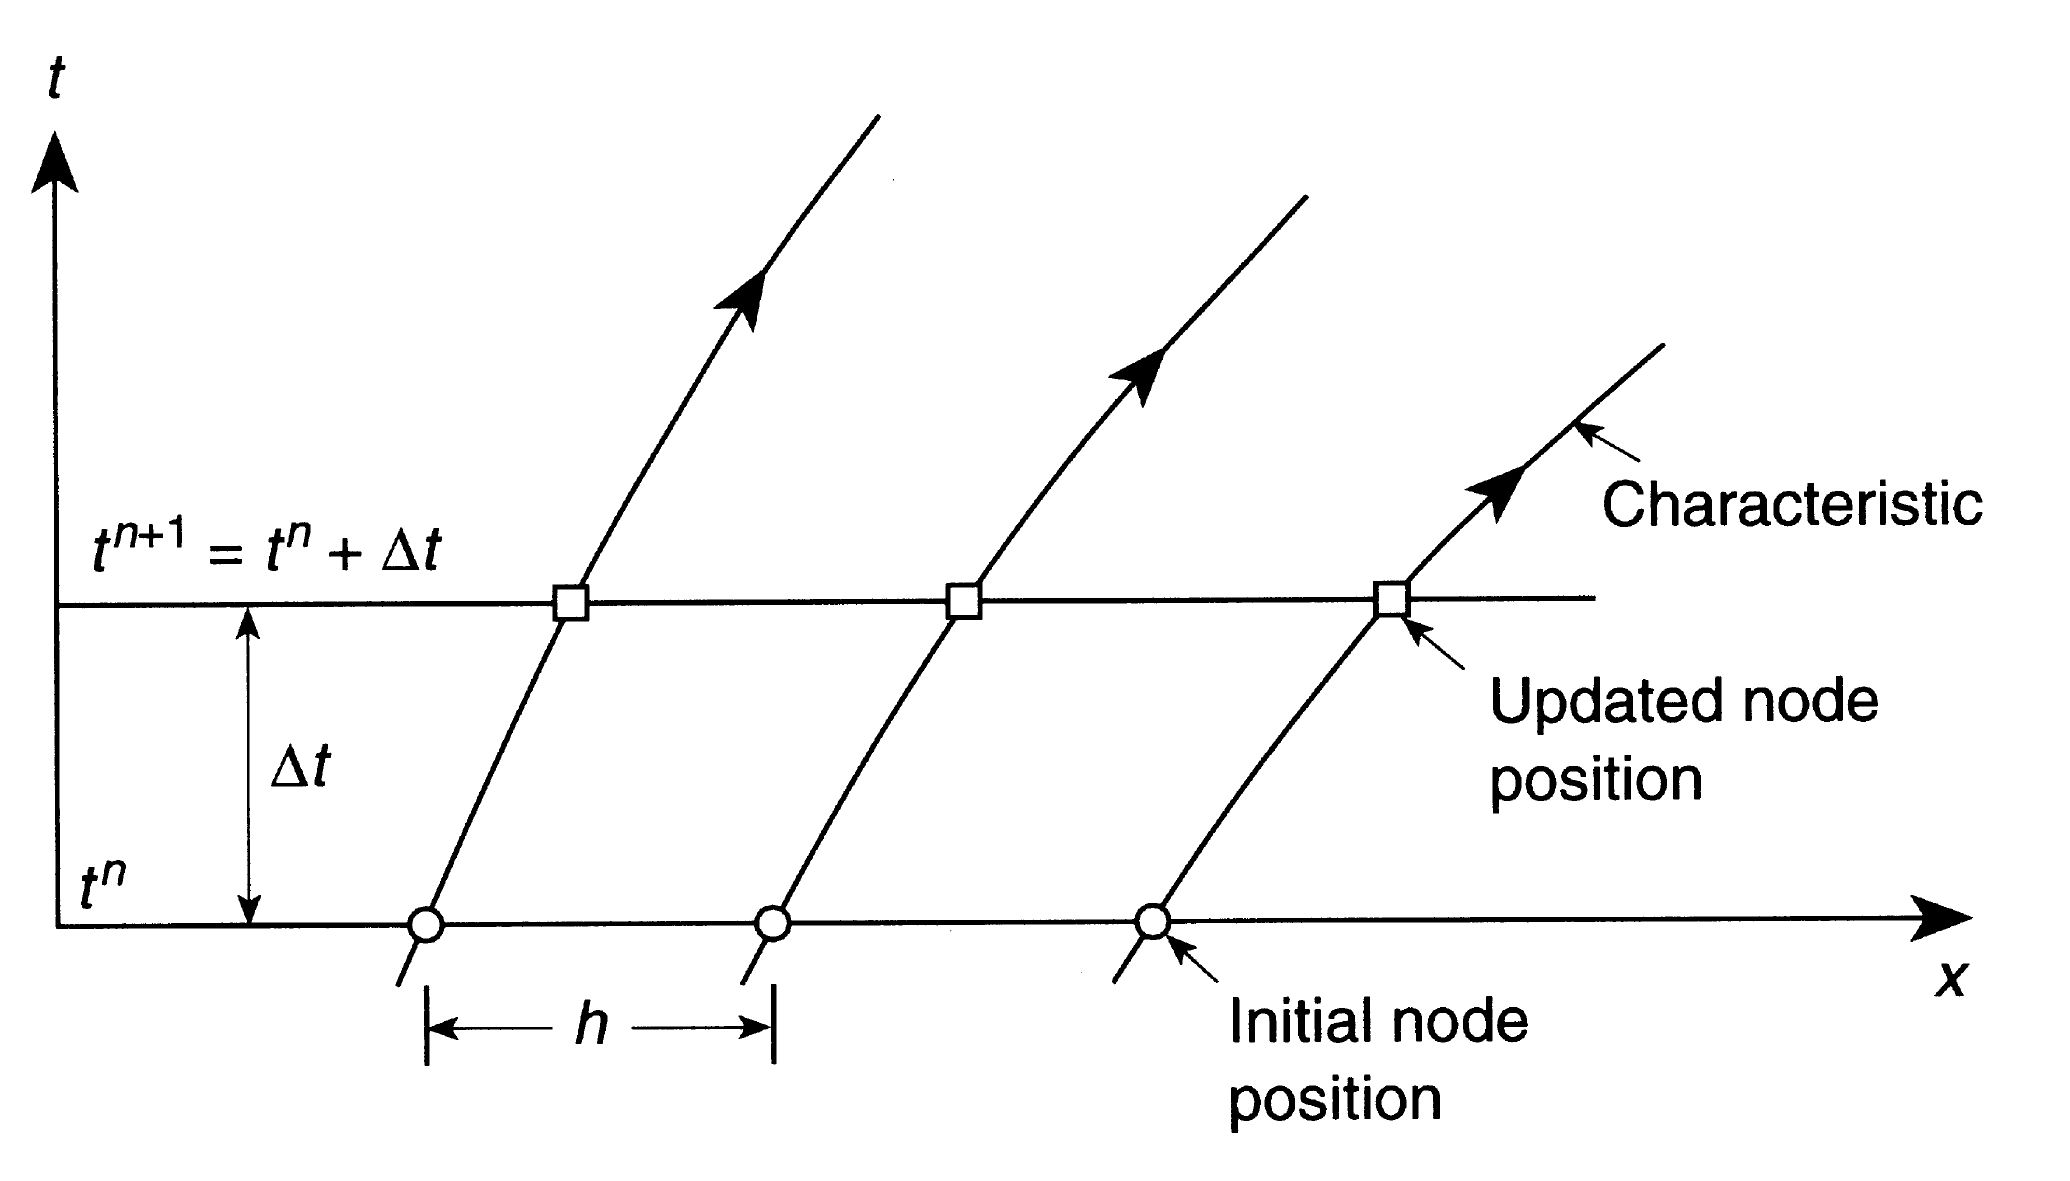
\includegraphics[scale=0.50]{Figures/fem_meshupdate_zienk_53.png}
\caption{Update of Mesh Nodes in FEM}
\label{fig:MeshUpdateFEM}
\end{figure}

\subsubsection{Problems with hyperbolic equations}

\section{Summary of Meshbased Methods}

One clear advantage of FDM and FVM over FEM is the simplicity of the Eulerian mesh.  Because the mesh stays fixed in space, independent from the fluids flow, these methods are also useful for highly deformations. But they come with a high computational costs, since in order to represent these deformations very fine meshes have to be used. This results also in much higher memory consumption that might lead to a limit what kind of fluid problem can be accurately simulated on given hardware. Furthermore FDM and FVM come with a inherently problem of domain communication. In contrast to FEM, both methods need to transport fluid matter from one mesh subdivision to the next during a flow process. This leads to a always necessary numerical communication between neighbouring subdivisions, no matter if a fluid is present in that cell or not. Consequently the domain decomposition on parallel systems leads to a more complicated communications between cluster machines.

%The fluids deformations, both methods do not involve the numerical problems of %Remeshing.

\begin{tabular}{|c|c|c|}
\hline
	Method & Discretization of & @\\
\hline
	FDM & differntial form of conservation equations & @\\
\hline
	FVM & integral form of conservation equations & @\\
\hline
\end{tabular}





% Chapter Template

\chapter{Smoothed Particle Hydrodynamics} % Main chapter title

\label{Chapter 5} % Change X to a consecutive number; for referencing this chapter elsewhere, use \ref{ChapterX}

\lhead{Chapter 5. \emph{Smoothed Particle Hydrodynamics}} % Change X to a consecutive number; this is for the header on each page - perhaps a shortened title

%----------------------------------------------------------------------------------------
%	SECTION 1
%----------------------------------------------------------------------------------------

\section{Mesh-free methods}
In this chapter the meshfree methods are introduced and explained on the example of the Smoothed Particle
Hydrodynamics method. For further reading \citep{Liu2003} is recommended.

\subsection{Why use mesh free methods?}

As described in Chapter 3 the scientific and engineering community have used mesh-based methods for
very long as they have cleary matured over the years. Still
Capability to work from
micro to macro scale applications.

The benefits of mesh-free methods versus classical mesh-based methods can be outlined as:
\begin{itemize}
\item Mesh-free methods can easily handle strong deformations that would lead to
remeshing in a FEM simulation. This is due to the absence of a topological mesh which in course
of a deformation simulation would lead to problems in connectivity. ShafonLi 15
\item The mesh-free discretization with particals can provide a better representation of a varying
geometric shape.
\end{itemize}

In this report we will focus on the Smoothed Particle Hydrodynamics method as one of the earliest
and vastly used mesh-free methods.

\subsection{History of SPH}

The idea of SPH was at first formulated in the year 1977.Its origins do not lie in CFD but in the attempt to model and solve astrophysical problems in a new way. Initially Gingold and Monoghan \citep{Gingold1977} invented and named this approach at the Institute of Astronomy in Cambridge. Their primary intention was to find a approach that would be less computational intensive than FDM to solve various evolution processes (e.g. a star forming from interstellar matter). In their article they state how limited the use of FDM
is for their often asymmetrical/distorted problems, since in order to be be computed accurately they needed a excessive amount of grid points (resp. high spatial discretization). They proposed a new way of discretization that was based on a Lagrangian description and used a fixed amount of randomly distributed particles. To model physical scalar and vector fields and to retrieve those values during computation they used statistical methods (Monte Carlo integral determination) along with a \emph{kernel function}. Their approach will be described in more detail in the following sections.  
Inspired by the colleagues at Cambridge, Lucy \citep{Lucy1977} used this numerical approach to test succesfully the feasability of the fission hypothesis for protostars, which is a gas dynamical problem of rotating fluids in space. In contrast to CFD, these problems like the formation of galaxies or solar systems are of macroscopic scale.
Today SPH and its further developments are widely adapted in astronomy, CFD and even VFX. 


\subsection{Applications of SPH}
Because of several numerical advantages of SPH it is today not only used in astrophysics but also in a wide
range of simulations for fluid dynamics like underwater explosions (e.g. Liu et al. ) and even fluid creation
for visual effects in feature film (see Chapter 4...) One of this visual effects applications will be explained
in more detail with the SPH software "Realflow" and NAIAD. For further reading on the applications of CFD in computer graphics please refer to \citep{Bridson2008} and for new Hybrid Methods that have the advantages of Meshbased and Meshfree methods \citep[pg. 195]{Jackl2006} provides a simple introduction. 


\begin{figure}[htp]
\centering
\begin{tabular}{cccc}
	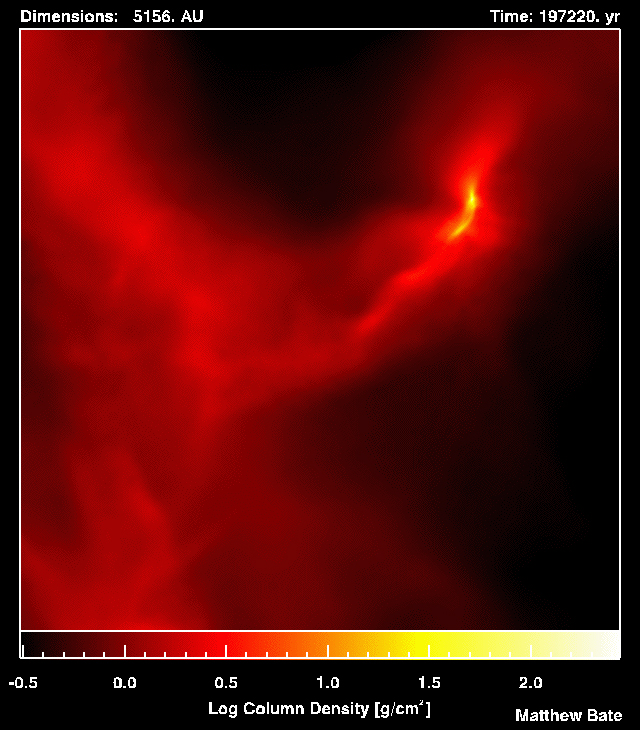
\includegraphics[width=0.2\textwidth]{Figures/sph_bates_starcluster_00.jpg} 
 &  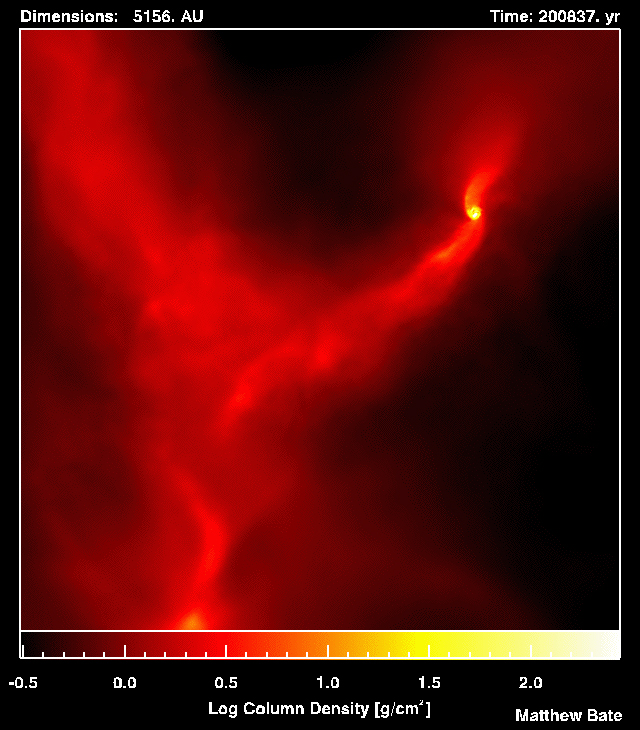
\includegraphics[width=0.2\textwidth]{Figures/sph_bates_starcluster_01.jpg} 
 &  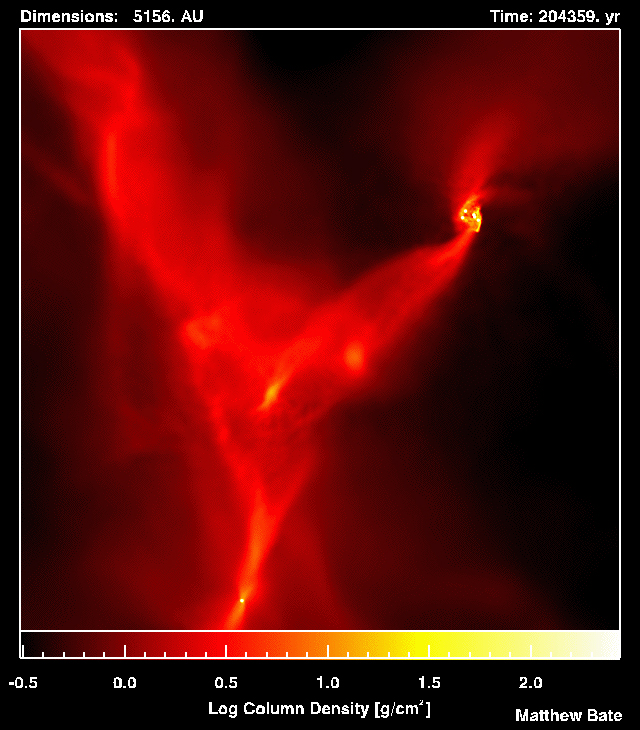
\includegraphics[width=0.2\textwidth]{Figures/sph_bates_starcluster_02.jpg}
 &  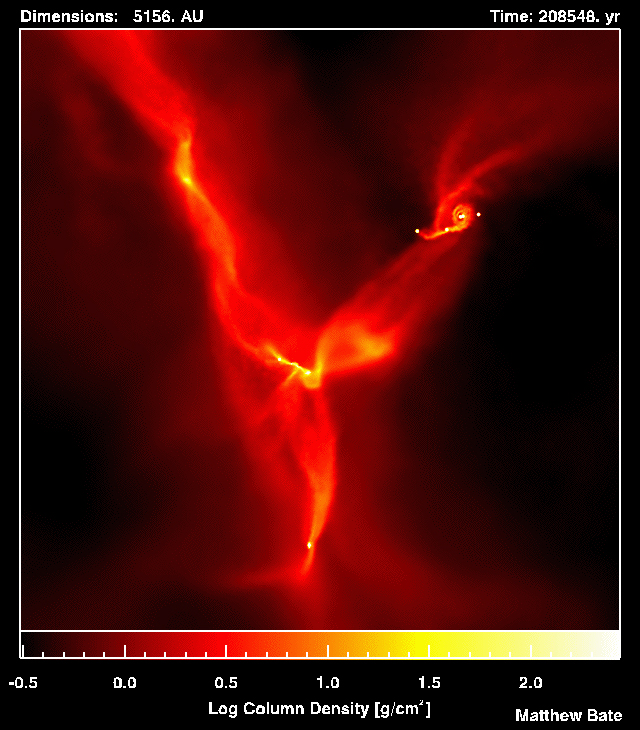
\includegraphics[width=0.2\textwidth]{Figures/sph_bates_starcluster_03.jpg}  
 \\
	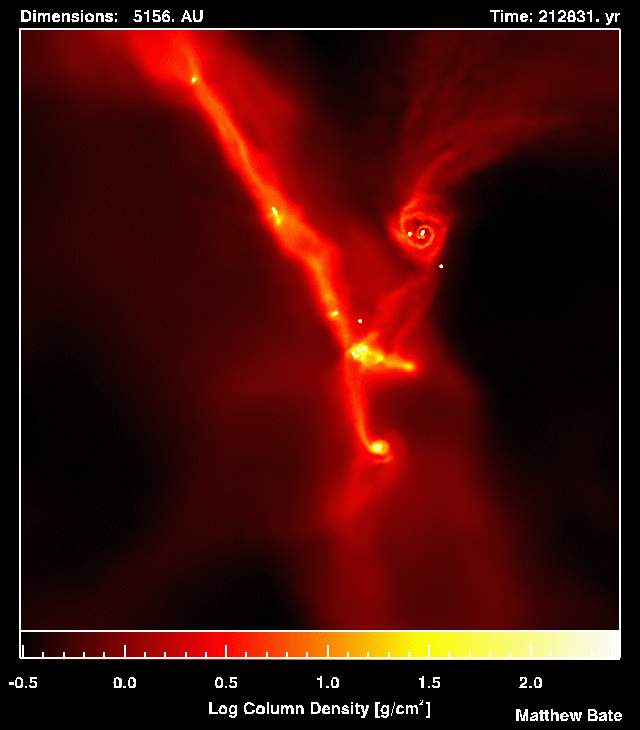
\includegraphics[width=0.2\textwidth]{Figures/sph_bates_starcluster_04.jpg} 
 &  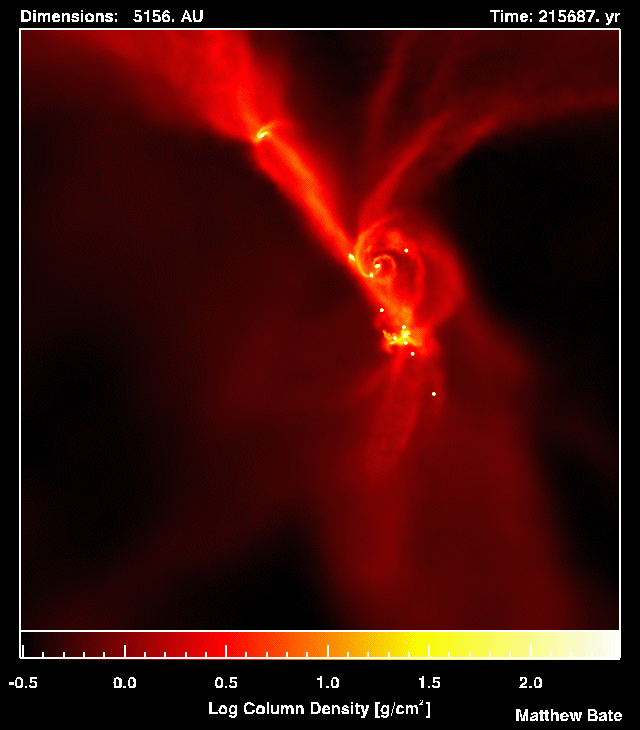
\includegraphics[width=0.2\textwidth]{Figures/sph_bates_starcluster_05.jpg} 
 &  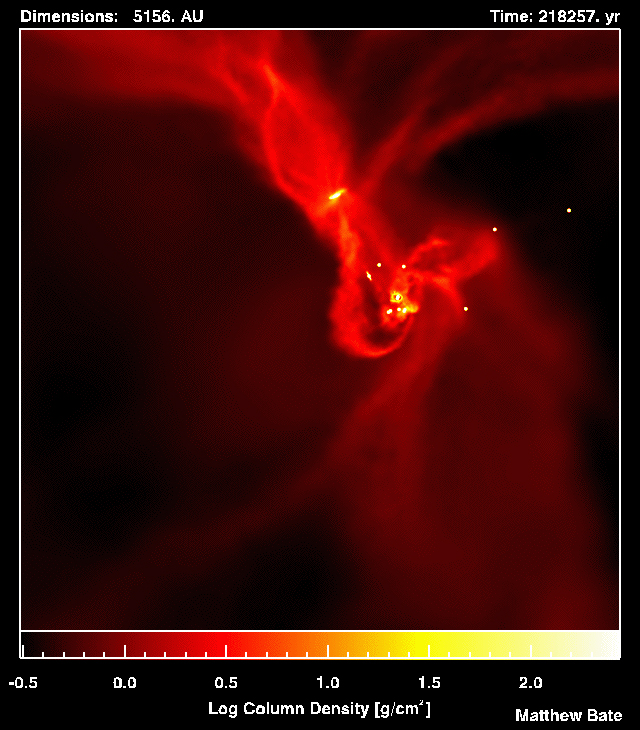
\includegraphics[width=0.2\textwidth]{Figures/sph_bates_starcluster_06.jpg}
 &  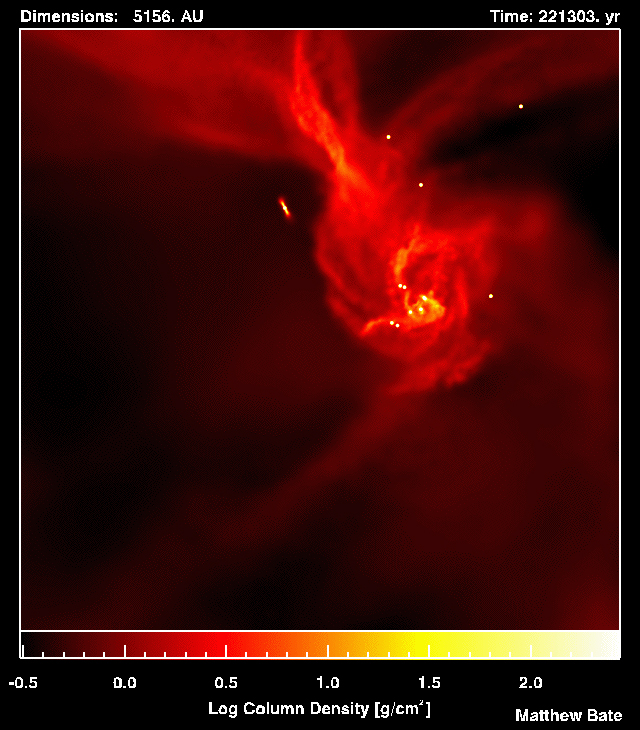
\includegraphics[width=0.2\textwidth]{Figures/sph_bates_starcluster_07.jpg} 
 \\
	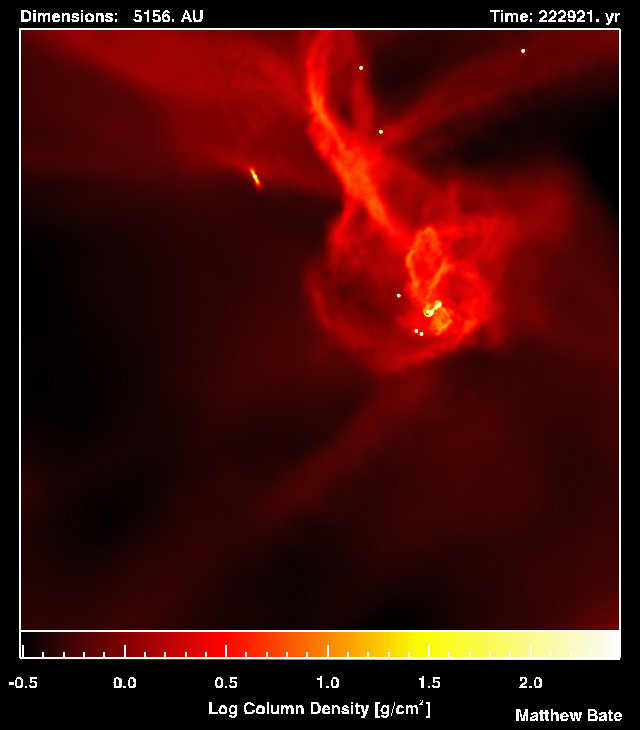
\includegraphics[width=0.2\textwidth]{Figures/sph_bates_starcluster_08.jpg} 
&   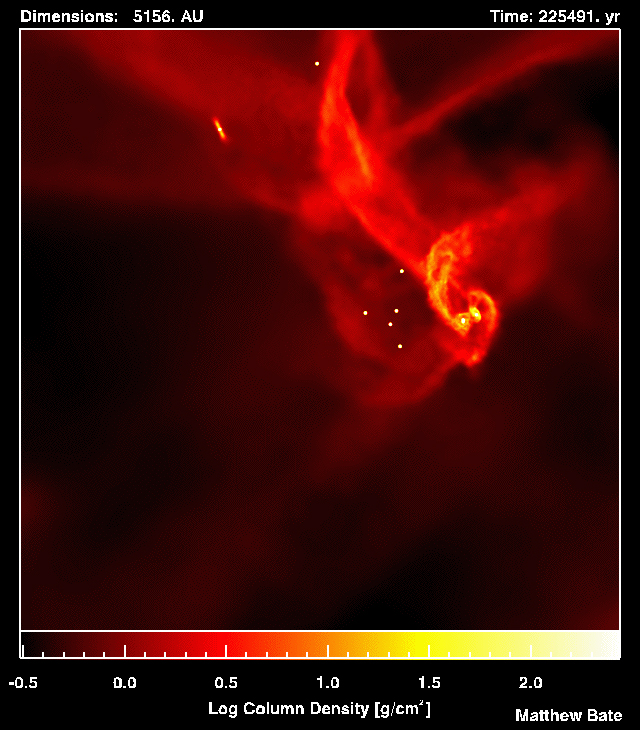
\includegraphics[width=0.2\textwidth]{Figures/sph_bates_starcluster_09.jpg}  
&   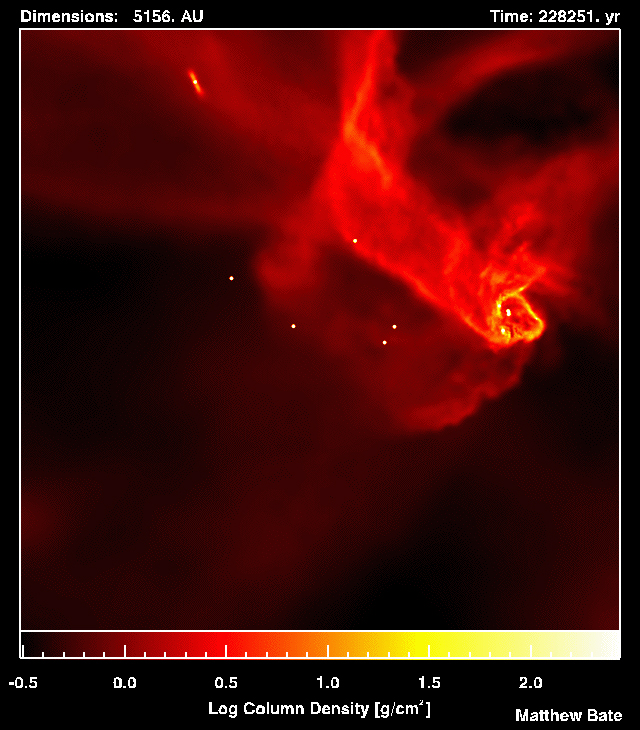
\includegraphics[width=0.2\textwidth]{Figures/sph_bates_starcluster_10.jpg}
&   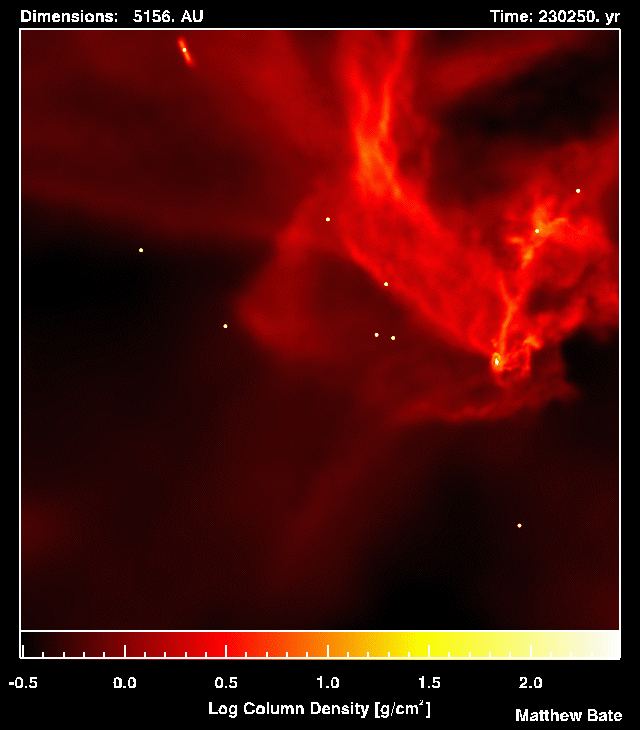
\includegraphics[width=0.2\textwidth]{Figures/sph_bates_starcluster_11.jpg} 
\\
	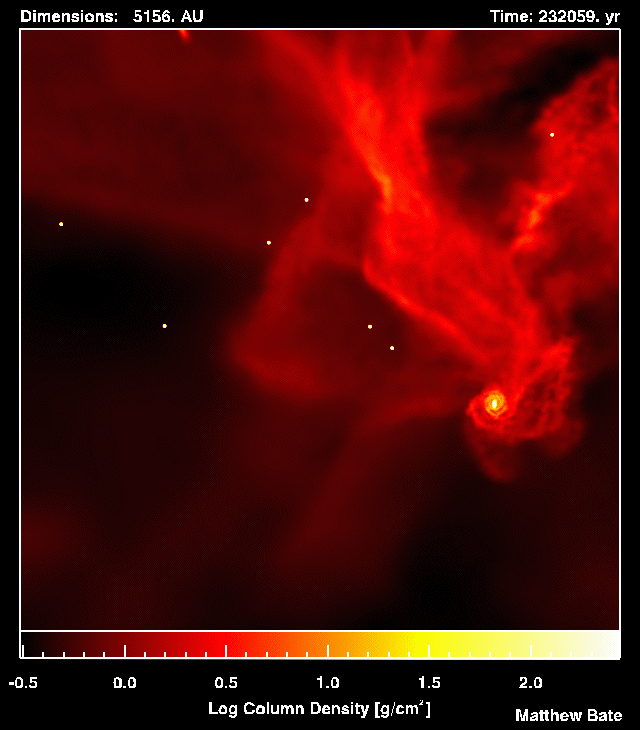
\includegraphics[width=0.2\textwidth]{Figures/sph_bates_starcluster_12.jpg} 
&   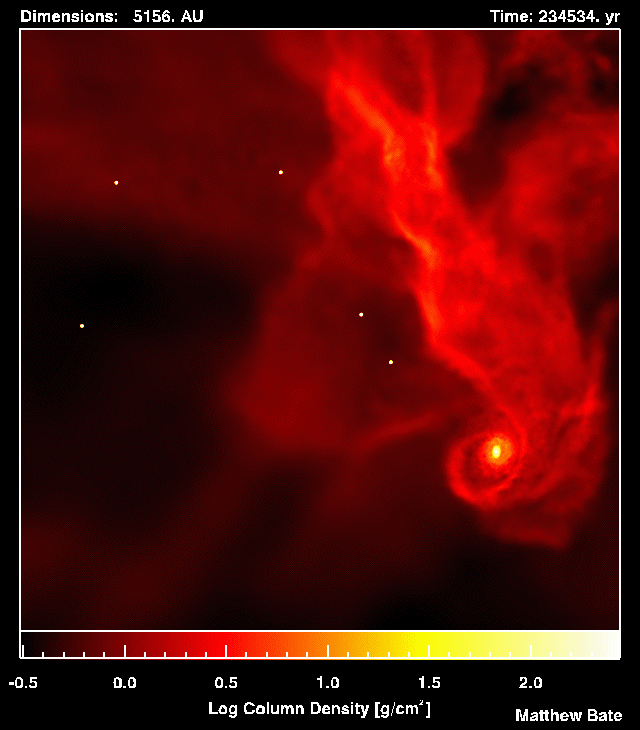
\includegraphics[width=0.2\textwidth]{Figures/sph_bates_starcluster_13.jpg}  
&   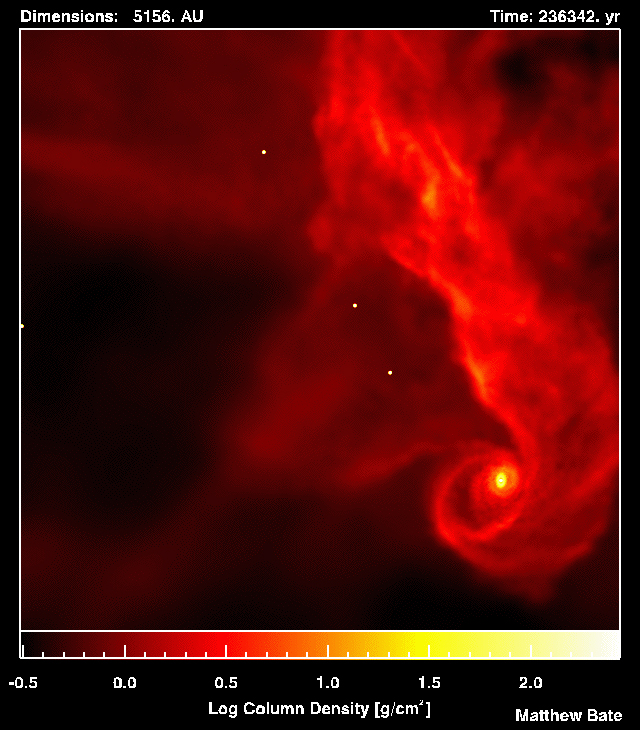
\includegraphics[width=0.2\textwidth]{Figures/sph_bates_starcluster_14.jpg}
&   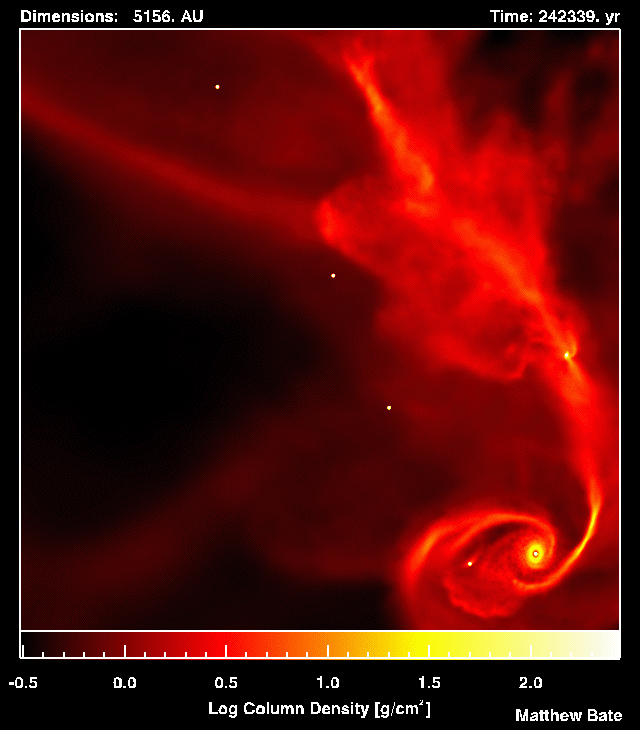
\includegraphics[width=0.2\textwidth]{Figures/sph_bates_starcluster_15.jpg}
\\

\end{tabular}
\caption{Image sequence of the Formation of Stars and Brown Dwarfs in a Star Cluster}
\label{fig:SPHStarCluster}
\end{figure}

\subsection{Basic idea of SPH}
SPH is a so called meshfree particle method (MPM) and replaces the meshbased discretization with a initial distribution of particles over the problem domain. 

\section{Mathematical foundation}

In order to discretize a domain with particles, the mathematical foundations differ greatly from Meshbased methods. Similar to FVM a integral representation of fluid variables is needed. For a continuous function $f(x)$ that has the mathematical preconditions to be represented in a integral form, it can be written in integral form as follows:

\begin{equation} \label{eq:func_intg_dirac}
f(x) = \int_{\Omega} \biggl [ f(a) \delta(x-a) \biggr ] d a \ \ \ (x, a) \in \Omega
\end{equation}

With the Dirac delta function being:

\begin{equation}
\label{eq:dirac_delta_fu}
\delta(x-a)= 
\begin{cases} 
1, & \mbox{if } x = a \\ 
0, & \mbox{if } x \neq a
\end{cases}
\end{equation}


Where $ \Omega $ represents the problem domain with the vectors $ x  a $ in it. Because of the Dirac delta function \ref{eq:dirac_delta_fu} the integral formulation becomes zero at all vectors except the exact vector x. The form \ref{eq:func_intg_dirac} is of great importance to SPH methods. It allows the Dirac delta function $\delta$ (which produces a exact equality)  to be replaced by a \emph{kernel function} K which leads to the approximation:

\begin{equation} \label{eq:func_intg_kernel}
f(x) \approx \int_{\Omega} \biggl [ f(a) K(x-a) \biggr ] d a \ \ \ (x, a) \in \Omega
\end{equation}

In the equations of fluid dynamics, often the divergence operator is found. The divergence of a vector function $\nabla \cdot f(x)$ can be similarly
written like the above notation:

\begin{equation} \label{eq:func_intg_kernel_div}
\nabla \cdot f(x) \approx \int_{\Omega} \biggl [ \nabla \cdot f(a) K(x-a) \biggr ] d a \ \ \ (x, a) \in \Omega
\end{equation}
 

In the following section this kernel function is further discussed in brought into a form where it can be discretized.

\subsection{Kernel approximation}
The kernel function K can be rewritten with another parameter $h$, which as we will see is used for a similar limit formulation, as it is found in the equations of Meshbased methods. Furthermore due to a already established conventions in SPH, the bracket operator $ < >$ is used to 
clearly visualize that function $f(x)$ is approximated by the kernel function K:

\begin{equation} \label{eq:func_intg_kernel_h_brk}
< f(x) > = \int_{\Omega} \biggl [ f(a) K(x-a, h) \biggr ] d a \ \ \ (x, a) \in \Omega
\end{equation}

The bracket operator can be also used to rewrite equation \ref{eq:func_intg_kernel_div}:

\begin{equation} \label{eq:func_intg_kernel_h_brk_div}
< \nabla \cdot f(x) > = \int_{\Omega} \biggl [ \nabla \cdot f(a) K(x-a, h) \biggr ] d a \ \ \ (x, a) \in \Omega
\end{equation}

The relation between the Dirac delta function and the kernel function K can be written down with the limit notation by:

\begin{equation} \label{eq:kernel_vs_dirac}
\lim_{h \to 0} K(x-a, h) = \delta(x-a)
\end{equation}

Similar to equation \ref{eq:fdm_con} in FDM, the value of $ h $ is used to approximate a function. In contrast to FDM though, not the function itself that should be discretized is approximated, but the Dirac function. Equation \ref{eq:kernel_vs_dirac} represent the \emph{Delta function condition}, which is one out of three conditions that has to be met my the kernel function K, in order to be used with SPH. For further reading on the \emph{unity condition} and the \emph{compact condition} please refer to \citep[pg. 37]{Liu2003}. From now on we will call $ h $ the kernel \emph{length}. In literature the term \emph{kernel} is often used in exchange with the term \emph{smoothing}, which result in smoothing function K and smoothing length $h$. In this report the term kernel will be used. The problem domain $ \Omega $ is also called \emph{support domain}.\footnote{This is a simplification for this report. Strictly speaking the support domain can also be outside of the problem domain and therefore not equivalent.}  

The equation \ref{eq:func_intg_kernel_h_brk_div} can be rewritten to: 

\begin{equation} \label{eq:func_intg_kernel_h_brk_div}
< \nabla \cdot f(x) > = 
\overbrace{\int_{\Omega} \nabla \cdot \biggl [ f(a) K(x-a, h) \biggr ] d a}^{Divergence\ theorem\ applicable} -
\int_{\Omega} \biggl [ f(a) \cdot \nabla K(x-a, h) \biggr ] d a
\end{equation}

This form allows to apply the \nameref{sec:div_theorem} , onto the RHS of the equation:

\begin{equation} \label{eq:func_intg_kernel_h_brk_div_theo}
< \nabla \cdot f(x) > = 
\int_{A} \biggl [ f(a) K(x-a, h) \cdot \vec{n}  \biggr ] d A -
\int_{\Omega} \biggl [ f(a) \cdot \nabla K(x-a, h) \biggr ] d a
\end{equation}

For vectors a which are not identical to vector x, and for which the distance between them bypasses the kernel length  $|(x-a)| > h $  the kernel function becomes zero. This leads the integral of the surface A which is located inside the problem domain $\Omega$ to be zero. Therefore the equation simplifies to:

\begin{equation} \label{eq:func_intg_kernel_simple}
< \nabla \cdot f(x) > = 
- \int_{\Omega} \biggl [ f(a) \cdot \nabla K(x-a, h) \biggr ] d a
\end{equation}

Considering the conversion of equation \ref{eq:func_intg_kernel_div} to \ref{eq:func_intg_kernel_simple} with the help of the divergence theorem, something remarkable has happened. The divergence operation on the vector function $f(x)$ has been shifted to be a gradient operation at the kernel function K, leaving the vector function untouched. Therefore the kernel approximation in SPH which was used to represent the field function f in a integral form has the following advantage: When a divergence operation occurs at the field function (which often happens in CFD), the solution can be computed by the values of the function itself and the gradient of the kernel function, without caring about the divergence of the function. This will lead to much simpler and faster solvable equations. Now that the continuous integral forms are written in the kernel approximation form, in the next step the equations \ref{eq:func_intg_kernel_h_brk} and \ref{eq:func_intg_kernel_simple} can be finally discretized using particles.

\subsection{Particle approximation}

In order to discretize the continuous integral form that are represented by the kernel approximations, the SPH method uses particle summations. In the beginning of the process the domain is discretized or better split up into randomly distributed system of particles. These particles carry certain values like mass and density. The problem of correctly distributing the particles is further discussed in the Implementation sections of this report. 
In discretized form the particles represent the overall domain $\Omega$. To compute the physical values at a certain point (or particle) inside the domain, the surrounding particles are considered and a weighted average value is computed. This entire process will be discussed in this Section.

For simplicity and better understanding we first assume a already discretized domain with randomly distributed particles. Figure \ref{fig:sph_par_approx_domain} illustrates the two dimensional distribution of these particles in the domain $\Omega$. The region from which field information should be computed is marked as the red particle $i$. This particle is surrounded by a \emph{support domain} (dotted quadratic line) that defines which particles have influence on the field variable values it inhibits. This support domain is controlled by the kernel function K and its kernel length $h$. In the illustration the support domain is simplified as a two dimensional area, but it can also be a spheric volume with radius $h$ or of any other shape that depends on the kernel length. The magnitude of influence is illustrated by
a bell shaped kernel function, that clearly decreases with increasing distance from the particle $i$. Now to transform the idea of this illustration into the mathematical particle approximation of SPH, we consider the support domain to be a cubic volume $V$  with side length $h$.


\begin{figure}[htb]
\centering
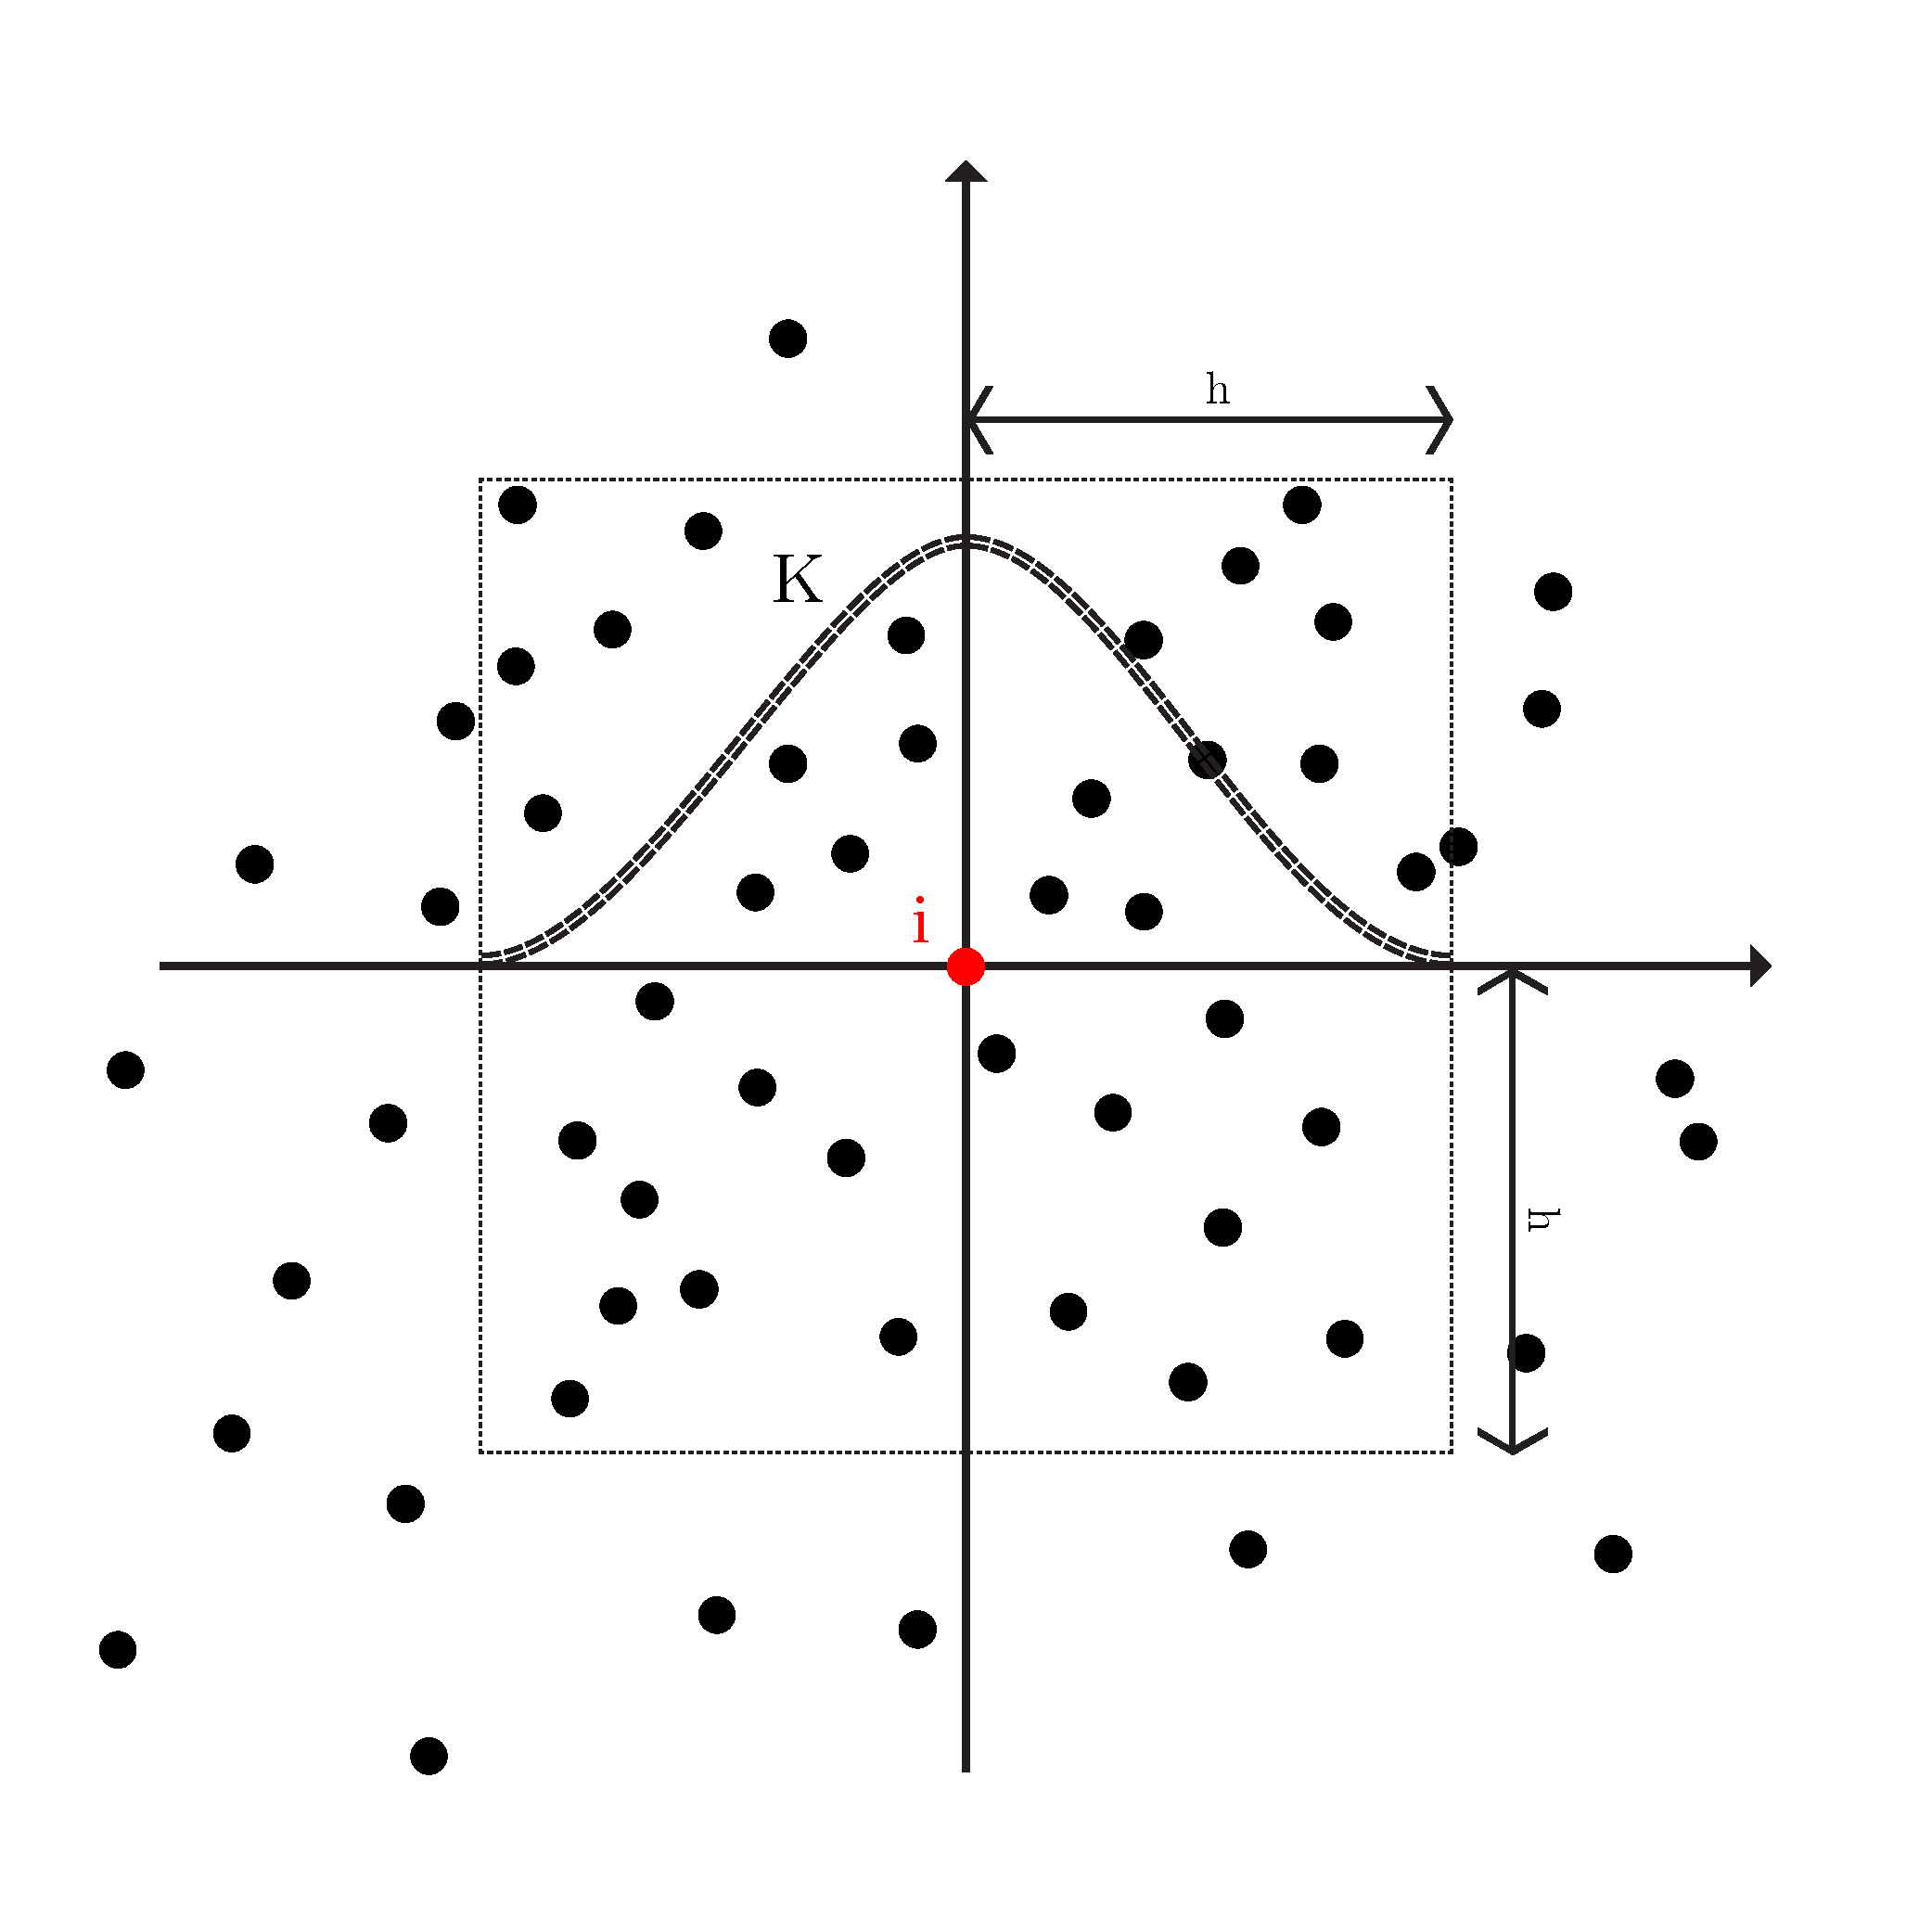
\includegraphics[width=0.8\textwidth]{Figures/sph_particle_domain.pdf}
\caption{Illustration of particle approximation with kernel function K and quadratic support domain}
\label{fig:sph_par_approx_domain}
\end{figure}

The domain $\Omega$ is discretized into a finite amount of $N$ particles. Each particle $j$ is assigned a mass $m_{j}$ and a density $\rho_{j}$, which are equal fractions of the total mass and density of $\Omega$. The mass of particles $m_{j}$ inside the cubic support volume $V_{j}$ can therefore be written as:

\begin{equation} \label{eq:sph_volume_mass}
m_{j} = V_{j}\rho_{j} \ \ \ j \in V_{j}
\end{equation}

Considering the kernel approximation equation \ref{eq:func_intg_kernel_h_brk}, the integral over the continuous domain $\Omega$ can now be rewritten to a discrete summation:

\begin{equation} 
\label{eq:kernel_to_part_approx}
\begin{split}
< f(x_{i}) > 
&= \int_{\Omega} \biggl [ f(a) K(x-a, h) \biggr ] d a \\
&\approx    \sum_{j=1}^{N} \biggl [ f(a_{j}) K(x_{i}-a_{j}, h) V_{j} \biggr ]
\end{split}
\end{equation}

In equation \ref{eq:kernel_to_part_approx} the step from kernel approximation to particle approximation has been made. Now the vectors $x_{i}$, $a_{j}$ represent particle positions. Thereby the function is approximated at particle $i$. This equation can be further written with a rearranged equation \ref{eq:sph_volume_mass} in mind to:

\begin{equation} 
\label{eq:kernel_to_part_approx_mass_dens}
\begin{split}
< f(x_{i}) > 
&\approx    \sum_{j=1}^{N} \biggl [ f(a_{j}) K(x_{i}-a_{j}, h) V_{j} \biggr ] \\
&=          \sum_{j=1}^{N} \biggl [ f(a_{j}) K(x_{i}-a_{j}, h) \frac{m_{j}}{\rho_{j}} \biggr ] \\
&=          \sum_{j=1}^{N} \biggl [ \frac{m_{j}}{\rho_{j}}  f(a_{j}) K(x_{i}-a_{j}, h) \biggr ] 
\end{split}
\end{equation}

Note that in equation \ref{eq:kernel_to_part_approx_mass_dens} the only changing input values are the particle properties (e.g. position, mass, density, ...) of the  the particle(s) $i,j$. Furthermore the most significantly varying element in the equation is the kernel function K itself. Most SPH methods can be clearly identified by the kernel function they use to weight the influence of surrounding particles. Therefore the equation can become cleaner by separating the kernel function $K_{i,j}$ 
from the description:

\begin{equation} 
\label{eq:kernel_to_part_clean}
< f(x_{i}) > =
\sum_{j=1}^{N} \frac{m_{j}}{\rho_{j}}  f(a_{j}) \cdot K_{i,j}
\end{equation}

Similar to the kernel approximation in equation \ref{eq:func_intg_kernel_h_brk} the particle approximation can be applied to \ref{eq:func_intg_kernel_simple}, which finally leads to:

\begin{equation} \label{eq:kernel2_to_part_clean}
< \nabla \cdot f(x) > = 
- \sum_{j=1}^{N} \frac{m_{j}}{\rho_{j}}  f(a_{j}) \cdot \nabla K_{i,j}
\end{equation}

In this Section the kernel approximations were discretized to the particle approximations. These two approximations and the step to latter are the mathematical cornerstone of the SPH method. The continuous integrals from the kernel approximations were transformed to summations over a finite amount of particles inside a finite support domain. This particle approximation is done at each time step of the simulation. Note that this simple idea of a averaged summations with particles was done completely without the presence of a mesh. Each particle was associated with at least properties for position, mass and density. As we will see in later Sections, further physical properties can be associated with particles for hydrodynamic problems. How the distribution of particles is done, will be discussed in later Sections. In the following Sections these mathematical framework is used to implement the NSE with SPH. Hereby to consider are algorithms to efficiently determine, which particles are inside the support domain.



\subsection{Lagrangian Navier-Stokes equations}
Because SPH is a pure Lagrangian method, also the NSE need to be formulated in the Lagrangian form. In the previous Chapters mostly the Eulerian forms were used. 

\subsection{SPH vs. FEM}
While both methods in most implementations share a Lagrangian perspective the main difference between the
FEM and particle based methods is indeed the absence of a overall grid in the SPH methods. While FEM is based
on finite elements, they still exist within a grid.

For further reading please refer to \citep{Li2004} and \citep{Liu2003}.

\subsection{Benefits of Meshfree methods over Meshbased methods}
The most problems of the Meshbased methods result not from the numerical capabilities of their methods, but from the simple presence of a mesh itself. 

item Be@tter to model physcal behaviour that has strong distortion
item Mesh dependend problems like re³meshing are avo§ided
item No tie-consuming (re-)genera§tion of meshes for a problem 

%-----------------------------------
%	SUBSECTION 2
%-----------------------------------
\section{Implementation}

\subsection{Nearest neighbour particles}

\subsection{Issues of computer implementation}
%RAM...

\subsection{Parcallel Coding}


Fitc


\section{Implementation of Navier-Stokes equations}


\section{Particle consistency problem}

% Chapter Template

\chapter{Useage in Simulation Software} % Main chapter title

\label{Chapter 6} % Change X to a consecutive number; for referencing this chapter elsewhere, use \ref{ChapterX}

\lhead{Chapter 6. \emph{Useage in Simulation Software}} % Change X to a consecutive number; this is for the header on each page - perhaps a shortened title

%----------------------------------------------------------------------------------------
%	SECTION 1
%----------------------------------------------------------------------------------------

\section{Mesh-free methods}


\subsection{Why use mesh free methods?}



%-----------------------------------
%	SUBSECTION 2
%-----------------------------------
\section{Implementation}

 

%\input{./Chapters/Chapter7} 

%----------------------------------------------------------------------------------------
%	THESIS CONTENT - APPENDICES
%----------------------------------------------------------------------------------------

\addtocontents{toc}{\vspace{2em}} % Add a gap in the Contents, for aesthetics

\appendix % Cue to tell LaTeX that the following 'chapters' are Appendices

% Include the appendices of the thesis as separate files from the Appendices folder
% Uncomment the lines as you write the Appendices
%\cite{Reference3}
%% Appendix A

\chapter{Appendix Title Here} % Main appendix title

\label{AppendixA} % For referencing this appendix elsewhere, use \ref{AppendixA}

\lhead{Appendix A. \emph{Appendix Title Here}} % This is for the header on each page - perhaps a shortened title

Write your Appendix content here.
%\input{./Appendices/AppendixB}
%\input{./Appendices/AppendixC}

\addtocontents{toc}{\vspace{2em}} % Add a gap in the Contents, for aesthetics

\backmatter

%----------------------------------------------------------------------------------------
%	BIBLIOGRAPHY
%----------------------------------------------------------------------------------------

\label{Bibliography}

\lhead{\emph{Bibliography}} % Change the page header to say "Bibliography"

\bibliographystyle{plainnat} % Use the "unsrtnat" BibTeX style for formatting the Bibliography

\bibliography{Bibliography} % The references (bibliography) information are stored in the file named "Bibliography.bib"

\end{document}  
